%%==================================================
%% thesis.tex
%%==================================================

% 双面打印
\documentclass[master, macfonts, openany, cs4size]{TJUgraduates} 
% \documentclass[bachelor, adobefonts, openright, cs4size]{TJUgraduates} 
% \documentclass[master]{TJUgraduates} 
% \documentclass[%
%   bachelor|master|doctor 
%   adobefonts, winfonts  	% 修改 /ctex 中的adobefonts, 改为mac默认中文字体
%   openany|openright 		% 单面打印,双面打印(默认)
%   cs4size|c5size 		% 正文字号:小四、五号(默认)
% ]

\usepackage{siunitx}
\usepackage{booktabs}
\usepackage{textcomp}
\usepackage{paralist}

\begin{document}
\title{软管组件纤维编织增强层
	\vskip 5pt
非线性本构关系研究及试验测试}
\projectsource{企事业单位委托项目 ~~ 编号:20131934}

\author{胡牧原}
\advisor{贺鹏飞 ~ 教授}
\viceadvisor{郑百林 ~ 教授}
\defenddate{二〇一五年三月}
\school{同济大学}
\institute{力学系}
\studentnumber{1233907}
\major{力学}
\discipline{工学}
\faculty{航空航天与力学学院}

\englishtitle{A Study  on Nonlinear Constitutive Relation  of 
	Braided Fiber Reinforcement Layers in  Hose \vskip 5pt Assembly and Experiment}
\englishauthor{\textsc{Hu Muyuan}}
\englishadvisor{Prof. \textsc{ He Pengfei}}
\englishviceadvisor{Prof. \textsc{ Zheng Bailin}}
\englishschool{Tongji University}
\englishinstitute{\textsc{Depart of XXX, School of XXX} \\
  \textsc{ Tongji University} \\
  \textsc{Shanghai, P.R.China}}

\englishdiscipline{Engineering}
\englishfaculty{School of Aerospace \\
Engineering and Applied Mechanics}

\englishmajor{Mechanics}
\englishdate{March, 2015}




%% 无编号内容:中英文论文封面、授权页

\maketitle

\makeenglishtitle

\makeDeclareAuthorization
\makeDeclareOriginal


\frontmatter 	% 使用罗马数字对前言编号

%%==================================================
%% abstract.tex for SJTU Master Thesis
%% based on CASthesis
%% modified by wei.jianwen@gmail.com
%% version: 0.3a
%% Encoding: UTF-8
%% last update: Dec 5th, 2010
%%==================================================

\begin{abstract}
随着我国航空航天事业的蓬勃发展,软管组件作为液压系统中的重要元件,其设计生产水平的要求也迅速提高。软管组件一般采用金属纤维编织的形式,而最新一代非金属纤维编织加强的软管也已在国外先进机型广泛使用。本研究针对这种纤维编织的加强层开展了研究,深入分析了这类结构的整体力学性能,以及纤维间的细观力学行为对编织加强层性能的影响。

研究思路主要基于Hachami  2011年提出的金属编织层本构理论,因为该理论能够有效的结合加强层理论体系中的基于“钢绞线理论”的方法以及基于复合材料的方法。

研究过程中,以及拉伸实验的研究方法,对不同尺寸金属编织软管进行了拉伸实验。发现金属纤维编织层在拉伸时会出现强烈的结构非线性,而该理论不能在非线性段与实验结果相吻合。针对这种情况,提出了一系列修正该理论的方法:

1.将金属纤维间交叠产生的接触等效地转化为“修正基体”(Modified Matrix Method),独立于金属纤维自身产生的刚度,对特征单元的刚度矩阵进行了补充,使其能够满足三维有限元计算的需要。

2.对Hachami 模型编织角理论部分进行了修正,还提出了编织角加速系数$ k $的概念,并对其物理意义进行了讨论。

3.Hachami 模型中“特征单元”并没有考虑编织层中纤维的上下起伏,导致模型偏刚,影响到内压荷载的计算结果。考虑纤维的空间取向,利用弯曲纤维模型的简化方法对特征单元的刚度矩阵进行了修正。

本研究的创新点主要有:
1.新的研究对象。尽管软管组件的纤维编织加强层已出现超过半个世纪,其指导设计的理论仍然是简单“薄壁圆柱”的受力平衡,经验公式以及实验;区别普通的纤维加强符合材料,编织加强层没有树脂相,是一种柔性的、表现出结构非线性力学行为的结构。

2.编织加强层非线性段的力学行为分析。由于这种结构的复杂性,以往无论基于解析还是数值的分析方法,较少有进入到编织层发生大变形,产生较大非线性的力学行为阶段的。

3.修正刚度的方法。许多复合材料力学常见的修正方法第一次被引进编织加强层的理论体系中。而以往的编织层理论都是过度简化,不能考虑纤维间复杂相互关系的。

4.仿真内压爆破的方法。内压爆破试验是设计编制加强层 的核心试验,仿真内压荷载需要主要是为了确定内压荷载与加强层纤维应力的关系,也需要一套可行的强度理论。基于准静态的仿真,结合材料力学中突加荷载理论,提出了一套可以准确仿真内压爆破试验的方法。

  \keywords{\zihao{-4} 
  	编织 \quad 
  	软管 \quad 
  	接头\quad 
  	拉伸实验\quad 
  	修正基体\quad 
  	复合材料\quad 
  	纤维\quad 
  	仿真\quad 
  	爆破试验\quad 
  	}
\end{abstract}

\begin{englishabstract}

Flexible hose assembly has always been one of the most vital parts within the hydraulic system of the aircrafts, which are used in industry for power transmission in steering, drive and brake systems and for fluid transport. Such hoses must be tight, flexible, and resistant against high inside pressure. Reinforcement layers bear the most pressure load, commonly formed with braided or helical-wounded metal wires and composite fibers.

The purpose of this work is to develop a realistic numerical simulation model for different types of high-pressure hydraulic hoses. The goals of this research are realistic prediction of the deformation and stress response under service loads, determination of the bursting pressure. The model proposed by Hachemi in 2011 is chosen as the base theory for the work, since it is regarded as an mixture of two major branches of the current hose theory, and focusing on the macro mechanical behavior of braid reinforcement layers in the form of tubes.

It has been discern during the research that Hachemi's theory is not keeping up with our experimental results which shows far more non-linearity than the theory predict.
Several modifications and developments to the theory has been put forward, in order to match the non-linearity, by accounting for the interactions between the metal wire of composite fibers.




\textbf{main jobs:}
\begin{compactenum}
	\item  introduced a “modifying matrix”, from composites mechanics, to detach inter-wire contacts from wire elongation. 
	
	\item  modified the representative unit cell  and  also proposed a hypothesis opposite to Hachemi’s one: the braid angle decreased linearly, applied displacement load with constant loading rate, rather than locked at a certain degree. 
	\item  we introduce a modification coefficient , accelerating the decrease of braid angle to match the nonlinearity in force-displacement curve. Lateral contact is considered to be the factor of excessively decreased braid angle when the calculated curve perfectly meet the experimental one.

\end{compactenum}

\textbf{Innovations:}
\begin{compactenum}
	\item Introduce a relatively new subject. Although these hoses have been in production for over a hundred years, most information concerning their usage, ratings, and design have been empirical in nature or based solely on equilibrium considerations of inextensible reinforcement.
	\item Few research has been done in the field of nonlinear behavior of the braid reinforcement. Methods commonly used in composite mechanics are introduced for the first time to take  forms of nonlinear material behavior into account.
	\item A numerical simulation of hose under burst pressure load has been done,  helping to determined the failure criteria of fiber or metal wire.



\end{compactenum}



  \englishkeywords{\zihao{-4}  
  	hose assembly, 
  	PTFE, 
  	fiber,
  	reinforcement}
  
  
\end{englishabstract}
 %% 摘要
%% 目录、插图目录、表格目录
\tableofcontents

\listoffigures
\addcontentsline{toc}{chapter}{\listfigurename} %将插图目录加入全文目录

\listoftables
\addcontentsline{toc}{chapter}{\listtablename}  %将表格目录加入全文目录

%%==================================================
%% symbol.tex for SJTU Master Thesis
%% based on CASthesis
%% modified by wei.jianwen@gmail.com
%% version: 0.3a
%% Encoding: UTF-8
%% last update: Dec 5th, 2010
%%==================================================

\chapter{主要符号对照表}
\label{chap:symb}


\begin{center}
	

\vspace{1cm}
\begin{tabular}{ll}

$\epsilon$       & \hspace{5em}介电常数 \\
$\mu$ \qquad     & \hspace{5em}磁导率 \\


\end{tabular}


\end{center}
 % 主要符号、缩略词对照表


\mainmatter	% 使用阿拉伯数字对正文编号

%% 正文内容
%%==========================
%% chapter01.tex for TJU Master Thesis
%% based on CASthesis
%% modified by charlie.yaha@gmail.com
%% version: 0.1alpha
%% Encoding: UTF-8
%% last update: Dec 5th, 2010
%%==================================================

%\bibliographystyle{TJU} %[此处用于每章都生产参考文献]


\chapter{绪~论}
\label{chap:introduintroduction}
%了解什么事软管
\section{研究背景}
%软管定义,软管组件结构
编织加强软管由内管、纤维增强层及金属连接件组成,是一种复合结构的管路连接件,一般将整个系统结构称为软管组件(Flexible Hose Assembly),或软管总成(本文统一称为软管组件)。
其结构如图\ref{fig:hose structure}所示:柔性内管,例如橡胶管,氟塑料管,金属波纹管,其外外包覆若干层柔性加强结构(编织、缠绕),主要承受内管的内压荷载,加强层数一般视内压荷载大小而定。软管组件工作时,绝大部分内压荷载由编织层承担,内管主要起通道的作用。


\begin{figure}[!htbp]
\centering
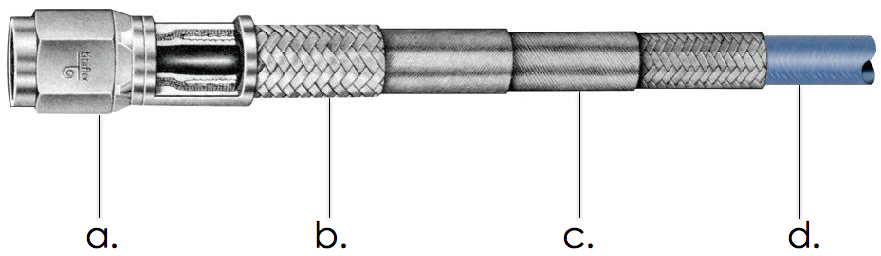
\includegraphics[width=0.6\linewidth]{figure/chap1/Hose-Structure}
\bicaption[fig:hose structure]{软管组件结构}{软管组件结构(a.接头,b.金属纤维编织层,c.金属纤维缠绕层,d.内管)}{Fig}{Hose Structure(a.Coupling,b.Braid Layer,c.Helix-wound Layer,d.Inner Tube)}
\label{fig:hose structure}
\end{figure}


软管组件主要应用于液压、气动、燃油、滑油等系统的介质传输,起到了“血管”作用,航空航天飞行器、汽车、船舶,以及各种工业设备、机床等,都大量使用了软管组件。如图\ref{fig:plane-hose}所示,飞机液压系统(\ref{fig:plane-cruit})

软管组件是液压传动系统中非常重要的组成部分。相比普通硬质管,软管组件可以承受相对较大的内压、轴向荷载,同时保持较小的质量、弯曲刚度,带来以下优势:可以减小系统的刚度,吸收液压源产生的振动;安装方式灵活,节约了系统内部的空间。


\begin{figure}[!htbp]
	\centering
%	\subfigure[起落架]{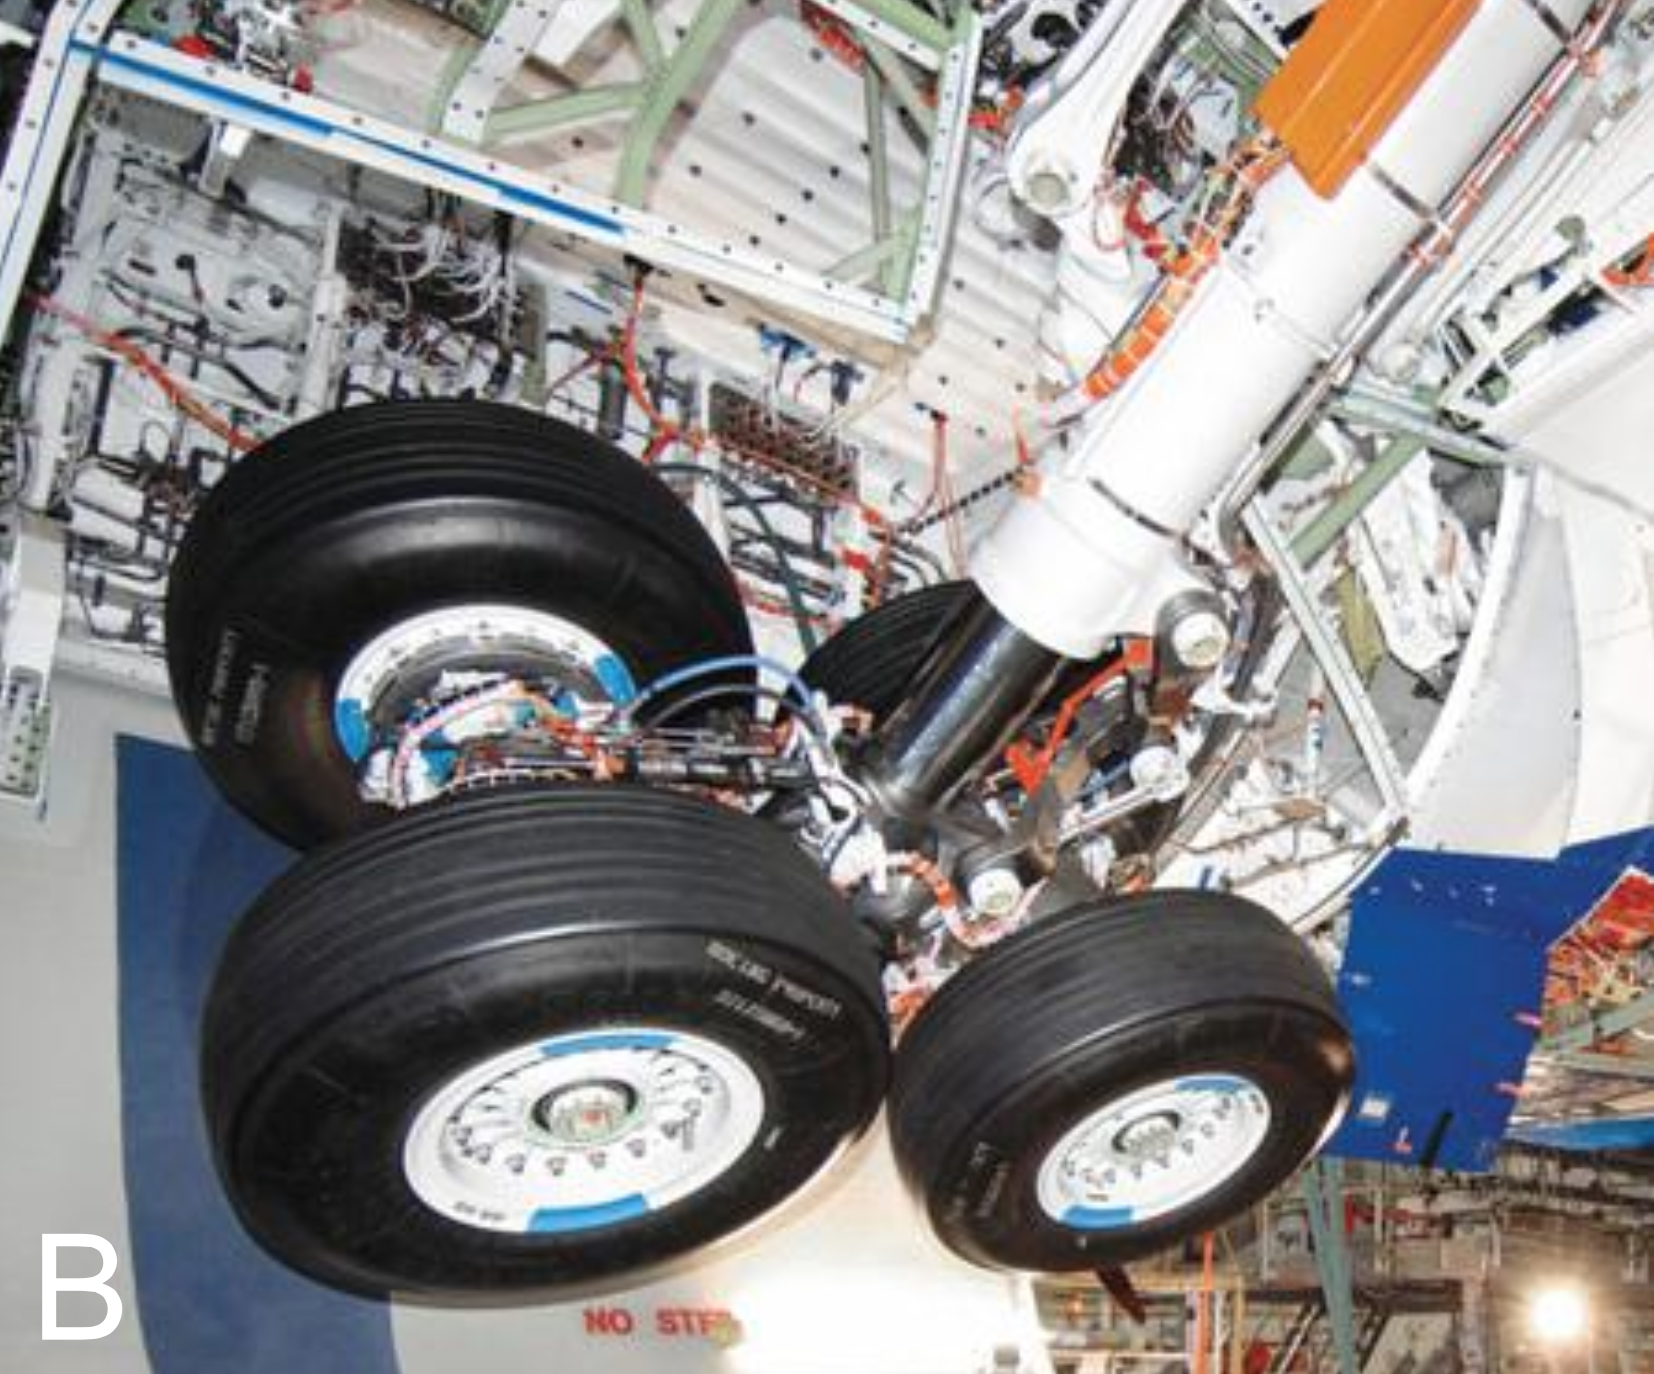
\includegraphics[width=0.4\textwidth]{figure/chap1/gear}}		\label{fig:plane gear}
%	\hspace{1cm}
%	\subfigure[飞机管路]{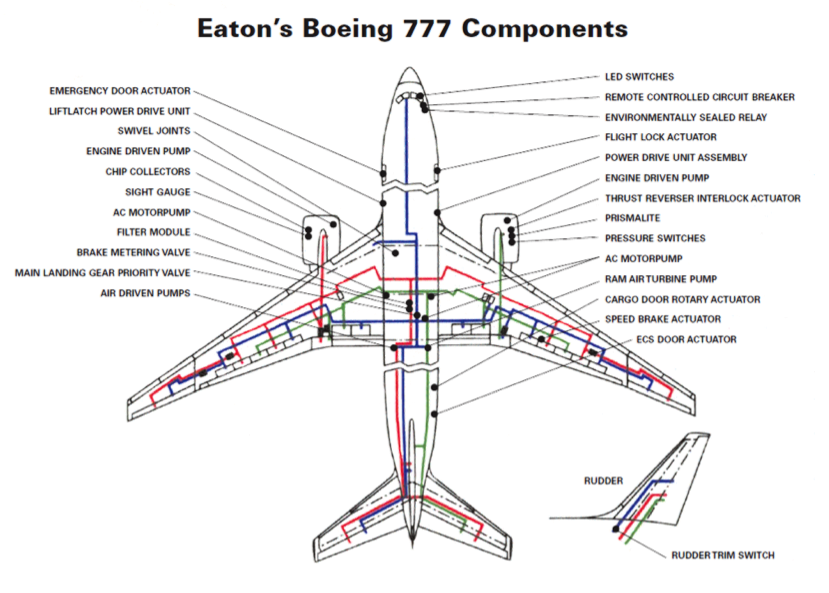
\includegraphics[width=0.5\textwidth]{figure/chap1/Plane}}    \label{fig:plane}
	\subfigure[机身软管管路(a.软管,b.液压源)]{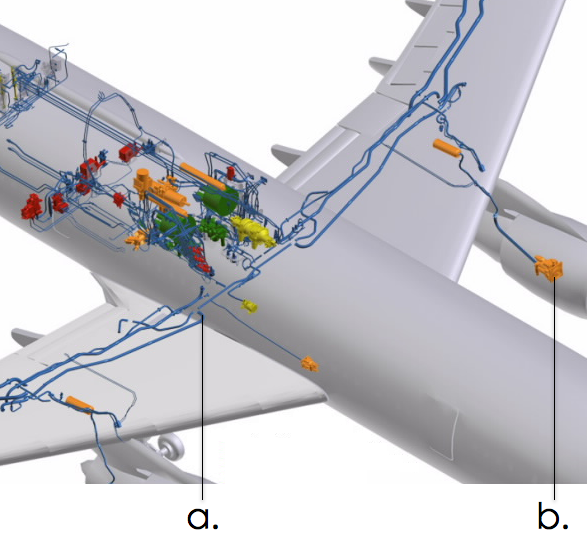
\includegraphics[width=0.4\textwidth]{figure/chap1/plane-cruit}}    \label{fig:plane-cruit}
	\hspace{1cm}
	\subfigure[发动机软管管路(a.软管,b.液压源)]{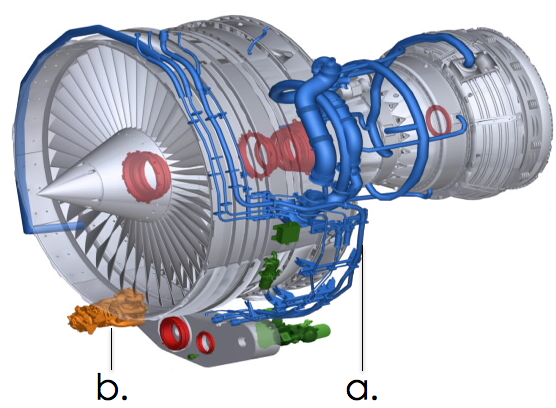
\includegraphics[width=0.4\textwidth]{figure/chap1/engine-cruit}}    \label{fig:engine-cruit}
	\bicaption[fig:SRR]{这里将出现在插图索引中}{飞行器软管组件分布}{Fig}{Distribution of hose assembly in a plane}  \label{fig:plane-hose}
\end{figure}


%软管优势



%不同软管型号
软管组件根据不同的口径、编织加强层的层数、重量等参数有以下分类方法:重型、中型、轻型;低压、中压、高压。
重型管管径一般达到20mm,轻型管管径一般在10mm以下;
高压管一般爆破压力要求达到\SI{80}{\mega\pascal},低压管爆破压力一般在40MPa以下。
不同型号的软管对于着不同的工作环境,如以下表\ref{tab:hosefixposition}所示,




\begin{table}[!htbp]
	\centering
	\bicaption[tab:hosefixposition]{testtest}{不同型号软管组件安装位置}{Fig}{Position}
		
	\begin{tabular}{ccc}
		\toprule
		&    轻型     &     重型     \\ \hline
		低压 & 汽车刹车、转向传动 &  输运水、气  \\
		高压 & 飞机起落架、襟翼  & 飞机、船舶液压泵出口 \\ 
		\bottomrule
	\end{tabular} 
\end{table}

%解释表格
飞机、船舶液压泵出口处压强高,流量大,震动强,工作环境极为恶劣,因此国内外一般都采用重型高压软管组件,技术也都已经较为成熟。
飞机起落架、襟翼等部位处于机身液压系统的末端,但压强仍然很高,而且软管的安装空间很小,要求软管组件具有较小的弯曲半径。保持较高的爆破压力的同时,使得软管组件小型化、轻型化,这就对软管组件的设计水平提出了很高的要求。国外企业在轻型高压软管组件领域技术优势明显,基本垄断了该市场。

汽车领域也大量使用了软管组件,例如刹车制动管,转向传动管,空调管等。相比飞行器的液压系统,汽车的液压系统压强较低,如刹车制动管的爆破压力一般为35MPa至40MPa\footnote{GB 16897-2010}。但汽车行业对成本较为敏感,要求在保证设计指标的同时,使软管的结构达到最优化。这对软管的设计、制造也提出了很高的要求。

%软管材质
根据软管寿命、工作环境温度











编织加强层由编织机缠绕于内管之上:若干根金属纤维穿过编织机锭子合为一股,由锭子携带,在圆周上的相互穿插交叠形成编织层。
金属编织软管一般采用2×2的编织(twill)形式(如图 1(c)),这是因为金属纤维一般刚度较大,这种编织形式中每股纤维的曲率较小,可以减小金属纤维所受的应力。

 	 	 
					
\section{研究现状}

纤维编织加强软管的加工生产技术经过几次重大变革,至今为止,已经发展出了3代产品
%第一代
编织加强胶管

%第二代
金属增强软管组件是由美国发明并于上世纪60年代开始用于飞机的液压系统,到上世纪90年代中期,已经广泛应用于航空、航天领域。为此,美国建立了一系列的军用、宇航产品技术标准或规范,例如:MIL-H-25579E、SAE AS604、SAE AS614等。其产品的最高使用温度为232℃,最高工作压力已经达到56MPa。目前广泛应用于各种类型的飞机和导弹、运载火箭等,例如:F-16、F-22、波音客机等。
%第三代
近年来,随着航空航天事业的飞速发展,对为之配套的聚四氟乙烯软管组件也提出轻量化的要求,传统钢丝增强软管组件已不能满足航空航天的设计要求。为了解决这个问题,非金属增强软管组件得到了大力发展,以美国为例,Titeflex、Eaton及Parker等国际知名公司纷纷研制出了各自的非金属增强软管组件产品,并广泛应用在波音、空客和达索等公司的军用、民用飞机上。Parker公司在本世纪初推出了Stratoflex 3154、Stratoflex 3190、Stratoflex 3191和Stratoflex 3192四种型号的非金属编织增强软管组件(见图2),产品的编织增强层根据不同的耐压等级采用不同材料,最高性能产品为耐压等级满足SAE AS1975规范要求的Stratoflex 3154产品采用Kevlar编织,最高工作压力为4000psi(28MPa)。Titeflex及Eaton也紧随其后,推出了自己的非金属编织增强软管组件产品。Titeflex公司主要有TITEFLEX 500、TITEFLEX RA170和TITEFLEX R270三种产品(见图3),最高可满足SAE AS5951规范要求的5080psi(35MPa),产品同样也采用Kevlar编织;Eaton的非金属编织增强软管组件产品型号为AE319、AE334和AE355(见图4),可满足SAE AS5951规定的5080psi(35MPa)工作压力要求。



目前对金属编织加强软管的研究,多见于汽车工业中的中刹车管[2]、转向传动管[3]、空调管[4]等。对软管加强层理论的研究,基本使用通过加强层的总体的要是通过软管理论主要有两个分支[5]:一种是加强层含量较低,橡胶管起主要作用的软管,由Kuipers等人[6,7]提出并完善,适用于帘线加强的软管;另一种是编织加强层主要承力的软管,主要研究的是钢丝螺旋缠绕加强层。软管轴向受拉时,缠绕的金属丝会沿缠绕方向“流动”。编织加强层仅作为螺旋缠绕的一种特例:两层缠绕方向相反,且不允许“流动”的缠绕层[5]。
近20年对编织加强结构的研究主要集中在复合材料编织。复合材料纤维编织的与金属纤维编织的传力机制差别非常明[8]:复合材料纤维只承受单向应力;而金属编织层中的金属丝间的接触关系会直接影响编织层整体的传力,不能忽视。因此,并没有至今尚没有成熟、独立,考虑金属丝间接触关系的编织加强层理论。
有学者尝试用连续介质力学的基本理论推导编织层的本构,如Evans[5]编织层金属纤维侧向传力机制,Horgan等人[9]提出了纤维加强材料的应变能密度函数,国内学者计算了编织结构强度与突加荷载的情况[10,11]。但主流的研究办法还是结合实验,提出能够反映加强层力学行为的有限元模型。Wijaya[4]对包含软管各层材料及编织层的试件进行了压缩实验,认为金属编织层的应力应变关系是线性的,在软管整体动态特性的研究中取得了较好的效果。Cho[3]研究了编织层在扣压安装接头中的力学行为,结合压缩实验提出了弹塑性的本构模型,Rattensperger[8]同样针对压缩的过程,编织层厚度方向引入一组等效非线性弹簧,表征金属纤维间相互作用。
Hachemi[12]对编织层进行了拉伸试验,将复合材料编织中考虑材料非线性行为的特征单元法(首先由Reese[13]提出)引入金属编织层的研究,提出了能够反映编织结构编织角变化的本构模型。该模型将编织层简化两层Rebar单元,只在编织方向上有刚度。但该模型仍然没有考虑两层Rebar单元之间相互接触的关系。

\section{研究内容}
本研究实验表明,Hachemi[12]本构模型的非线性行为并不足够强,不能与本研究中的高压金属编织加强软管的拉伸实验结果相吻合。我们试图通过引入金属纤维间的接触关系来修正该理论与实验的差距。使得包括非线性段的实验结果都能够与修正后的理论值相吻合。
 

%%==================================================
%% chapter02.tex for TJU Master Thesis
%% based on CASthesis
%% modified by wei.jianwen@gmail.com
%% Encoding: UTF-8
%%==================================================

\chapter{软管组件的结构及参数}
\section{引~言}
软管组件经过了几十年的发展演进,经过了大量的研究和实践,已经形成了一系列设计使用的规范。本文第一章已经对软管组件的行业发展进行了简要的介绍,本章着重介绍软管组件的结构,以及加强层理论发展。

\section{软管组件结构}
软管组件,承压能力相对较强,远超普通胶管;结构如图\ref{fig:hose structure-1}所示,
由内管、加强层、金属连接件组成。根据不同的使用环境一般还有不同种类的保护层。



\begin{figure}[!htbp]
	\centering
	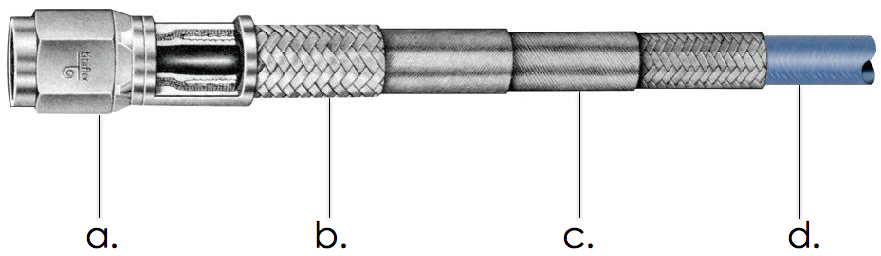
\includegraphics[width=0.6\linewidth]{figure/chap1/Hose-Structure}
	\fcaption{软管组件结构(a.接头,b.金属纤维编织层,c.金属纤维缠绕层,d.内管)}{Hose Structure(a.Coupling,b.Braid Layer,c.Helix-wound Layer,d.Inner Tube)}[软管组件结构]
	\label{fig:hose structure-1}
\end{figure}

\begin{figure}[!htbp]
	\centering
	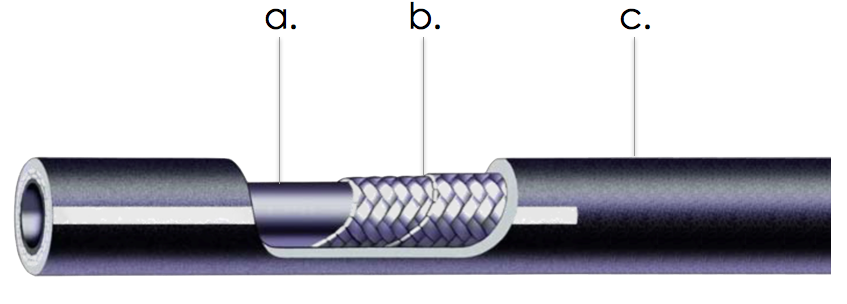
\includegraphics[width=0.6\linewidth]{figure/chap1/Parker-hose}
	\fcaption{软管组件结构(a.内管,b.金属纤维编织层,c.保护套)}{Hose Structure(a.Inner Tube ,b.Braid Layer,c.Coat Tube)}[软管组件结构]
	\label{fig:hose structure-2}
\end{figure}

\subsection{内管}


内管主要起到传输介质的作用,内管直接与油液接触,故要求在长期工作状态下不应受流体腐蚀,能防漏。主要选用的材质是塑料或者橡胶,例如:
\begin{inparaenum}
	\item 
	丁腈橡胶
	\item 
	氯丁橡胶
	\item 
	聚四氟乙烯等。
\end{inparaenum}		
其中,聚四氟乙烯又有“塑料王”之称,它重量轻、耐老化、耐热耐寒性好、抗腐蚀及化学稳定性好,在$ - 60 $\textcelsius \textasciitilde $ +250 $\textcelsius 温度下,可在一定半径范围内随意弯曲,耐疲劳性好,有较大的强度。所以,目前航空界已普遍将它代替传统橡胶内管。传统橡胶内管主要在汽车行业以及大型工程机械中使用。
	
影响性能的主要因素还有内胶层的硬度、厚度和永久变形量。
硬度和永久变形量对密封性能影响很大。
一般硬度高、压缩后的永久变形量小,密封性能则愈好。
一般是在70\textasciitilde 85邵氏硬度,压缩永久变形50\%时为最好。
内胶层厚度最好为1.5\textasciitilde 2.5mm,
厚会在扣压时增加其流动量,造成多余的胶在接头芯套与胶管的接触端面内堆积,减小流通截面;太薄会在扣压时被压裂。
同时内胶层壁厚均匀性也很重要。如果厚度不均,压缩后会造成一面裂断、一面堆胶。
内管表面出现的麻坑也是影响性能质量的重要因素。
	
	
内管成形也是生产软管组件的第一个步骤。以四氟塑料为例,采用的是推挤成形,设备如图\ref{fig:inner-tube-produce}所示。由进料口将粉状的聚四氟乙烯原料通过推挤设备,混料、压坯、推挤、烧结。设备经过合理整合后,控制推挤与烧结速度的配合,可以生产出光滑、均匀的内管,也可以实现大长度连续地生产。











\begin{figure}[!htbp]
	\centering
	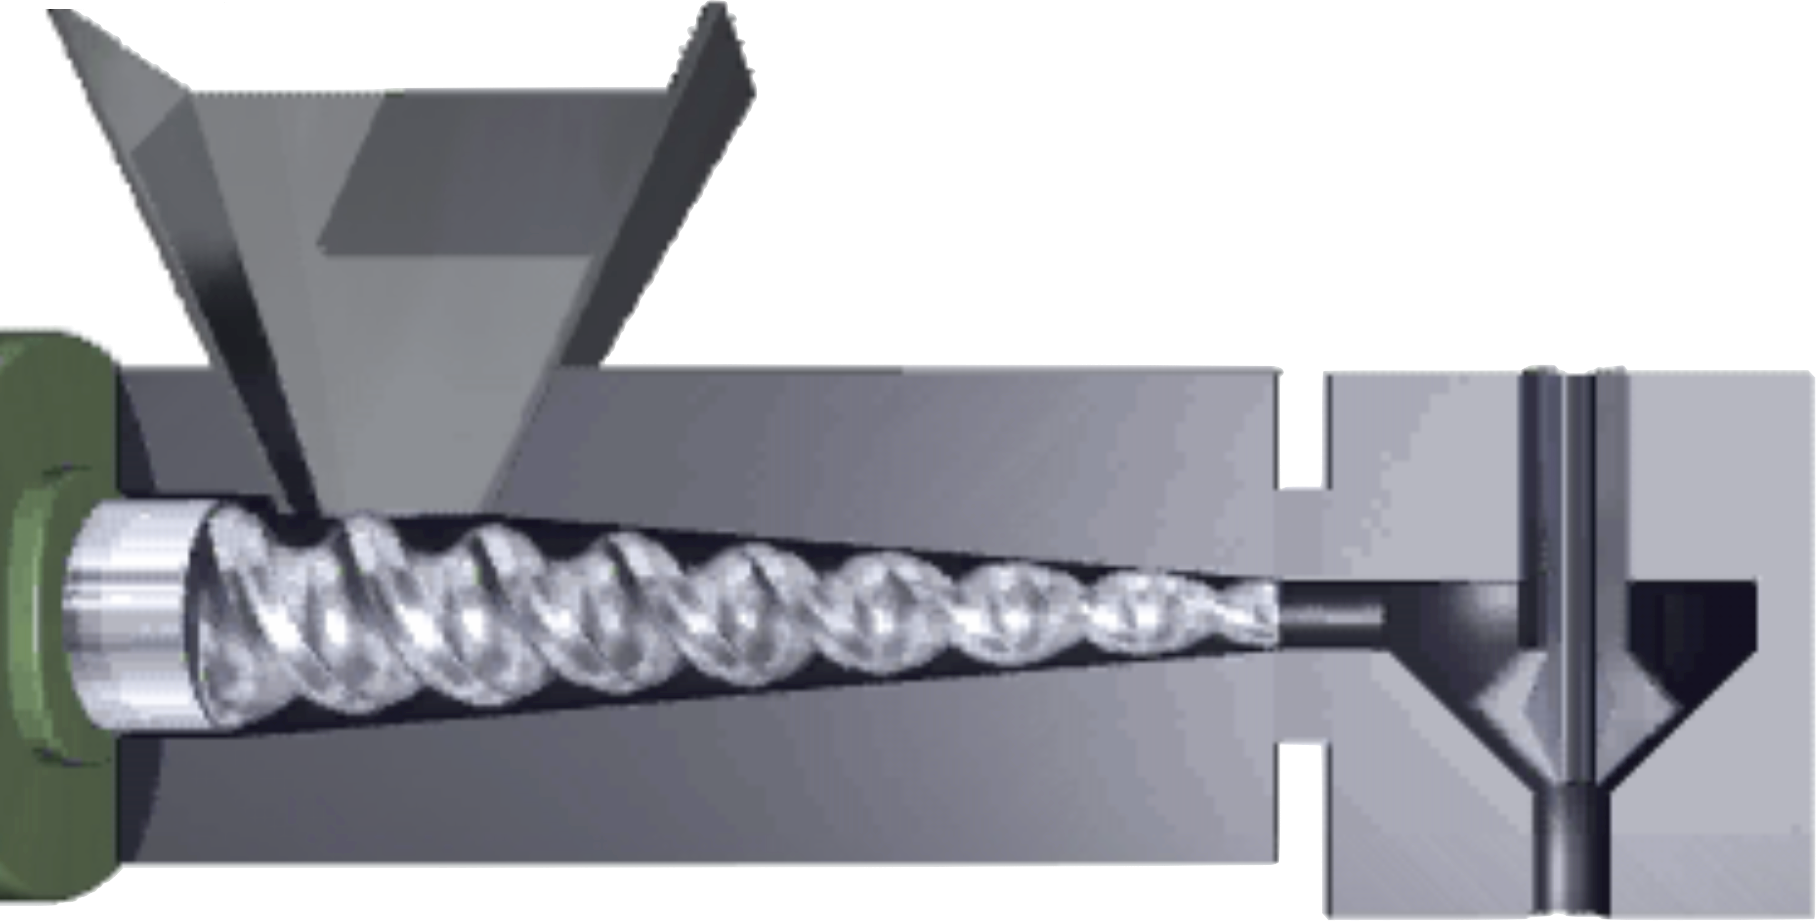
\includegraphics[width=0.4\linewidth]{figure/chap3/Hose/innertube-product}
	\fcaption{内管推挤成形}{inner tube}
	\label{fig:inner-tube-produce}
\end{figure}




\subsection{加强层}

内管成形冷却后就可以进入编织机或者缠绕机,为内管覆盖加强层。

编织机是生产软管组件的重要设备,如图\ref{fig:braider}所示。
编织机主要结构就是一个环形轨道,轨道上安装有两组锭子(spindle),
锭子由洪恩齿轮(Horn Gear)驱动,两组分别沿顺时针和逆时针方向,在圆周轨道上以类似三角函数图像的轨迹运动。
锭子携带若干根一股的金属纤维,使其相互上下交叠形成编织结构。
缠绕机机构与编织机结构相似,只是锭子固定在环形转盘上,随转盘在做圆周运动。

加强层的结构由几个参数控制:
\begin{inparaenum}[1).]
	\item 行程
	\item 编织角
	\item 编织层数。
\end{inparaenum}
这些参数是设计加强层的重中之重,具体在\ref{sec:parameter}节中讨论。

%编织机器图
\begin{figure}[!htbp]
	\centering
	\subfigure[]{
		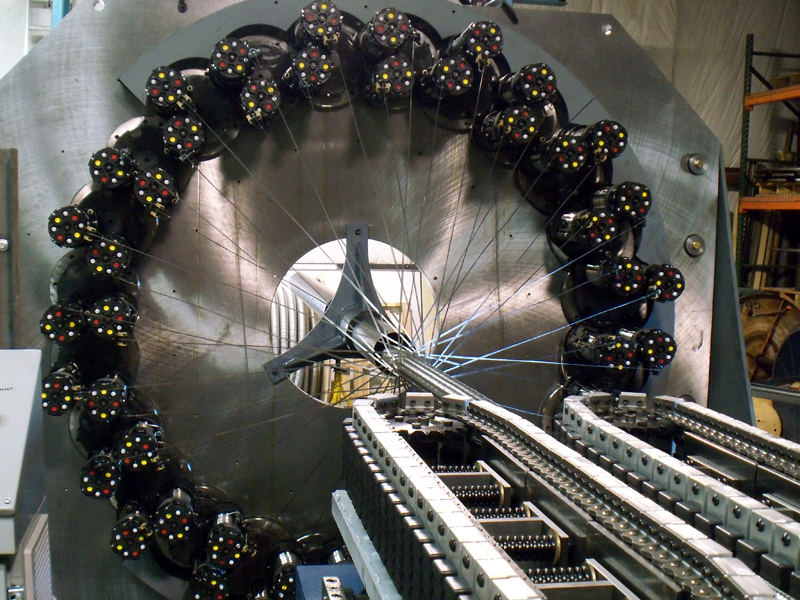
\includegraphics[width=0.4\linewidth]{figure/chap3/Hose/braider-1}}
	\hspace{1cm}
	\subfigure[]{
		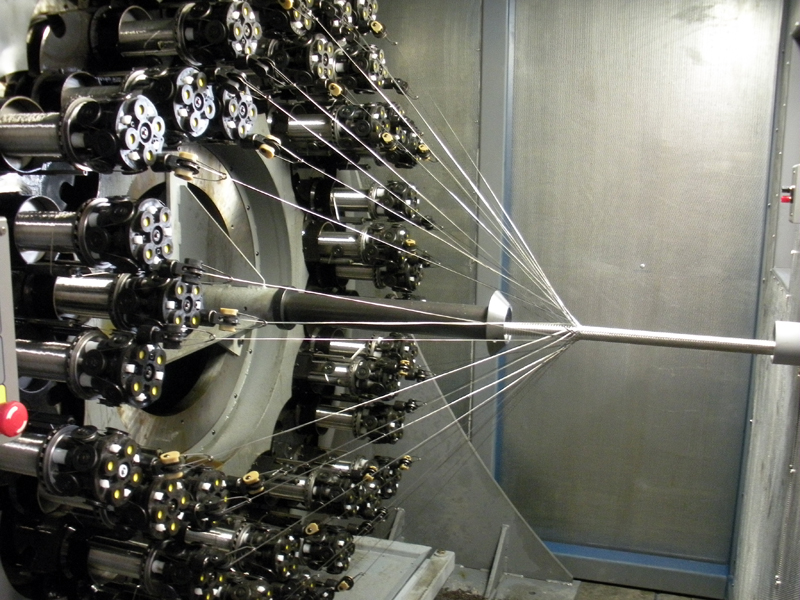
\includegraphics[width=0.4\linewidth]{figure/chap3/Hose/braider-2}}
	\subfigure[]{
		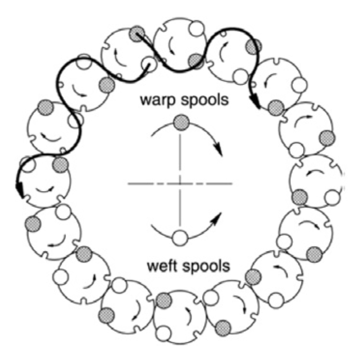
\includegraphics[width=0.3\linewidth]{figure/chap3/Hose/braider-theory}\label{fig:braider-theory-a}}
	\hspace{1cm}
	\subfigure[]{
		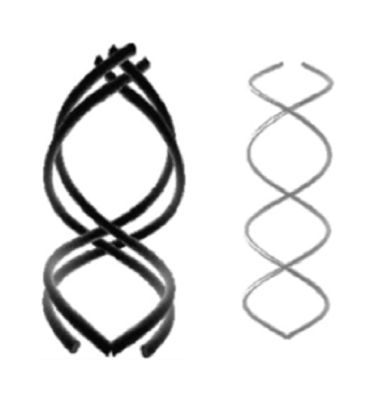
\includegraphics[width=0.3\linewidth]{figure/chap3/Hose/braider-theory-2}\label{fig:braider-theory-b}}
	\fcaption{编织机原理}{Braider}
	\label{fig:braider}
\end{figure}	

加强层是软管组件主要的承力结构,主要有编织和缠绕两种加强形式。对比两种加强层形式,各有优缺点。

缠绕层一般成对出现。所谓“成对”是指,缠绕加强时,不能只沿顺时针或逆时针方向缠绕,而必须反向的两层一组,来保持结构的受力平衡。
缠绕层中,金属纤维贴靠更为紧密,因而可以耐受更高的内压荷载,同时与内管贴合更好,不容易损伤内管。
另外缠绕层中的金属纤维弯曲半径较大,相互之间的接触关系较也相对比较简单,在两层之间有一般有中间胶,因此同一工作层的两层金属纤维之间没有交叉点。因而在承受动压时,不会因为金属纤维的交叉弯曲而产生应力集中或摩擦磨损。因此寿命要长于编织层,高频振动的环境优先选择缠绕加强。




但是缠绕层并不是一个稳定的结构,必须配合编织层,或者紧密贴合的橡胶套管,如\ref{fig:helix-tube-example}所示。因此缠绕加强一般比较笨重,多用于重型软管组件。


\begin{figure}[!htbp]
	\centering
	\subfigure[]{
		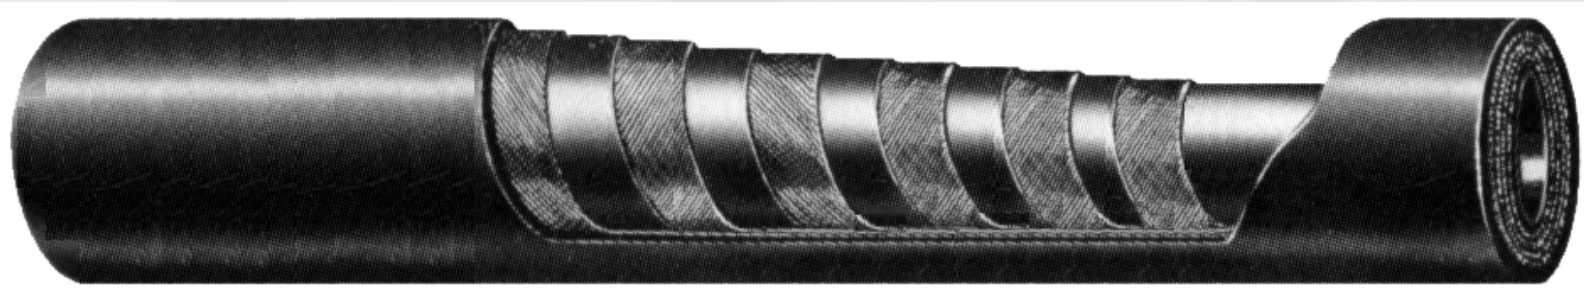
\includegraphics[width=0.45\linewidth]{figure/chap3/Hose/helix}\label{fig:helix-tube-example}}
	\hspace{1cm}
	\subfigure[]{
		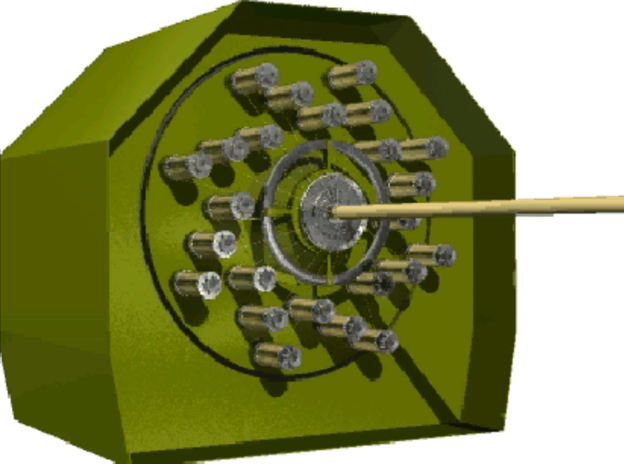
\includegraphics[width=0.3\linewidth]{figure/chap3/Hose/helix-wounder}\label{fig:helix-wounder}}
	\fcaption{缠绕机}{ Helix-wounding Machine}
	\label{fig:helix-tube}
\end{figure}


编织层中,纤维穿插交织形成了一个稳定的结构。一层编织相当于两层缠绕。由于同一编织层内钢丝之间的相互接触,在承受动压时,会因各自伸缩不一而造成钢丝相互之间的磨擦而影响其耐久性。
但是编织层自身就能形成稳定的加强结构,不需要其他结构辅助,非常轻巧。因此在轻型高压的软管组件中,必须使用编织层。



	
	
%\subsection{金属连接件}
%	\begin{asparaenum}
%		\item 扣压式\\
%		依靠接头公装的塑性变形和摩擦力形成有效连接。
%		\item 分离式\\
%		编织层覆盖系数小于缠绕曾,结构稳定,弯曲性能稳定,不会松散。
%		
%		\ref{fig:placeholder}
%		\ref{fig:placeholder:a}
%		\begin{figure}[!htbp]
%			\centering
%			\subfigure[]{\label{fig:placeholder:a}
%				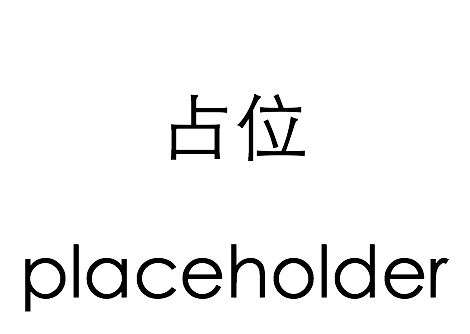
\includegraphics[width=0.4\linewidth]{figure/placeholder}}
%			\hspace{1cm}
%			\subfigure[]{
%				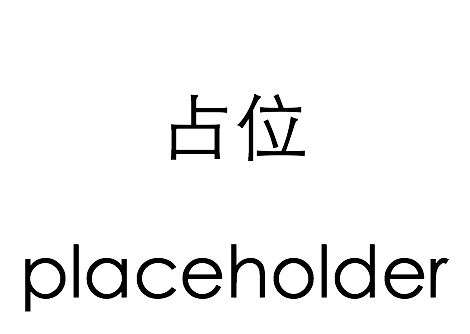
\includegraphics[width=0.4\linewidth]{figure/placeholder}}
%			\fcaption{占位图}{placeHolder}
%			\label{fig:placeholder}
%		\end{figure}
%	\end{asparaenum}	
	





	




\section{软管组件加强层参数}
\label{sec:parameter}
\subsection{编织角}



编织角针对编织加强层,缠绕角针对缠绕编织层。
编织角指的是编织层中,纤维偏离软管轴向的角度;而缠绕角定义相同,因此本文统一称为编织角,指代加强层中纤维布置的角度(Lay Angle)。

\begin{figure*}[!htb]
\centering
\subfigure[]{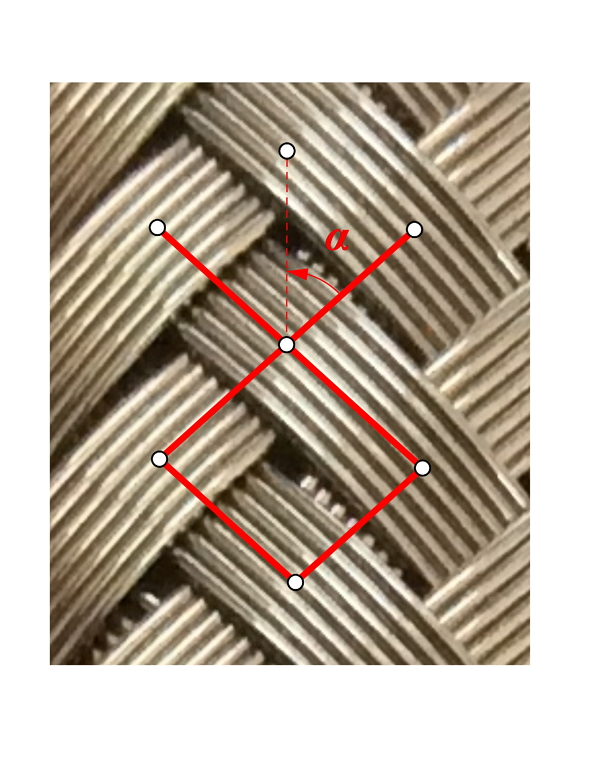
\includegraphics[height=0.2\textheight]{figure/chap2/braid-angle}
	\label{fig:braid-angle}}
\subfigure[]{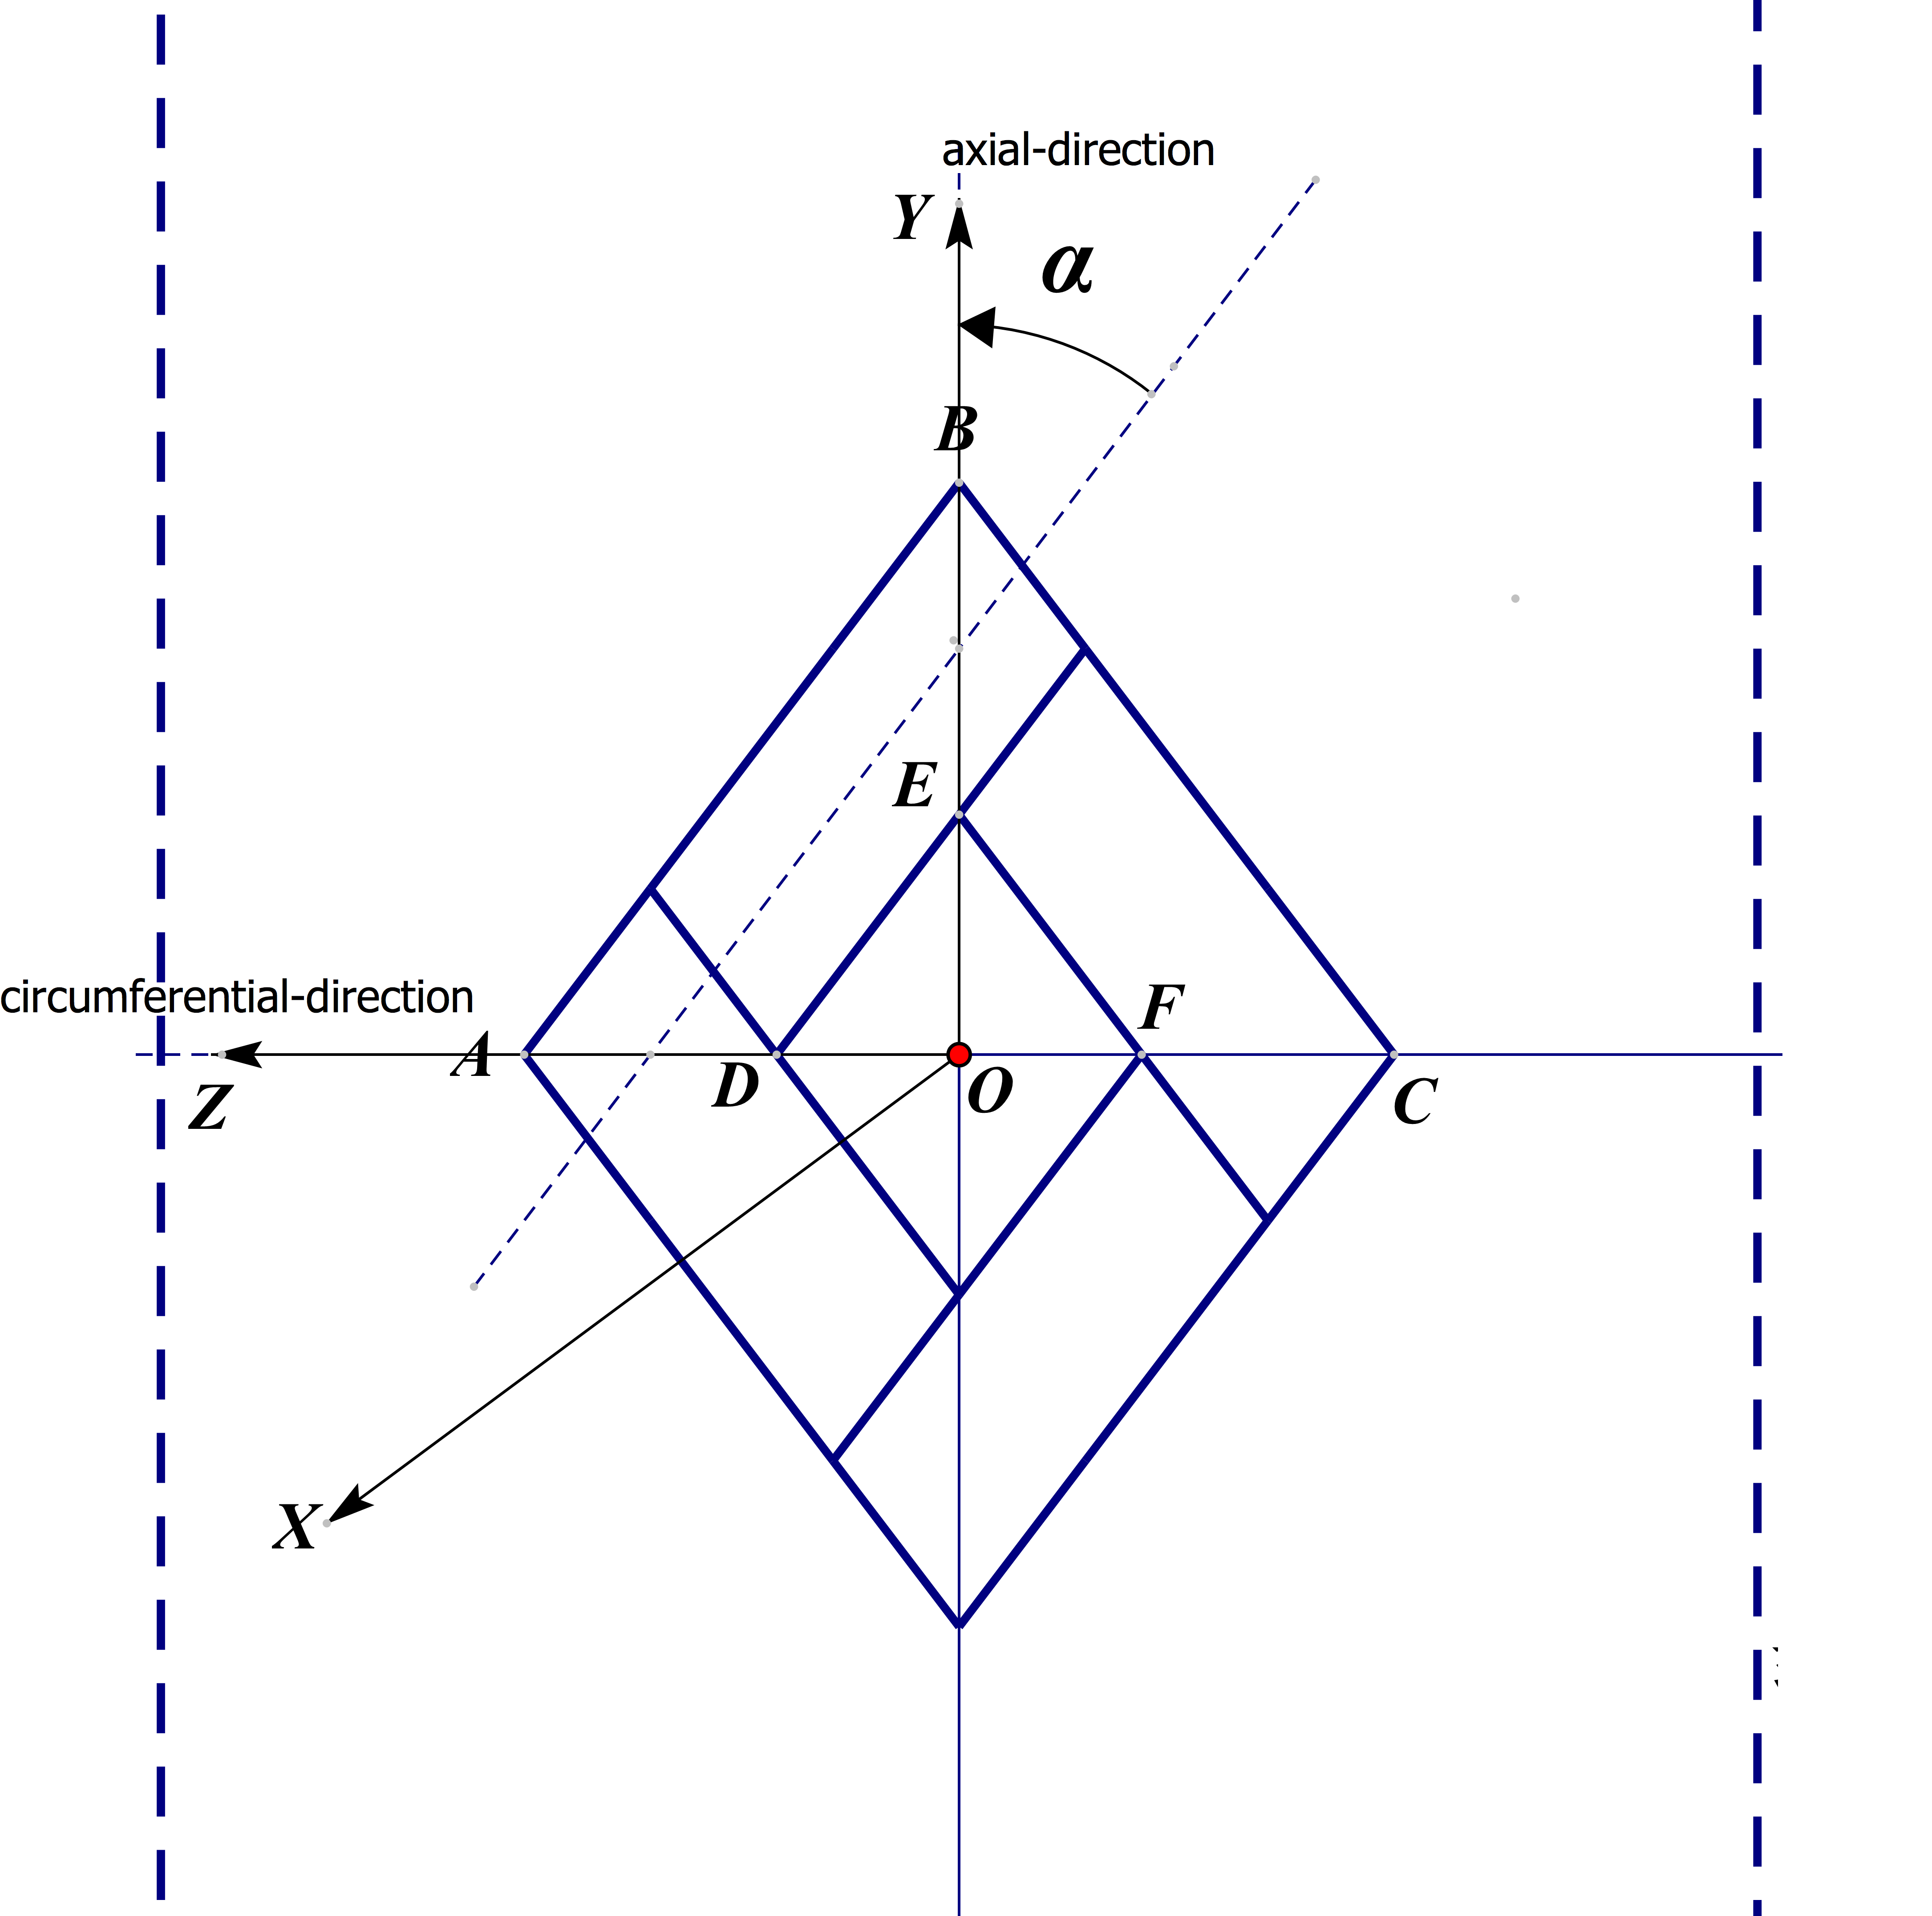
\includegraphics[height=0.2\textheight]{figure/chap2/braid-angle-2}
\label{fig:braid-angle-2}}
\subfigure[]{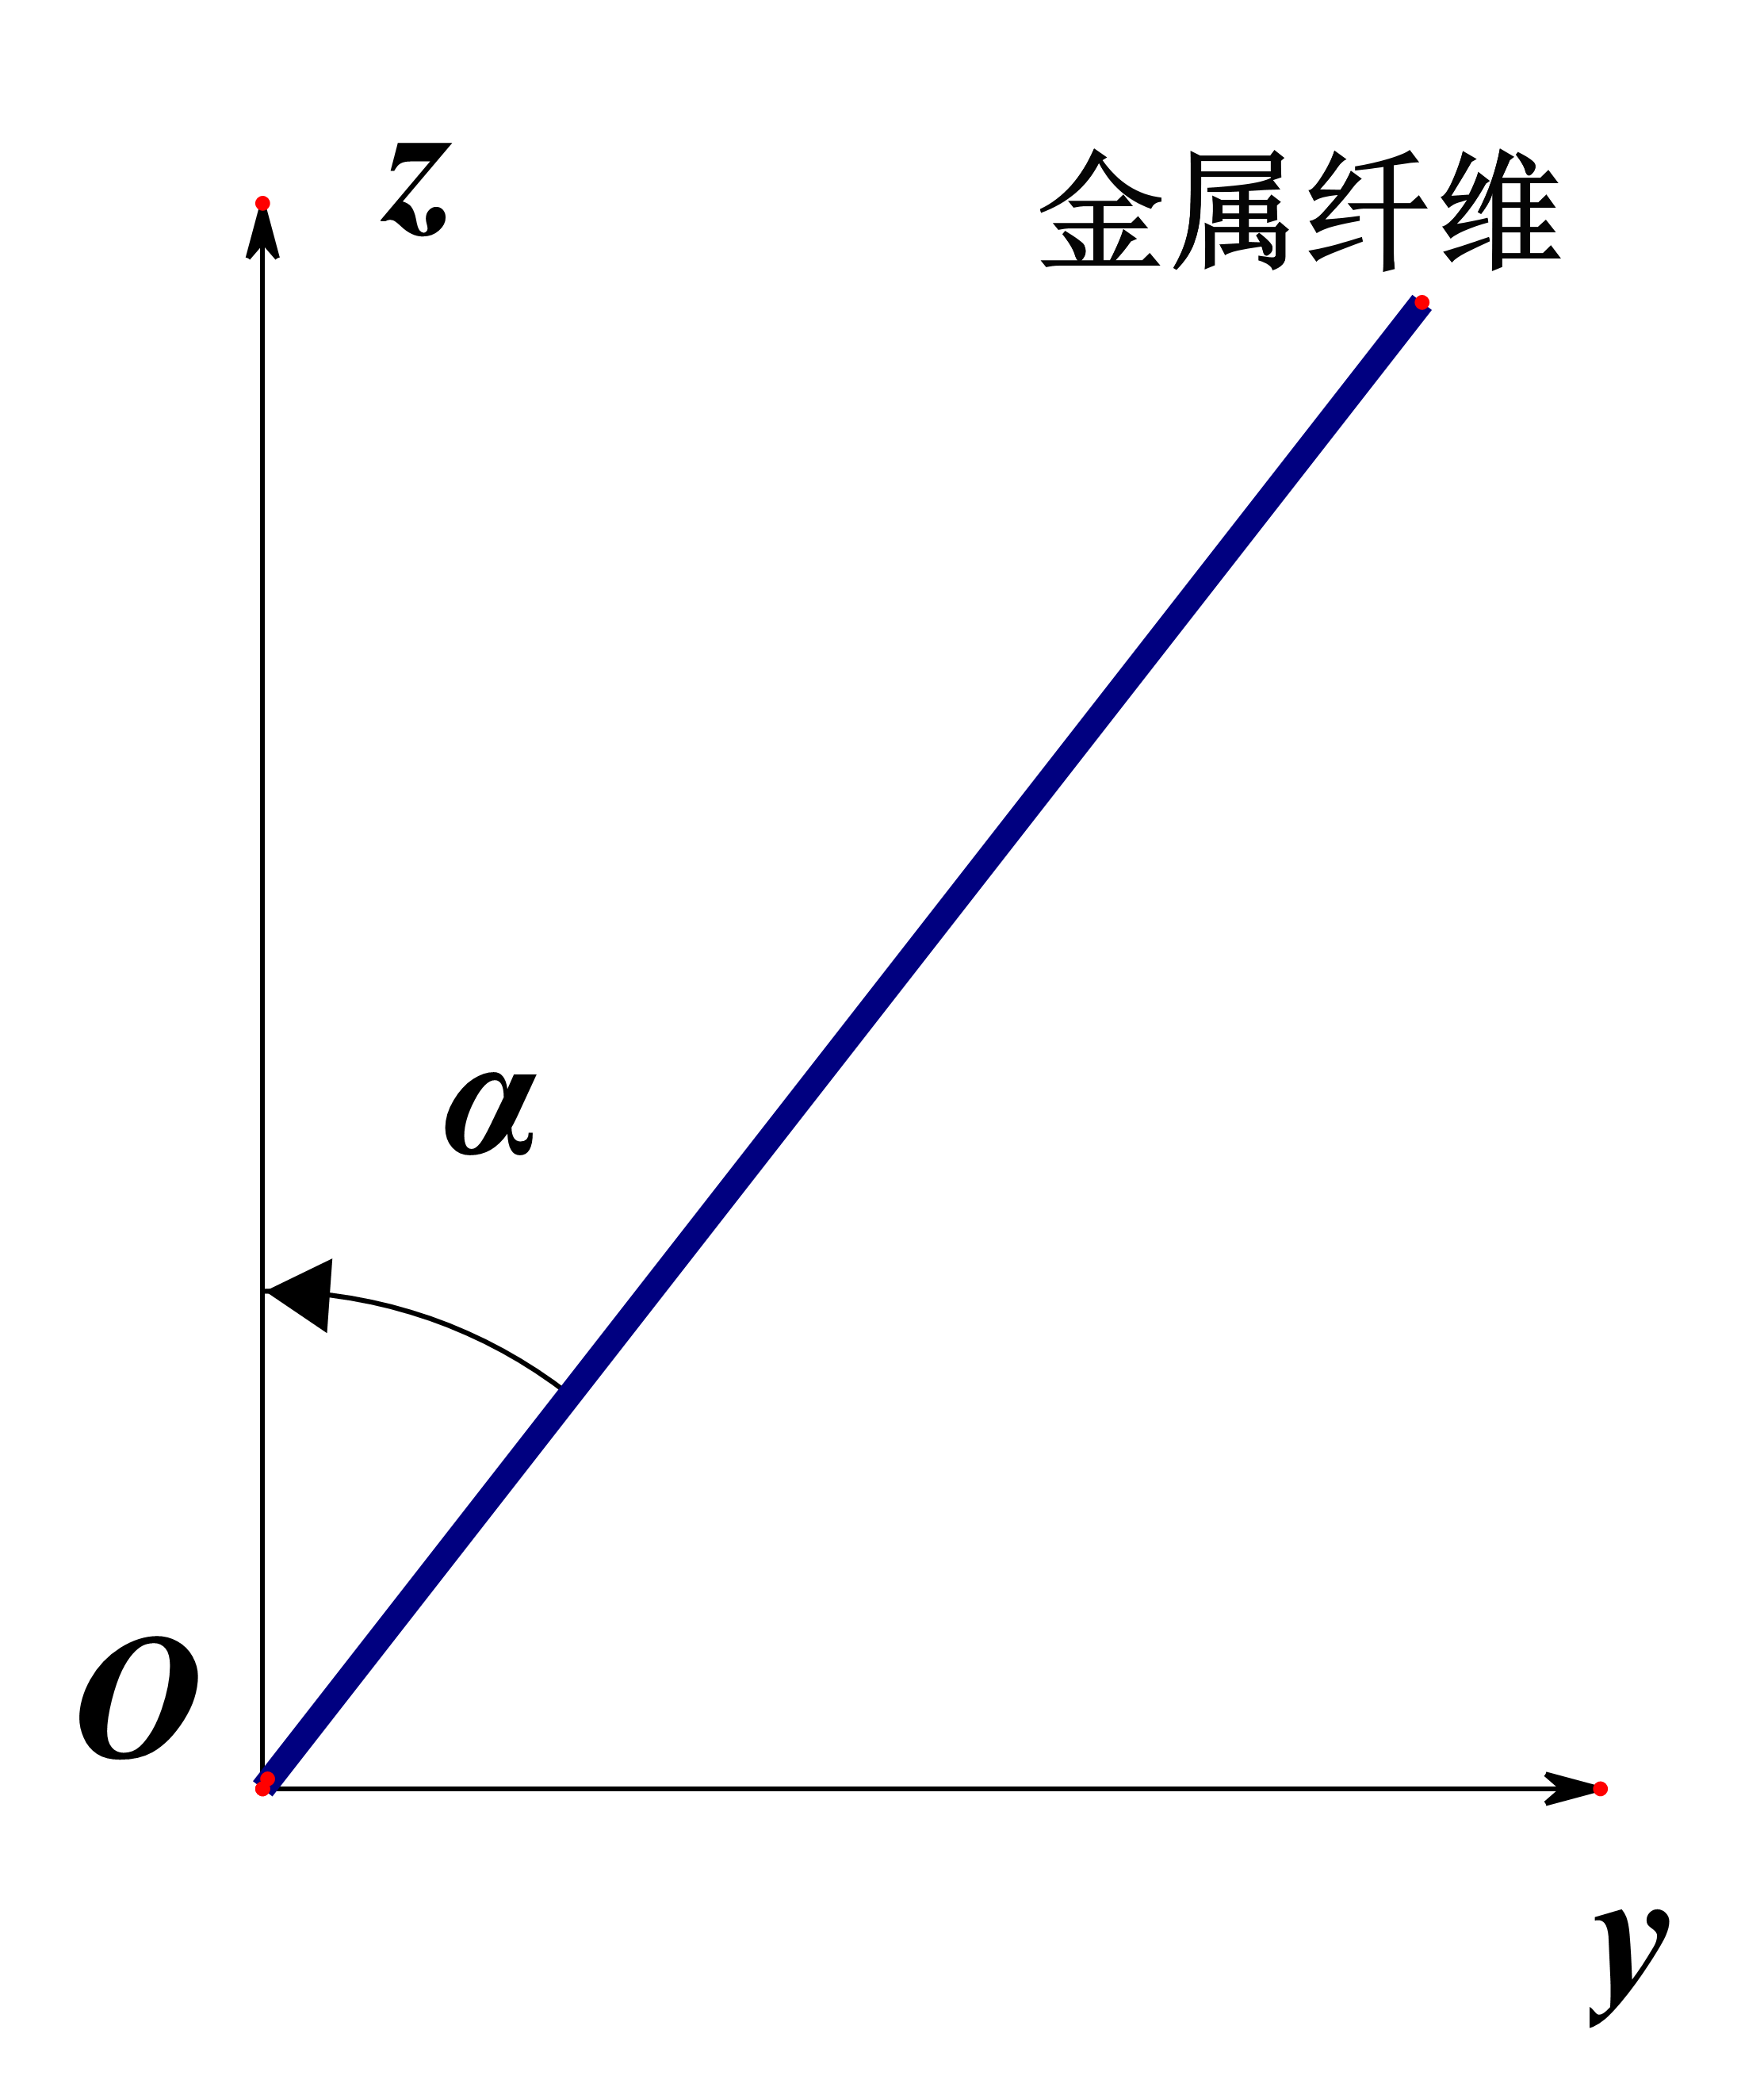
\includegraphics[height=0.2\textheight]{figure/chap2/braid-angle-3}
\label{fig:braid-angle-3}}
\fcaption{编织角及特征单元}{Braid angle and representive cell}
\label{fig:braid angle and represtive cell}
\end{figure*}


编织角是设计加强层时最重要的参数,以此确定编织机编制的螺距。
目前软管组件的编织层一般将编织角设定为平衡角。





\subsection{编织密度}

缠绕层中的加强纤维可以相互紧靠,而编织层中每股纤维中间会留下空隙,如如图\ref{fig:braid-angle-2}所示,为编织层的特征单元。特征单元在软管环向包含2股纤维,则特征单元的宽度为:

\begin{equation}
\frac{{\pi D}}{{{N_S}/2}} = \frac{{2\pi D}}{{{N_S}}}
\end{equation}

则特征单元中ABC区域的面积$ S_{ABC} $为:
\begin{equation}
\frac{1}{2}\left( {\frac{{2\pi D}}{{{N_S}}}} \right)\left( {\frac{{2\pi D}}{{2{N_S}\tan \alpha }}} \right) = {\frac{{{\pi ^2}D}}{{{N_C}^2\tan \alpha }}^2}
\end{equation}


空隙DEF区域面积$ S_{DEF} $为:
\begin{equation}
\label{eq:area-of-gaps}
S_{DEF}=\frac{1}{2}{\left( {\frac{{2\pi D}}{{{N_S}}} - 2\frac{W}{{2\cos \alpha }}} \right)^2}\frac{1}{{\tan \alpha }}
\end{equation}


其中,$ W = {N_W}\phi  $,为一股纤维的宽度。
则纤维覆盖的比例为$ 1 - \frac{{{S_{ABC}}}}{{{S_{DEF}}}} $


\begin{equation}
\xi_{lateral} = 1 - {\left( {1 - \frac{{{N_C}{N_W}\phi }}{{2\pi D\cos \alpha }}} \right)^2}
\end{equation}

这个比例$ \xi_{lateral}  $一般称为编织层覆盖系数(cover factor),也成为侧向编织密度,用于描述编织层编织的紧密程度。



若编织层采用金属纤维,纤维不能填满编织层占据的空间,进而有了截面编织密度$ \xi_{section} $的概念。编织层所有纤维的截面面积为:

\begin{equation}
{N_S}{N_W}\frac{{\pi {\phi ^2}}}{4}
\end{equation}

编织层占据的空间的截面积为:

\begin{equation}
\frac{\pi }{4}\cdot({D^2} - {D_{tube}}^2)
\end{equation}

其中,$ \phi $为 单根纤维的直径,$ D $为编织层外径,$ D_{tube} $为内管覆盖编织后的外径。由于编织机在编织过程中内管会被压缩,一般很难确定编织完成后得内管的外径;单层编织层理论上相当于两层金属纤维,但编织层的厚度一般大于两层。不妨设编织层的厚度为$ \tau\phi $,其中$ \tau $为编织层厚度与单根金属纤维比值,一般$ \tau  \in \left[ {2,5} \right]$。


\begin{equation}
\label{eq:section-epsilon}
{\xi _{section}} = \frac{{{N_S}{N_W}\frac{{{\phi ^2}}}{{\cos \alpha }}}}{{{D^2} - {{\left( {D - \tau \phi } \right)}^2}}} = \frac{{{N_S}{N_W}\phi }}{{\tau  \cdot \cos \alpha (2D - \tau \phi )}}
\end{equation}

由于$ \tau $值很难确定,工业中一般选择将侧向编织密度$ \xi_{lateral} $作为定义软管组件编织层编织密度的方法。


%\subsection{编织层数}






\section{软管组件性能参数}

软管组件主要包括一下几个重要的参数:
\begin{compactenum}
	\item 最大工作压力\\
	胶管在使用时所能承受的最大压力包括瞬间的峰值压力
	\item 试验压力\\
	软管耐压试验使用的压力,通常是额定压力的2倍
	\item 最小爆破压力\\
	使胶管破裂时所使用的真实压力,最小爆破压力通常是额定压力 的4倍
	\item 弯曲半径\\
	在不影响软管寿命的情况下软管所能弯曲的半径
	\item 长度变化\\
\end{compactenum}




\section{软管组件验证试验}
为了保证软管组件安全工作,美国、欧洲和国际标准都规定了一下几个重要的试验:
\begin{compactenum}
	\item 爆破试验\\
	以一定的升压速率,增加内压,直到软管组件发生渗漏、接头发生脱头或者管体破裂。以此时的压力值为软管组件的最小爆破压力。
	
%	\begin{figure}[!htbp]
%		\centering
%		\subfigure[]{
%			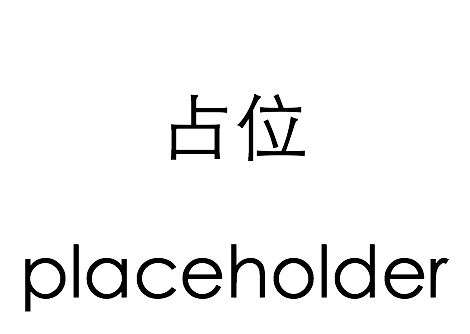
\includegraphics[width=0.4\linewidth]{figure/placeholder}}
%		\subfigure[]{
%			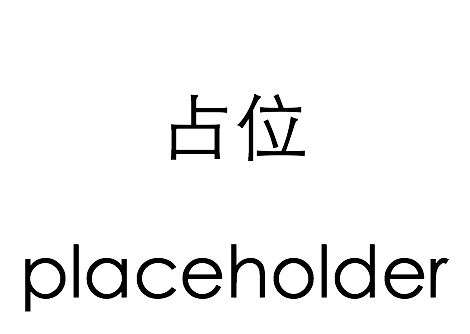
\includegraphics[width=0.4\linewidth]{figure/placeholder}}
%		\fcaption{占位图}{place holder}
%		\label{fig:placeholder}
%	\end{figure}
	
	\item 试验压力\\
	软管耐压试验使用的压力,通常是额定压力的2倍
	\item 脉冲试验\\
	按照规定压力、频率施加脉冲荷载,反复施加直到管体破坏。
\end{compactenum}	




%%==================================================
%% chapter03.tex for TJU Master Thesis
%% Encoding: UTF-8
%%==================================================

\chapter{软管组件加强层理论发展综述}


\section{引~言}


%目前对金属编织加强软管的研究,多见于汽车工业中的中刹车管[2]、转向传动管[3]、空调管[4] 等。

软管组件作为一种上世纪中叶,就开始广泛使用的重要工业构件,
事实上,对其的研究一直以实验、实用为主,没有形成一套通用完整的体系。图\ref{fig:hose-system-theories}描述了软管组件的理论路线和分支。

\begin{figure}[!htbp]
\centering
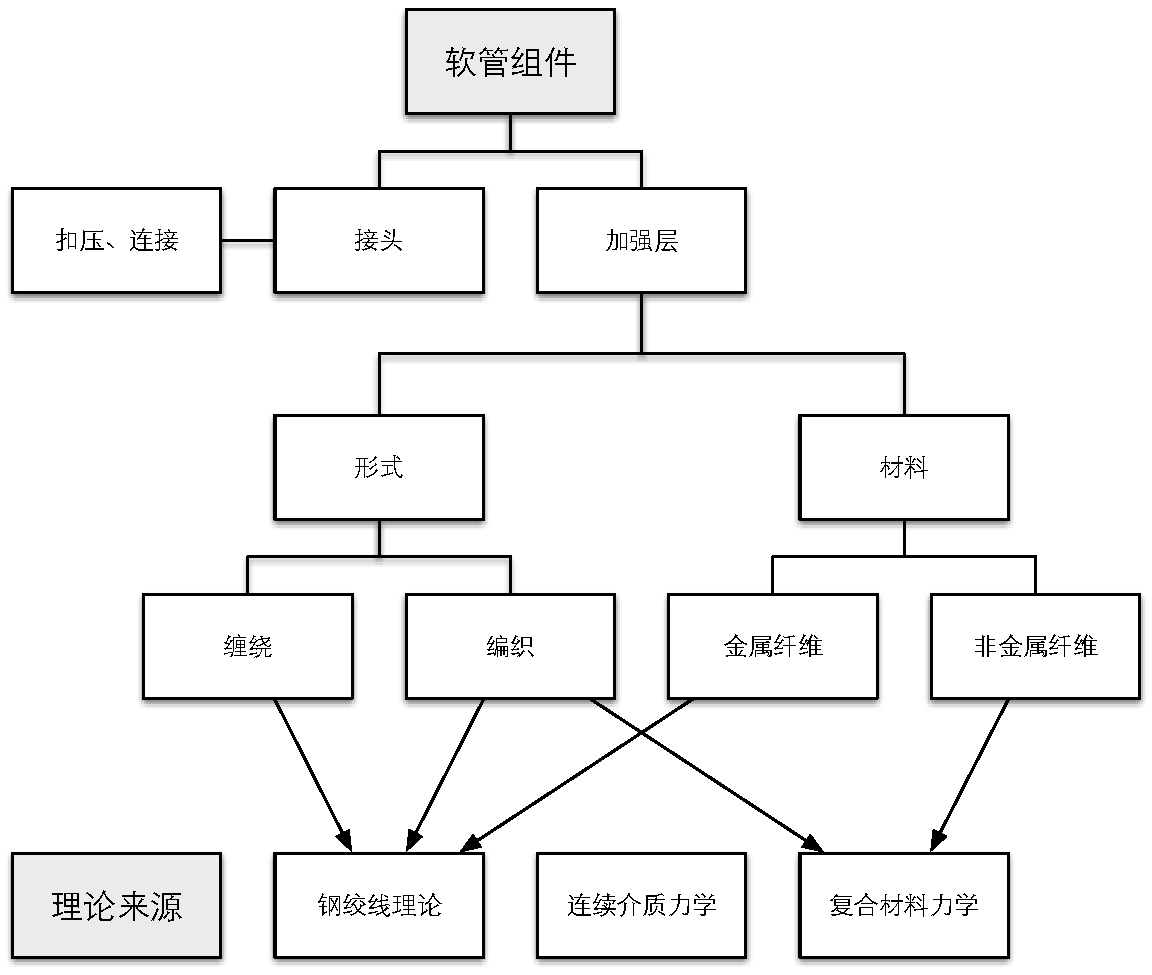
\includegraphics[width=0.7\linewidth]{figure/chap3/理论体系}
	\bicaption[fig:theory-system]{软管组件理论体系}{软管组件理论体系}{Fig}{Hose Assembly Theory Branches}
	\label{fig:hose-system-theories}
\end{figure}

软管组件的理论与研究首先分为两个对象:
\begin{inparaenum}[1).]
	\item 接头
	\item 加强层。
\end{inparaenum}
本文的研究主要针对加强层,这里不对软管组件的连接技术进行阐述。而加强层包含了缠绕、编织两种形式,又包括了金属纤维、非金属纤维两种材料,理论界并没有明确和统一的认识,而是基于各自不同的理论之上。

加强层的理论研究成果,主要是建立在三个理论体系之上的,包括了
\begin{inparaenum}[1).]
	\item 钢绞线理论
	\item 复合材料力学
	\item 连续介质力学
\end{inparaenum}



\section{理论分支概述}
钢绞线理论,来源于悬索、电缆等结构。钢绞线理论应用于加强层的力学分析,有两个主要的分支\cite{Evans2002}:
\begin{inparaenum}[1).]
	\item 加强层含量较低,橡胶管起主要作用的软管,由\citeauthor{Kuipers1989}等人[6,7]提出并完善,适用于帘线加强的软管;
	\item 加强层主要承力的软管,主要研究的是高密度钢丝缠绕加强层。
\end{inparaenum}
这套理论体系成熟与上世纪90年代初,适用于金属纤维的缠绕层,编织层一般作为缠绕层的一种扭转为0的特殊情况。前文提到的第一代、第二代软管组件一般是以这套理论指导设计的。

随着第三代非金属加强软管组件的大量使用,近20年来,对编织加强结构的研究主要集中在复合材料编织。复合材料纤维编织的与金属纤维编织的传力机制差别非常明显[8],研究方法的也有所区别:钢绞线理论一般以钢丝为载体;复合材料一般采用特征元法作为力学分析的对象。复合材料理论中有大量简化编织结构的理论,许多学者选择其中适合软管加强层的理论开展了工作



也有学者尝试用连续介质力学的基本理论推导编织层的本构,\citeauthor{Horgan2005}\cite{Horgan2005} 提出了纤维加强材料的应变能密度函数,
国内学者计算了编织结构强度与突加荷载的情况\cite{2009b}。

但是,主流的研究办法还是结合实验,提出能够反映加强层力学行为的有限元模型。\citeauthor{Wijaya2012}\cite{Wijaya2012}对包含软管各层材料及编织层的试件进行了压缩实验,认为金属编织层的应力应变关系是线性的,在软管整体动态特性的研究中取得了较好的效果。\citeauthor{Cho2005}\cite{Cho2005}研究了编织层在扣压安装接头中的力学行为,结合压缩实验提出了弹塑性的本构模型,\citeauthor{Rattensperger2003}\cite{Rattensperger2003}同样针对压缩的过程,编织层厚度方向引入一组等效非线性弹簧,表征金属纤维间相互作用。



\section{基于钢绞线理论的研究}


%stepI hruska 
\citeauthor{hruska1951calculation}\cite{hruska1951calculation,hruska1952radial,hruska1953tangential}分析了钢绞线结构中一层钢丝的轴向、切向以及径向的应力。钢绞线中一层钢丝实际上就是一层螺旋缠绕结构,也被用于早期设计软管组件缠绕层的参考依据。而其理论并没有考虑结构半径的变化,也没有考虑钢绞线排布的角度$ \alpha_i $的变化。也就是说,该理论不能考虑编织层受内压后,结构的几何变化。该理论仅考虑了钢绞线的拉伸刚度,扭转和弯曲的刚度皆为0。钢绞线体系轴向拉力$ T_\alpha $与单根钢丝轴线拉力$ T_i $的关系为:
\begin{equation}
T_\alpha = T_i \cos{\alpha_i}
\end{equation}

1951年,\citeauthor{hruska1951calculation}也给出了单位长度径向力$ F_{RU} $与钢绞线拉力$ T $、钢丝曲率半径$ \rho $关系的表达式,如式\ref{eq:Hruska}所示。该理论提出时仅作为实验得到的经验公式,后在\citeyear{machida1973}由\citeauthor{machida1973}给出证明。

\begin{equation}\label{eq:Hruska}
{F_{RU}} = \frac{T}{\rho }
\end{equation}
其中,钢丝的曲率半径可以由螺旋缠绕的结构参数表征
\begin{equation}
\rho  = \frac{R}{{{{\sin }^2}{\alpha _i}}}
\end{equation}
$ R_i $为钢绞线总体半径。


1977年,\citeauthor{Entwistle1977}\cite{Entwistle1977}针对编织加强软管,提出了一套更为准确的理论假设。这套理论相对之前的理论,可以考虑缠绕层受内压荷载后,结构的几何变化。\citeauthor{Entwistle1977}对加强层几何变化的假设如图\ref{fig:assumption-deformed-geometry}所示,该理论不允许软管发生扭转,这是考虑到在该理论体系下编织层的扭转必须为0。

加强层变形前后的半径为$ R_i $、$ R_i' $,缠绕角为$ \alpha_i$ 、 $\alpha_i' $,钢丝应变为$ \varepsilon_i $,之间的关系可以通过图\ref{fig:assumption-deformed-geometry}中的几何关系表示

\begin{equation}
\frac{{{R_i}'}}{{{R_i}}} = \left( {1 + {\varepsilon _i}} \right)\frac{{\sin {\alpha _i}'}}{{\sin {\alpha _i}}}
\end{equation}

\begin{figure}[!htbp]
	\centering
		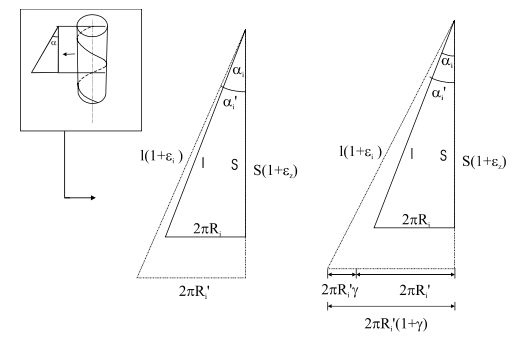
\includegraphics[width=0.7\linewidth]{figure/chap3/review/a}
	\bicaption[fig:assumption-deformed-geometry]{加强层几何变化假设}{加强层几何变化假设}{Fig}{Assumption for the deformed reinforcement geometry}
	\label{fig:assumption-deformed-geometry}
\end{figure}

1979年,\citeauthor{Knapp1979}\cite{Knapp1979}针对内芯可压缩的钢绞线结构进行了研究,采用了和\citeauthor{machida1973}(\citeyear{machida1973})相似的手段,引入了扭转因子$ \gamma_i $(图\ref{fig:assumption-deformed-geometry}),其表达式为:
\begin{equation}
{R_i}' = {R_i}\frac{{\left( {1 + {\varepsilon _i}} \right)\sin {\alpha _i}'}}{{\left( {1 + {\gamma _i}} \right)\sin {\alpha _i}}}
\end{equation}



\section{基于复合复合材料理论的研究}

\section{本文研究思路}
%%==================================================
%% chapter03.tex for TJU Master Thesis
%% Encoding: UTF-8
%%==================================================

\chapter{软管模型修正}
%%==================================================
%% chapter03.tex for TJU Master Thesis
%% Encoding: UTF-8
%%==================================================

\chapter{编织层非线性修正理论}


\section{引言}

在上一章中,通过拉伸实验,对软管组件编织层的力学行为进行了研究,得到了不同规格金属纤维编织层拉伸的力位移曲线,也探索出了一套系统的实验方法,简便而准确。本章就立足于实验得到的数据,针对拉伸实验中力位移曲线出现的强烈的非线性,展开研究,并试图给出理论上的解释。


本文第三章中介绍了\ha 编织层的基本理论。同时进行数值仿真的试算,体现了该理论几个不足之处尚待改进:
\begin{compactitem}
	\item 仿真结果仅能符合拉伸力位移曲线的线性部分,非线性段不能吻合;
	\item 该理论不能用于三维有限元分析,只能进行轴对称问题的分析,因为其刚度矩阵缺少切向刚度。
	\item 该理论仅适用于拉伸实验,不能用于内压爆破实验的建模;
	\item 该理论没有提出合适的强度分析方法,不能验证编织层是否发生破坏。
\end{compactitem}

以上几点不足之处,导致该模型被没有广泛使用。拉伸实验一般只是作为软管组件验证力学特性辅助实验手段,而内压荷载是软管组件最为主要的受力状态。


本章首先利用“修正基体”的方法对特征单元的刚度矩阵进行了补充,使其能够满足三维有限元计算的需要。

其次,对\ha 模型编织角理论部分进行了修正,还提出了编织角加速系数$ k $的概念,并对其物理意义进行了讨论。

另外,\ha 模型中“特征单元”并没有考虑编织层中纤维的上下起伏,导致模型偏刚,影响到内压荷载的计算结果。这里对其进行了修正。

\newpage



\section{有限元试算试件}
本章将分析各种因素对编织层非线性行为的影响,将会反复利用有限元模型试算的结果与第四章的实验结果进行对比。为保证各组试算结果间的可比性,每次试算默认取第一次、第二次拉伸实验的两组试件的参数进行试算,其规格参数格如表\ref{tab:characteristics-of-hose-specimen}所示。


\begin{table}[!htb]
	\centering
	\tcaption{试算试件参数}{characteristics of hose specimen}
	\label{tab:characteristics-of-hose-specimen}
	\begin{tabular}{@{\extracolsep{\fill}}>{\hspace{0.5cm}}cccc}
		\toprule
		                 &   试算试件-1    &   试算试件-2    &  \\ \midrule
		实验组别             &   拉伸实验-1    &   拉伸实验-2    &  \\
		试件原标号            &    芯棒-1     &   软管组件-2    &  \\
		软管形式             & 编织层  & 编织层+PTFE内管  &  \\
		编织层外径(mm)        &    7.60     &    7.70     &  \\
		内管内径(mm)         &    /     &    5.01     &  \\
		软管长度(mm)         &    320.0    &    421.5    &  \\
		编织角(\textdegree) &    52.1     &     52.4      &  \\
		股数$\times$根数     & 24$\times$6 & 24$\times$6 &  \\
		钢丝直径(mm)         &     0.2     &     0.2     &  \\
		拉伸量(mm)         &     80     &     160    &  \\
		 \bottomrule
	\end{tabular} 
\end{table}  

\newcommand{\shi}{试算试件-1}
\newcommand{\shii}{试算试件-2}


\section{修正基体理论}

Hachemi的理论将金属纤维简化为2D的特征单元,然后进行平均化得到特征单元的刚度矩阵。事实上这套理论只考虑了纤维本身的力学属性,如\ref{fig:modified-matrix-relation}所示,纤维间关系也是编织层力学特性的重要贡献部分,也是难点所在。

\begin{figure*}[!htb]
\centering
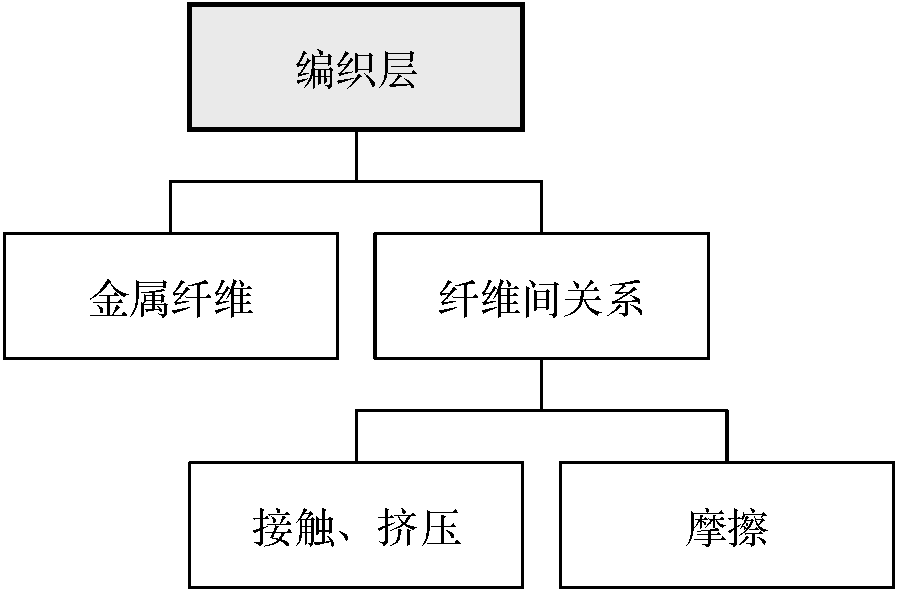
\includegraphics[height=0.2\textheight]{figure/chap5/modified-matrix-relation}
\fcaption{编织层本构关系的内容}{elements of the constitutive relation of braid reinforcement layer}
\label{fig:modified-matrix-relation}
\end{figure*}

编织层纤维简单接触、摩擦往往很难通过理论分析求得。而金属纤维的力学特性相对则是明确的。因此这里引入一种方法:修正基体法(Modified Matrix Method)。

修正基体法最初由\citeauthor{modmm1978}\cite{modmm1978}提出,利用平均化的观点提出来的。修正基体法一般将三维复合材料通过修正的基体模型简化成二维结构,,然后根据现有的理论计算二维编织材料的弹性模量。

尽管有所不同,还是可以利用这种思路,通过基体分担部分纤维的特性,在保留原有纤维理论体系的同时,引入新的纤维间的关系。

实际上编织层是没有基体的。非金属软管加强编织层一般也没有基体。但是纤维间的接触、摩擦对于编织层来说,是独立于纤维的力学特性之外的,起到的作用是稳定、限制结构,类似于基体的作用。那么不妨引入数学上假想的“基体”,对金属纤维本身计算的刚度矩阵进行修正,相当于将金属纤维的接触、摩擦等纤维间关系纳入了“基体”的体系,与纤维本身形成“复合材料”。修正基体可以弥补纤维本身计算的结果与编织层实际力学特性间的差距,起到修正的作用。

参考各向同性材料的刚度矩阵,

\begin{equation}
\label{eq:common-stifness}
\left[ {\begin{array}{*{20}{c}}
{2\mu  + \lambda }&\lambda &\lambda &0&0&0\\
\lambda &{2\mu  + \lambda }&\lambda &0&0&0\\
\lambda &\lambda &{2\mu  + \lambda }&0&0&0\\
0&0&0&\mu &0&0\\
0&0&0&0&\mu &0\\
0&0&0&0&0&\mu 
\end{array}} \right]
\end{equation}

其中, 
\begin{equation}
\mu  = \frac{E}{{2\left( {1 + \nu } \right)}}
\end{equation}

\begin{equation}
\lambda = \frac{{E\nu }}{{\left( {1 + \nu } \right)\left( {1 - 2\nu } \right)}}
\end{equation}


 $ {C_{{\rm{1111}}}} $可以表征两层金属纤维法向接触的刚度(如图 \ref{fig:modifiedmatrix}所示)。将复杂的多点接触的接触刚度简化为各向同性材料内部的弹性刚度,则:

\begin{equation}
{C_{{\rm{1111}}}}{\rm{ = }}\xi E
\end{equation}


$  {C_{{\rm{1212}}}} $、$ {C_{{\rm{1313}}}} $ 对应编织平面内的切向刚度,主要由编织交叠的接触面提供(如图 \ref{fig:modifiedmatrix}所示)。第一次拉伸实验的试件,按照\ha 的基本理论,以\shi 的拉伸量为荷载,进行仿真计算,几次仿真结果赋予不同的$  {C_{{\rm{1212}}}} $、$ {C_{{\rm{1313}}}} $


\begin{figure*}[!htp]
\centering
\subfigure[完整过程]{
	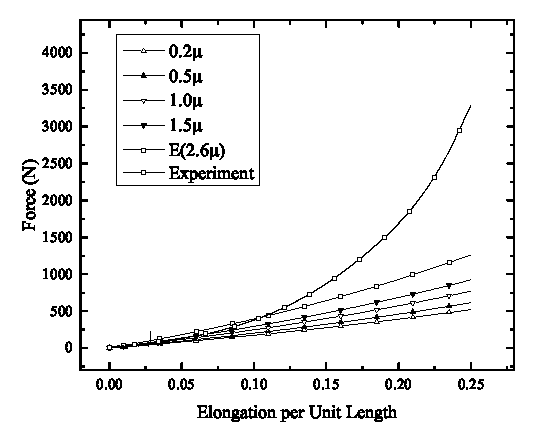
\includegraphics[width=0.45\linewidth]{figure/chap5/Various-Mu.eps}
	\label{fig:VariousMu}
	}
\subfigure[局部(应变$ 0\textasciitilde0.15 $)]{
	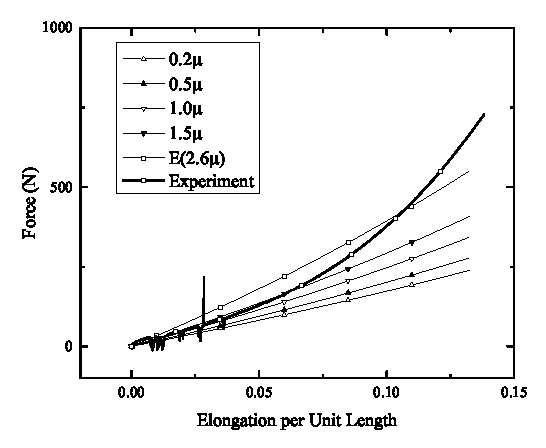
\includegraphics[width=0.45\linewidth]{figure/chap5/Various-Mu-small}
	\label{fig:Various-Mu-small}
	}
\fcaption{不同切向模量模型的力位移曲线}{load displacement  curves of models with various shear moduli}
\end{figure*}




由于编织相当紧密,假设两股纤维正交,单位宽度接触面可以提供相同宽度各向同性材料的切向刚度,根据几何关系,则有:

\begin{figure*}[!htb]
	\centering
	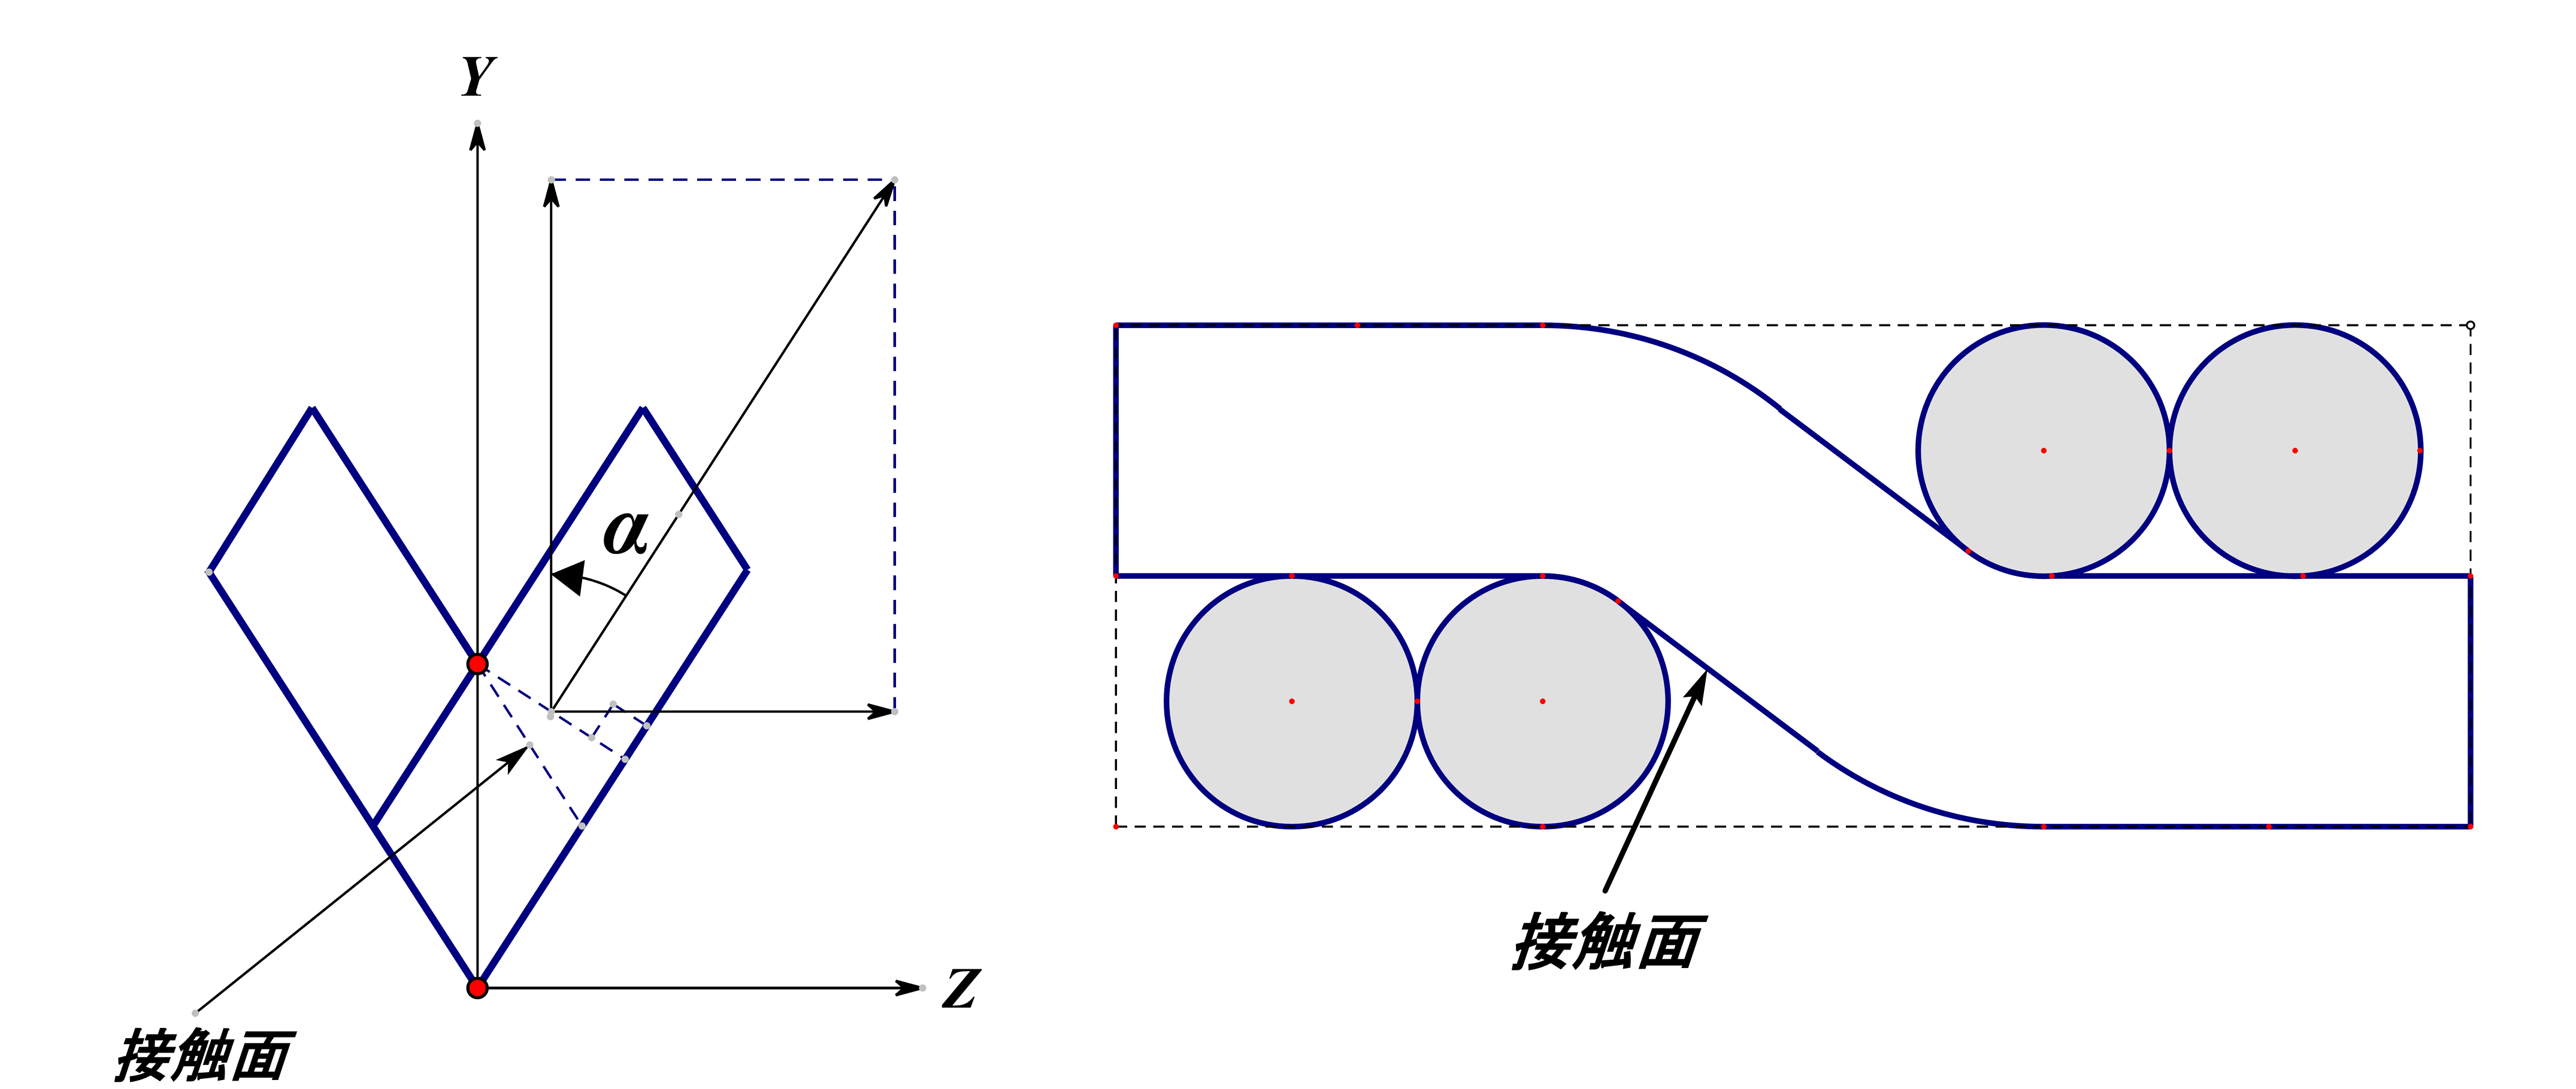
\includegraphics[height=0.25\textheight]{figure/chap5/modified-matrix}
	\fcaption{纤维间接触面几何关系}{geometry of the contact surface between fibers }
	\label{fig:modifiedmatrix}
\end{figure*}

\begin{equation}
\left\{ {\begin{array}{*{20}{c}}
{{C_{1212}} = \xi \mu  \cdot \sin \alpha }\\
{{C_{1313}} = \xi \mu  \cdot \cos \alpha }
\end{array}} \right.
\end{equation}








形成等效修正基体刚度矩阵为:
\begin{equation}
C_{ijkl}^{matrix} = \left[ {\begin{array}{*{20}{c}}
	{E\xi }&0&0&0&0&0\\
	0&0&0&0&0&0\\
	0&0&0&0&0&0\\
	0&0&0&{\mu \xi \cos \alpha }&0&0\\
	0&0&0&0&{\mu \xi \sin \alpha }&0\\
	0&0&0&0&0&0
	\end{array}} \right]
\end{equation}


编织层完整的刚度矩阵为:


\begin{equation}
C_{total}= {C_f} + C_{matrix}
\end{equation}


补充刚度矩阵后,才能进行完整的三维有限元分析。后续的有限计算结构默认补充$ C_{matrix} $。
但是模型仍然不能体现出拉伸试验中的非线性,需要在其他方向继续都模型进行修正。


\subsection{有限元试算结果}

有限元试算结果如\ref{fig:shisuan-1}所示。结合修正基体法后,基本没有表现出非线性行为。但从有限元仿真的角度来说,这是一个必要的过程,因为要进行更贴近实际工况的仿真,必须采用三维单元。补充修正刚度之后,刚度矩阵才满足$ 6\times6 $,可以进行三维有限元分析。
\begin{figure*}[!htp]
\centering
\subfigure{
	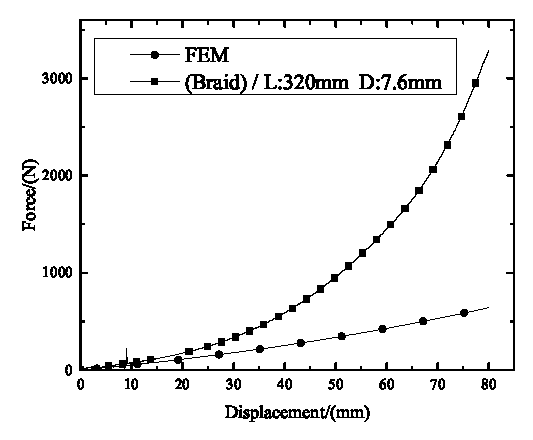
\includegraphics[width=0.45\linewidth]{figure/chap5/Ex-1-Origin}
	\label{fig:Ex-1-Origin}
	}
\subfigure{
	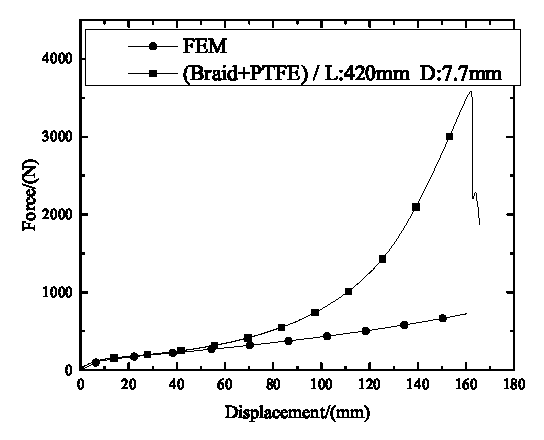
\includegraphics[width=0.45\linewidth]{figure/chap5/Ex-2-Origin}
	\label{fig:Ex-2-Origin}
	}
\fcaption{经过"修正基体法"修正的模型力位移曲线}{load displacement curve of the models modified by "modified matrix method"}
\label{fig:shisuan-1}
\end{figure*}



\section{编织角加速系数}


对比有限元模型与实验测得的编织角的变化,实验中编织角变化的速度更快(如图 \ref{fig:Graph30}所示),因此需要修正编织角理论,加速编织角的变化。
 
 \begin{figure*}[!htp]
\centering
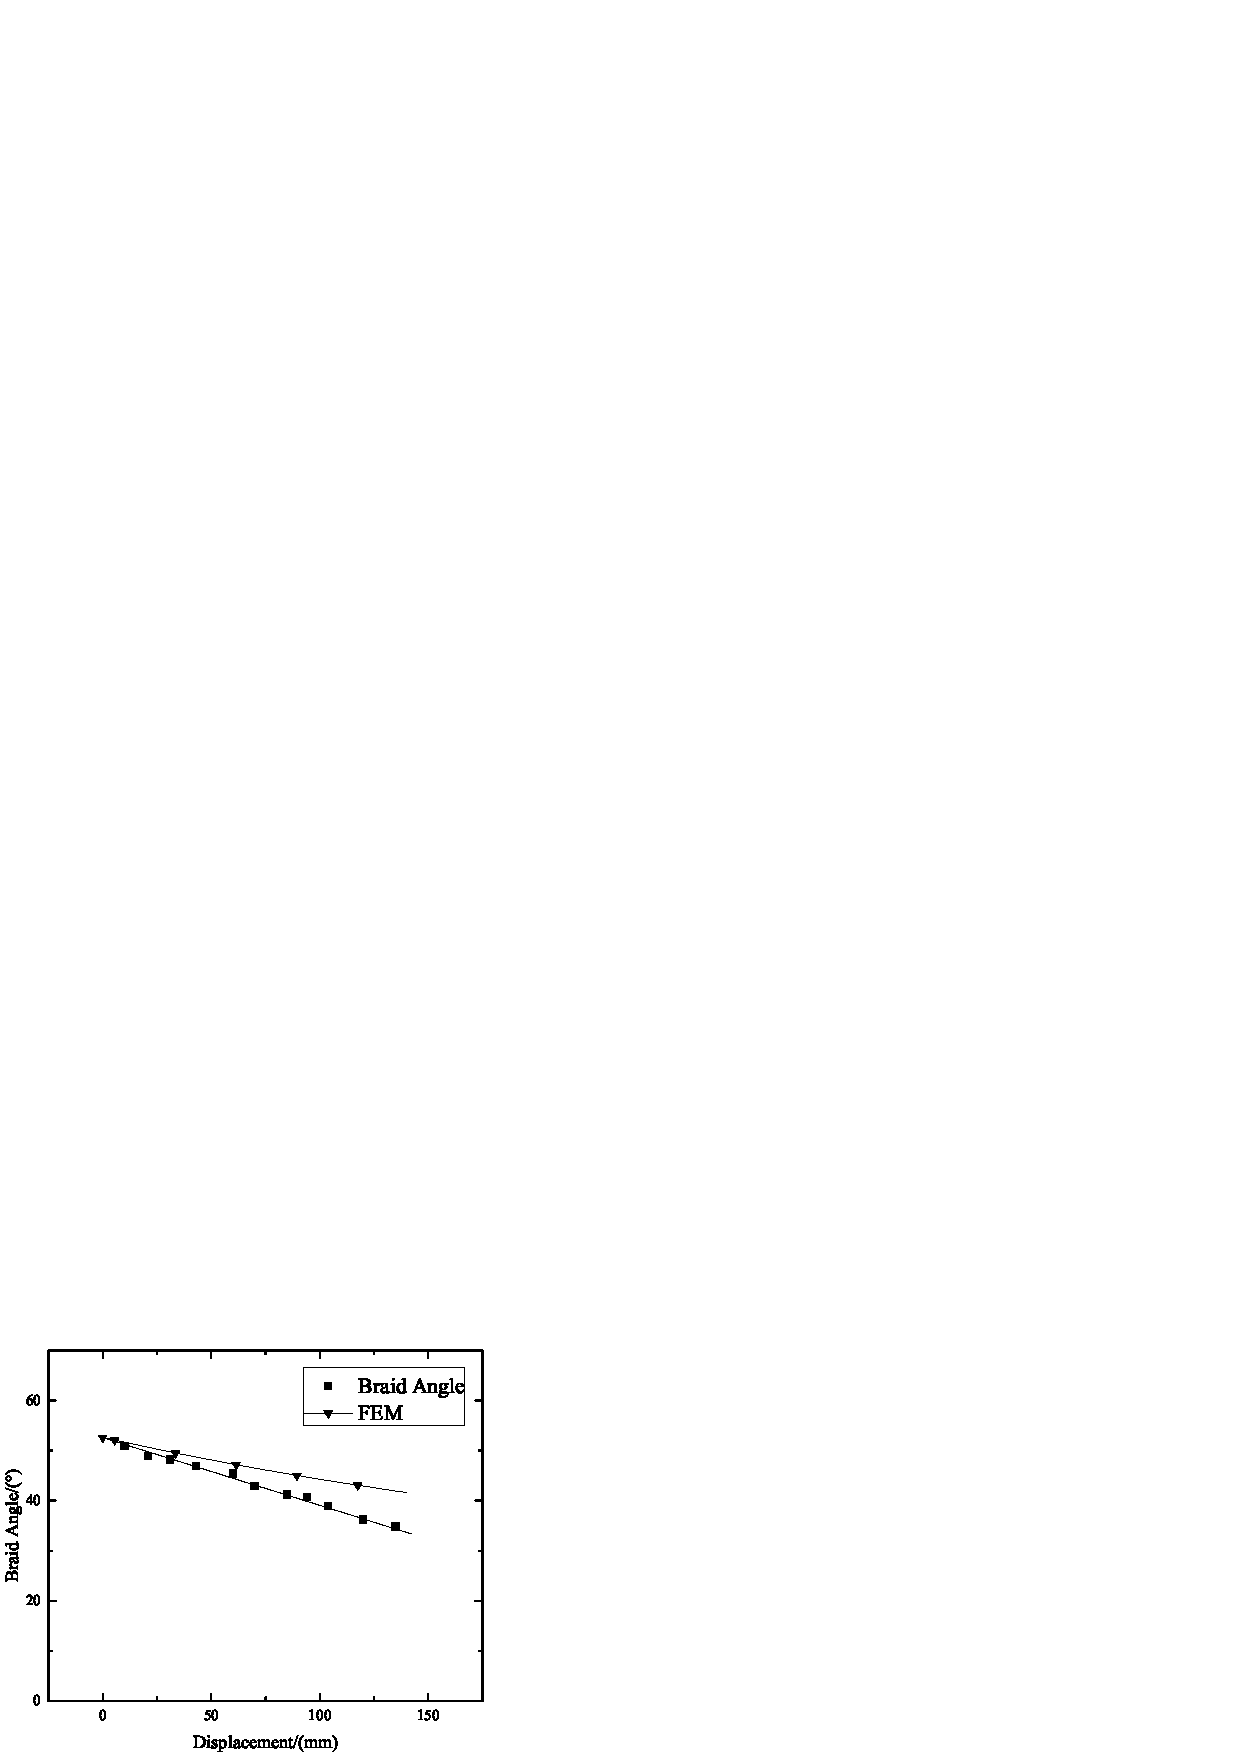
\includegraphics[width=0.5\linewidth]{figure/chap5/Graph30}
\fcaption{编织角变化实验结果对比有限元仿真结果(编织角-位移曲线)}{contrast of experimental and FEM results in braid angle change}[有限元编织角变化对比]
\label{fig:Graph30}
\end{figure*}

这种接触没有包含在等效修正基体中。金属纤维发生角度变化的过程中,各股金属纤维之间的侧向接触关系较为复杂,同时偶合了纤维本身的弯曲、扭转、摩擦等复杂情况。
这里提出一个简化假设:假设这些复杂的传力机制在编织层轴向上产生的效果,假设可以简化为特征单元轴向上的一组性弹簧,如图 \ref{fig:k-2}。 $ \alpha $ 可以该理解为特征单元中传力路径的方向,可以通过使得特征单元受力平衡的外力的偏离轴向的角度来表征。由于轴向弹簧、金属纤维的伸长,最终会合成一个偏离金属纤维的合力,则如图\ref{fig:k-3}所示,特征单元平衡时外力将会有 的额外转角。
\begin{figure*}[!htp]
\centering
	\hspace{0.5cm}
\subfigure[]{
	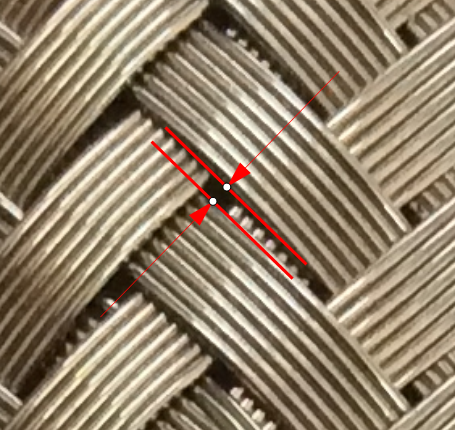
\includegraphics[height=0.12\textheight]{figure/chap5/k/1}
	\label{fig:k-1}
	}
	\hspace{0.5cm}
\subfigure[]{
	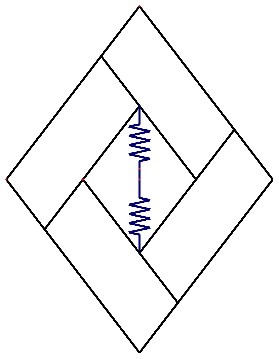
\includegraphics[height=0.13\textheight]{figure/chap5/k/2}
	\label{fig:k-2}
}
	\hspace{0.5cm}
\subfigure[]{
	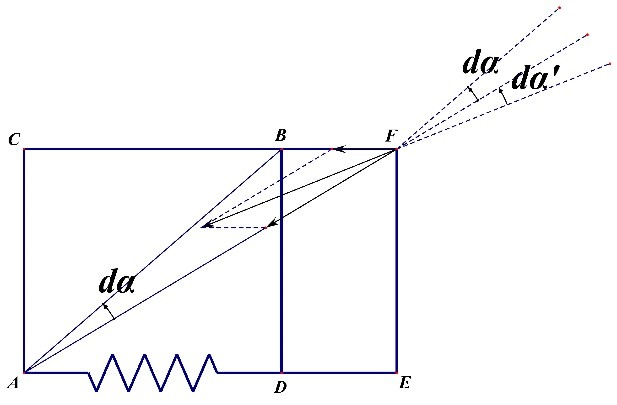
\includegraphics[height=0.15\textheight]{figure/chap5/k/3}
	\label{fig:k-3}
}
\fcaption{加速系数的模型}{model of braid angle coefficient }
\end{figure*}



这就需要编织角理论能够反映这种额外的转角。在(8)式中引入加速编织角变化的经验修正函数 $ \Phi \left( {\alpha ,D} \right) $,$ \alpha  $ 、$ D $ 分别为编织角与直径,表示该函数可能与软管的几何参数相关。
	  
	  

\begin{equation}
d\alpha  = \Phi \left( {\alpha ,D} \right) \cdot \frac{{{\varepsilon _{22}}\sin \alpha \cos \alpha }}{{1 + {\varepsilon _{22}}{{\cos }^2}\alpha }}
\end{equation}


根据实验结果及提出的假设:编织角变化在加载速度恒定的位移荷载下呈线性变化。因此,经验修正函数可能仅包含常数项:


\begin{equation}
\Phi \left( {\alpha , D} \right) = k
\end{equation}


\subsection{有限元试算结果}

$ k $ 值由不同的编织结构确定。按照修正编织角理论,有限元计算结果如图 \ref{fig:k-results}所示: 

\begin{figure*}[!htp]
\centering
\subfigure[$ k=3.0 $( 试算试件-1)]{
	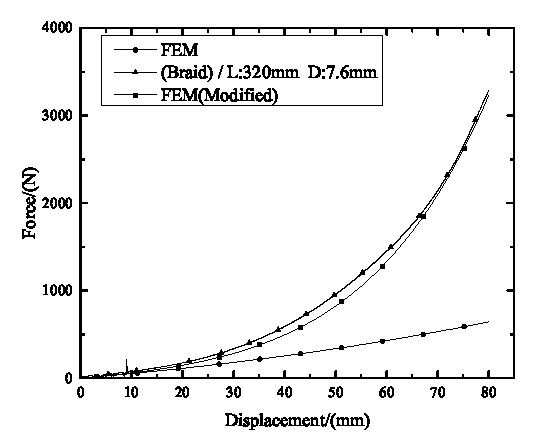
\includegraphics[height=0.2\textheight]{figure/chap5/Ex-1-Com}
	\label{fig:k-Ex-1-Com}
	}
\subfigure[$ k=2.3 $ ( 试算试件-2)]{
	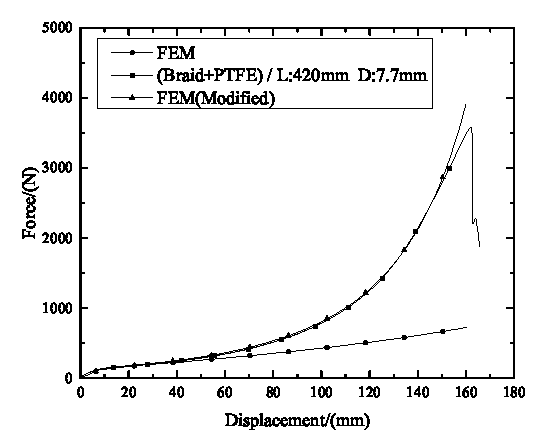
\includegraphics[height=0.2\textheight]{figure/chap5/Ex-2-Com}
	\label{fig:k-Ex-2-Com}
}
\subfigure[实验3-1-BD90]{
	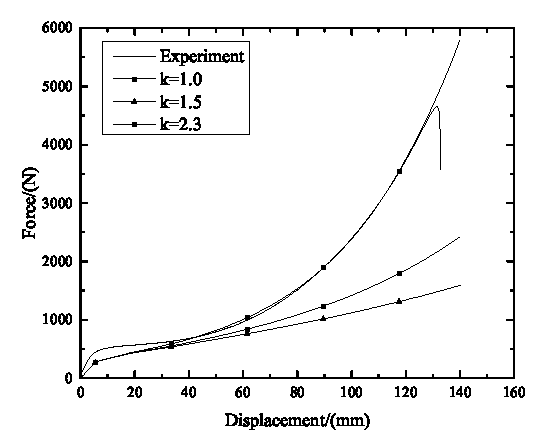
\includegraphics[height=0.2\textheight]{figure/chap5/Graph29}
	\label{fig:k-Graph28}
}
\subfigure[有限元编织角变化与实验对比]{
	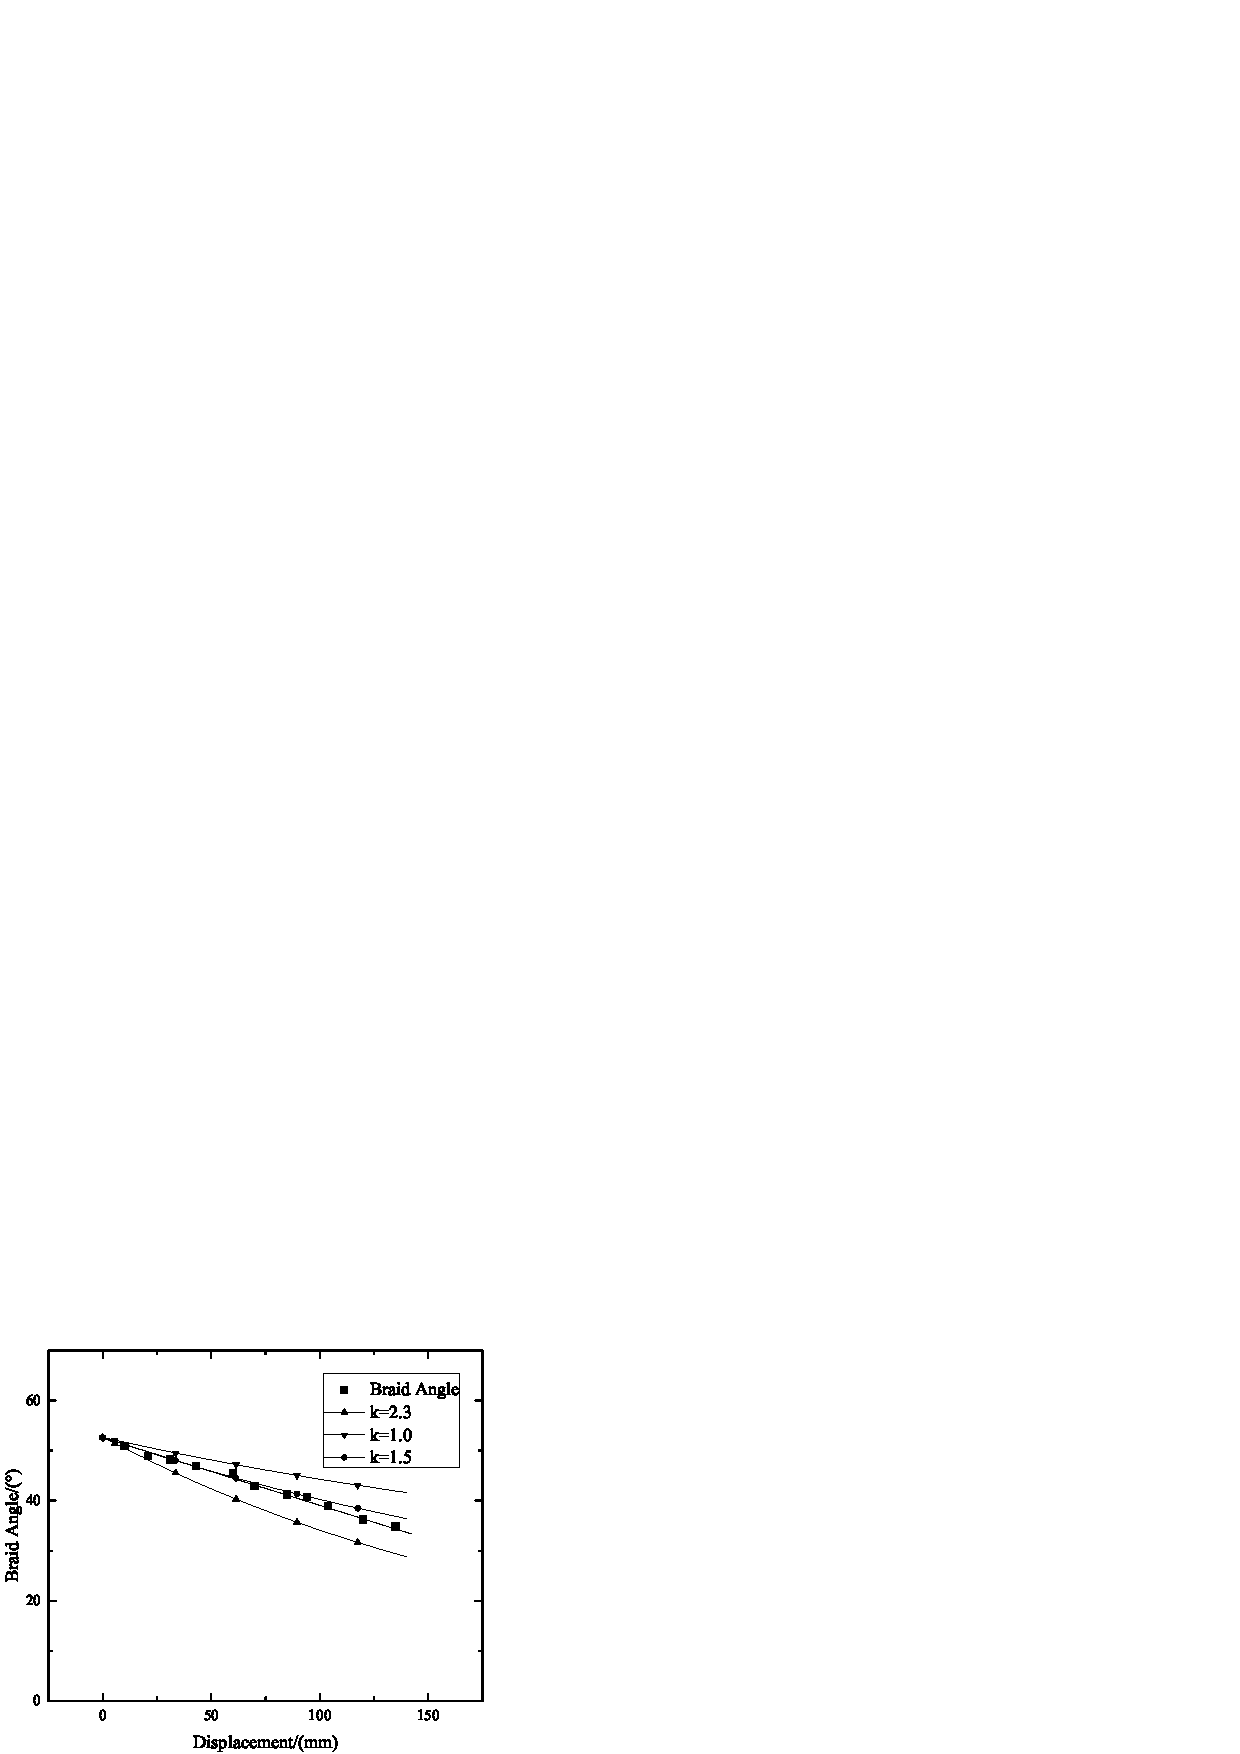
\includegraphics[height=0.2\textheight]{figure/chap5/Graph28}
	\label{fig:k-Graph29}
}
\fcaption{加速系数$ k $修正后的有限元仿真结果}{FEM results of models modifed by braid angle coefficient }
\label{fig:k-results}
\end{figure*}






图 \ref{fig:k-Graph28}、\ref{fig:k-Graph29}中,分别为$ k $取不同值时,软管模型力-位移曲线、编织角变化曲线。可以发现,当
$ k=2.3 $时,有限元模型的力-位移曲线与实验基本吻合,但编织角的变化的趋势要大于实验;当$ k=1.5 $时,有限元模型的编织角变化趋势与实验相近,但力-位移曲线趋势与实验相差较大。这意味着当编织角确定时,修正后的单元刚度仍小于实际情况;也可以认为,本模型可以表征金属编织软管的拉伸受力情况,但编织角偏转的理论值要大于实际值,有限元模拟中$ \alpha $ 超过实际编织角的部分就是由这部分额外的转角导致的。因此,加速系数k实际上有着很大的物理意义,它实际上涵盖了金属纤维间侧向接触,以及纤维间摩擦的作用效果。


尽管这种接触可以等效为弹簧,但是确定弹簧的弹性系数比较困难,因为这个系数很有可能是非线性的:单股纤维转动时,首先填满各股之间空隙,此时轴向弹性较小;随着拉伸荷载增大,纤维自身弯曲扭转,纤维间压紧,摩擦增大,轴向弹性效果可能会明显增强。要量化确定这个过程,需要进一步实验的支持。



\section{编织角理论修正}
\ha 的理论中,编织层管径的变化采用钢绞线理论,如式\ref{eq:d-chap5}、\ref{eq:l-chap5}所示。但是这样的处理方法并不能准确的反应管径的变化,从结果上来时导致了整体非线性不足

\begin{equation}
\label{eq:d-chap5}
D = {D_0}\frac{{\sin \left( \alpha  \right)}}{{\sin \left( {{\alpha _0}} \right)}}
\end{equation}

\begin{equation}
\label{eq:l-chap5}
L = {L_0}\frac{{\cos \left( \alpha  \right)}}{{\cos \left( {{\alpha _0}} \right)}}
\end{equation}




而软管组件的内管刚度较低容易被压缩;受内压荷载的状态下,管径的变化也是一个很重要的因素,因此管径的变化应该直接在特征单元中体现。图\ref{fig:unit-cell-3}为特征单元考虑管径的修正方案。根据几何关系可得:

\begin{figure*}[!htb]
\centering
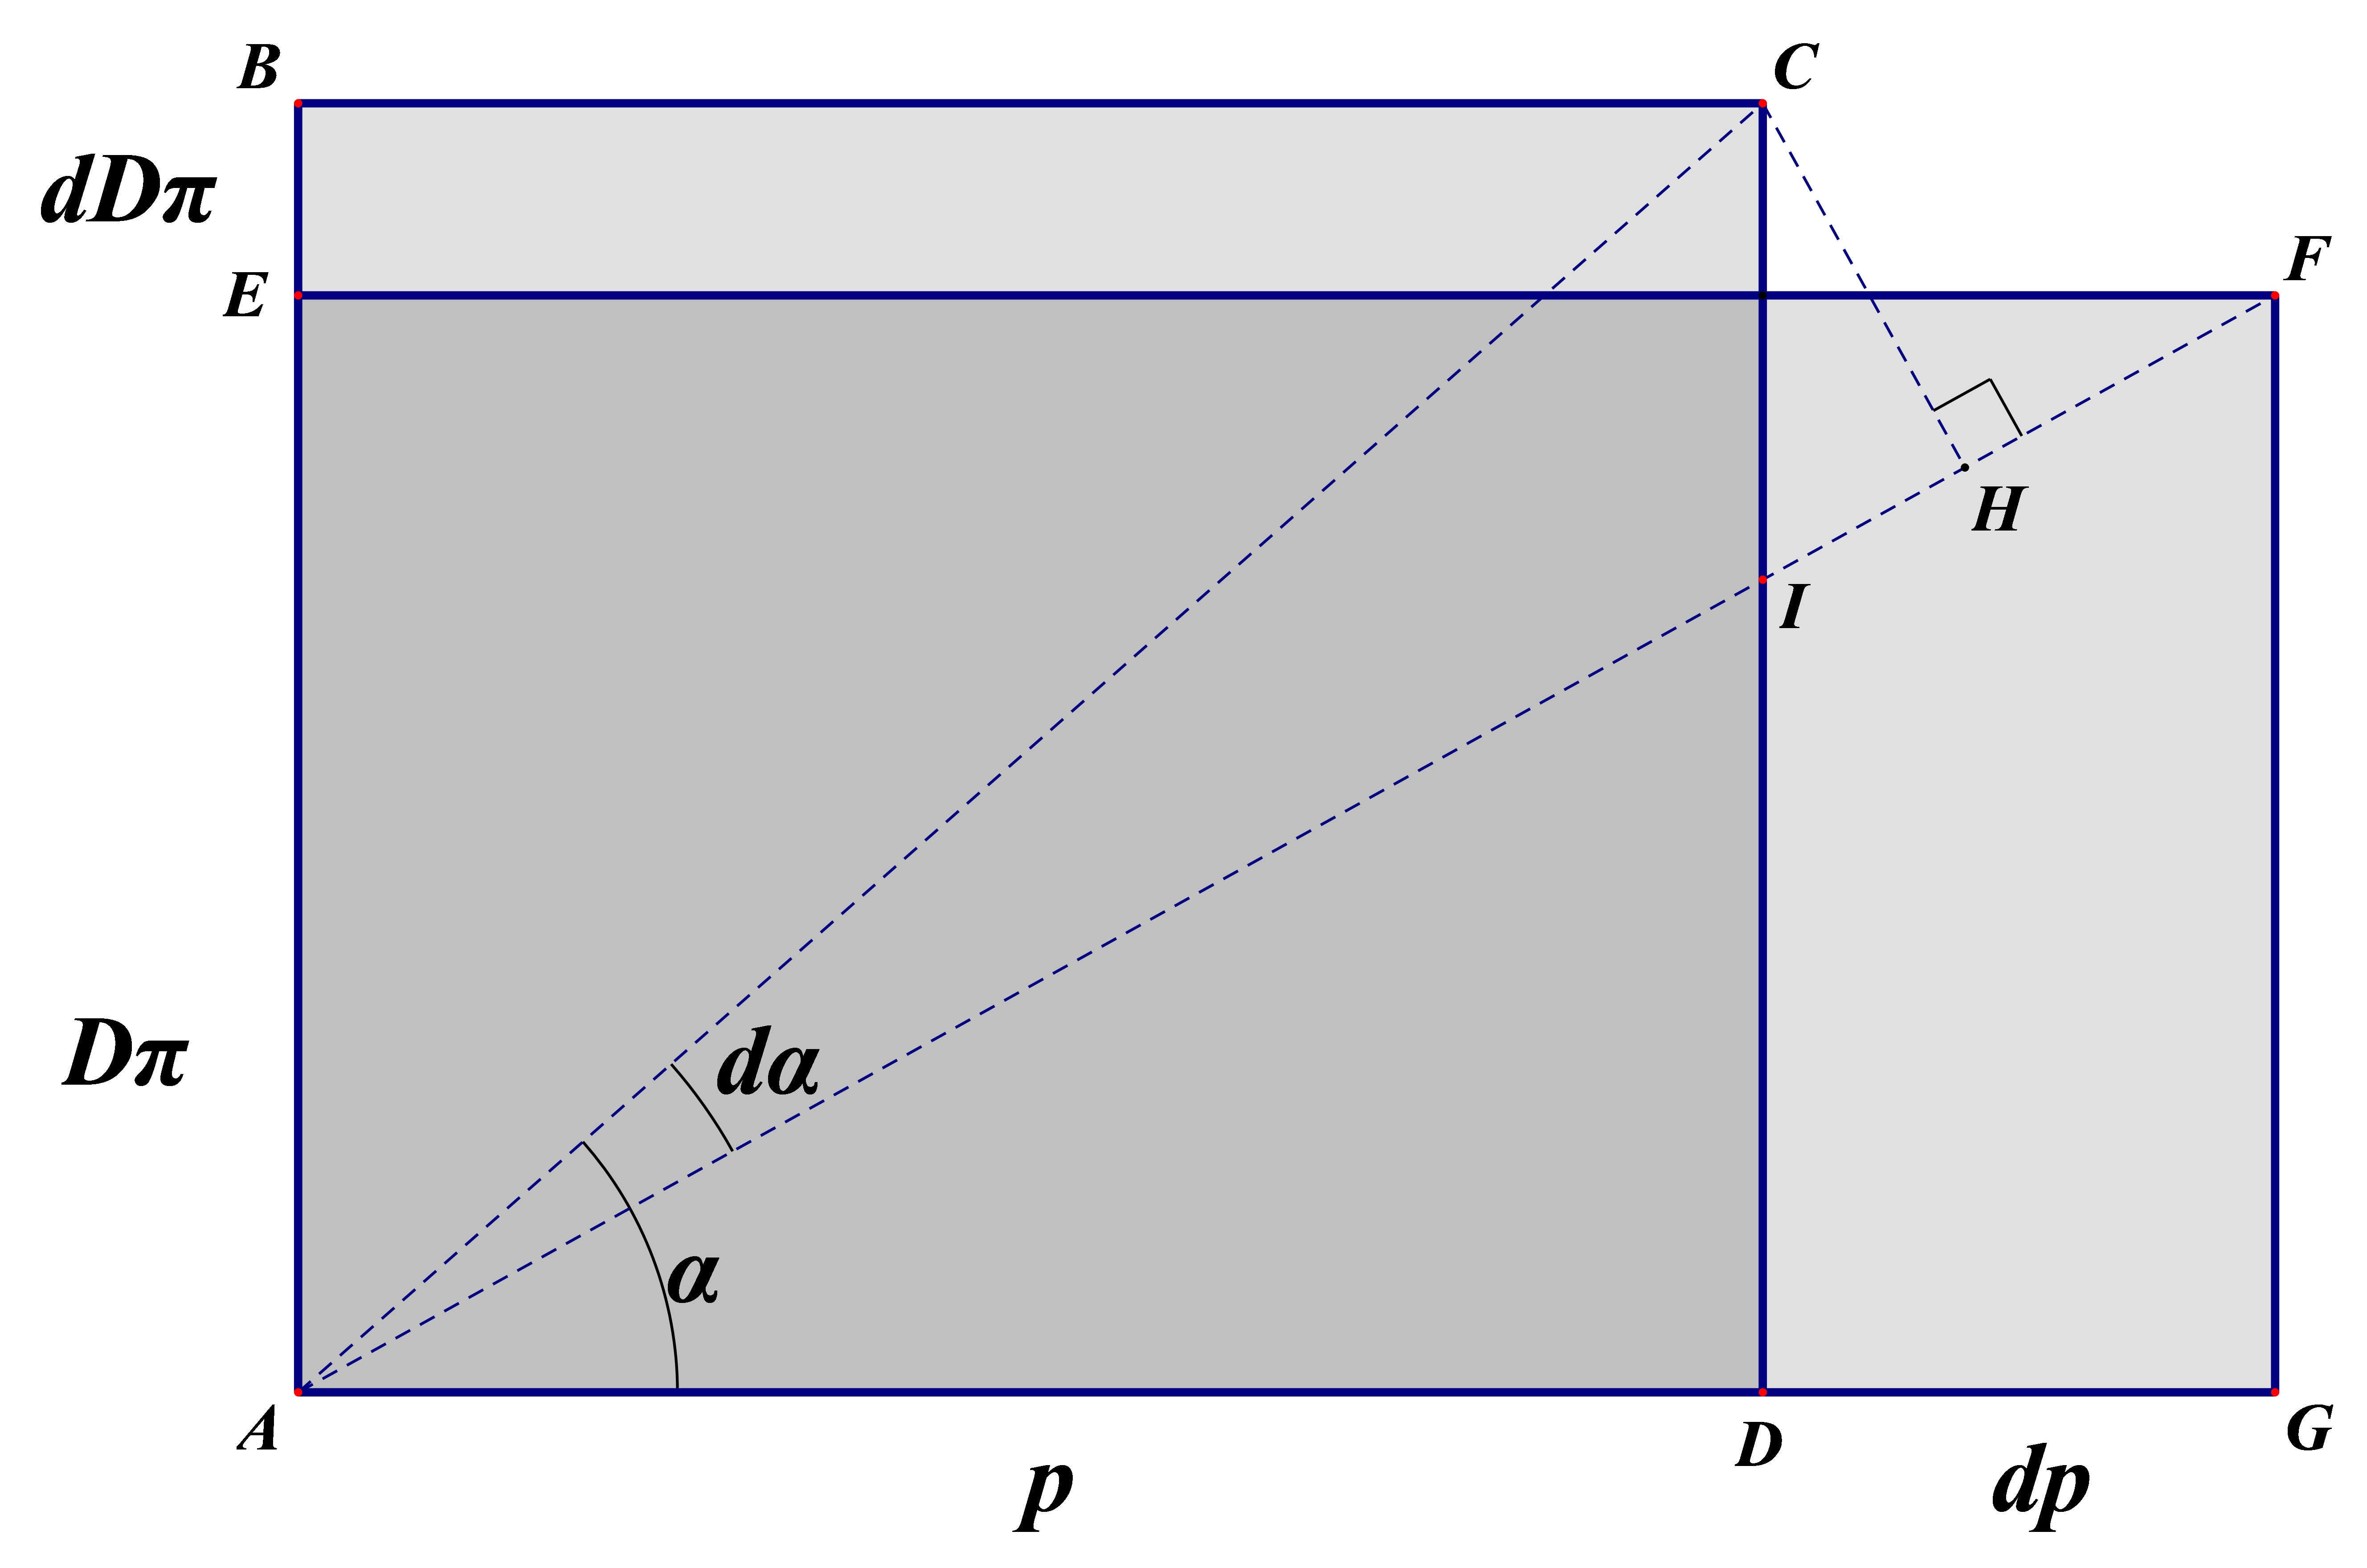
\includegraphics[height=0.2\textheight]{figure/chap5/unit-cell-3}
\fcaption{特征单元的编织角变化几何关系修正}{modified geometry of braid angle change}
\label{fig:unit-cell-3}
\end{figure*}

纤维的伸长量为:

\begin{equation}
\begin{array}{*{20}{c}}
{{\varepsilon _{33}} = \frac{{dD}}{D}}&{{\varepsilon _{22}} = \frac{{dP}}{P}}
\end{array}
\end{equation}

\begin{equation}
d\alpha  = \frac{{\left( {{\varepsilon _{22}} + {\varepsilon _{33}}} \right)\sin \left( \alpha  \right){\rm{cos}}\left( \alpha  \right)}}{{1 - {\varepsilon _{33}}{{\sin }^2}\left( \alpha  \right) + {\varepsilon _{22}}{\rm{co}}{{\rm{s}}^2}\left( \alpha  \right)}}
\end{equation}


\begin{equation}
{\varepsilon _f} = \sqrt {\frac{{{{\left( {{\varepsilon _{22}} + 1} \right)}^2} + \tan {\alpha ^2}{{\left( {1 - {\varepsilon _{33}}} \right)}^2}}}{{1 + \tan {\alpha ^2}}}}  - 1
\end{equation}


\subsection{有限元试算结果}
利用修正后的编织角理论进行有限元仿真试算,结果如图\ref{fig:RUC-MOD}所示,力位移曲线出现了明显的非线性。
\begin{figure*}[!htp]
\centering
\subfigure[实验试件-1]{
	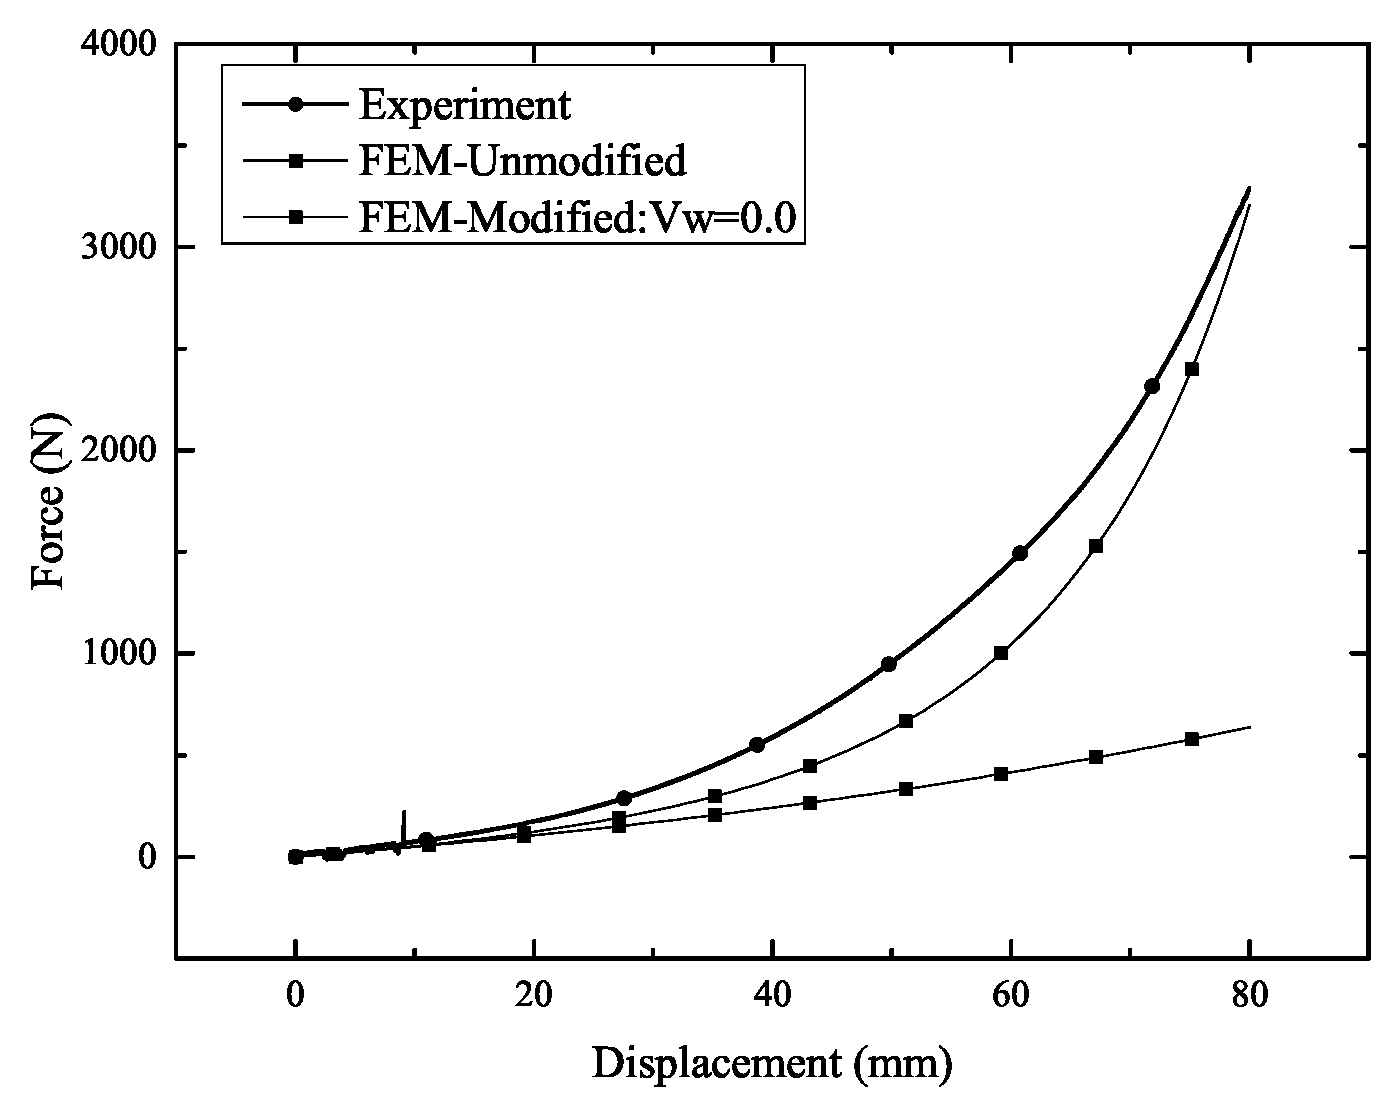
\includegraphics[width=0.45\linewidth]{figure/chap5/sp1/RUC-mod}
	}
\subfigure[实验试件-2]{
	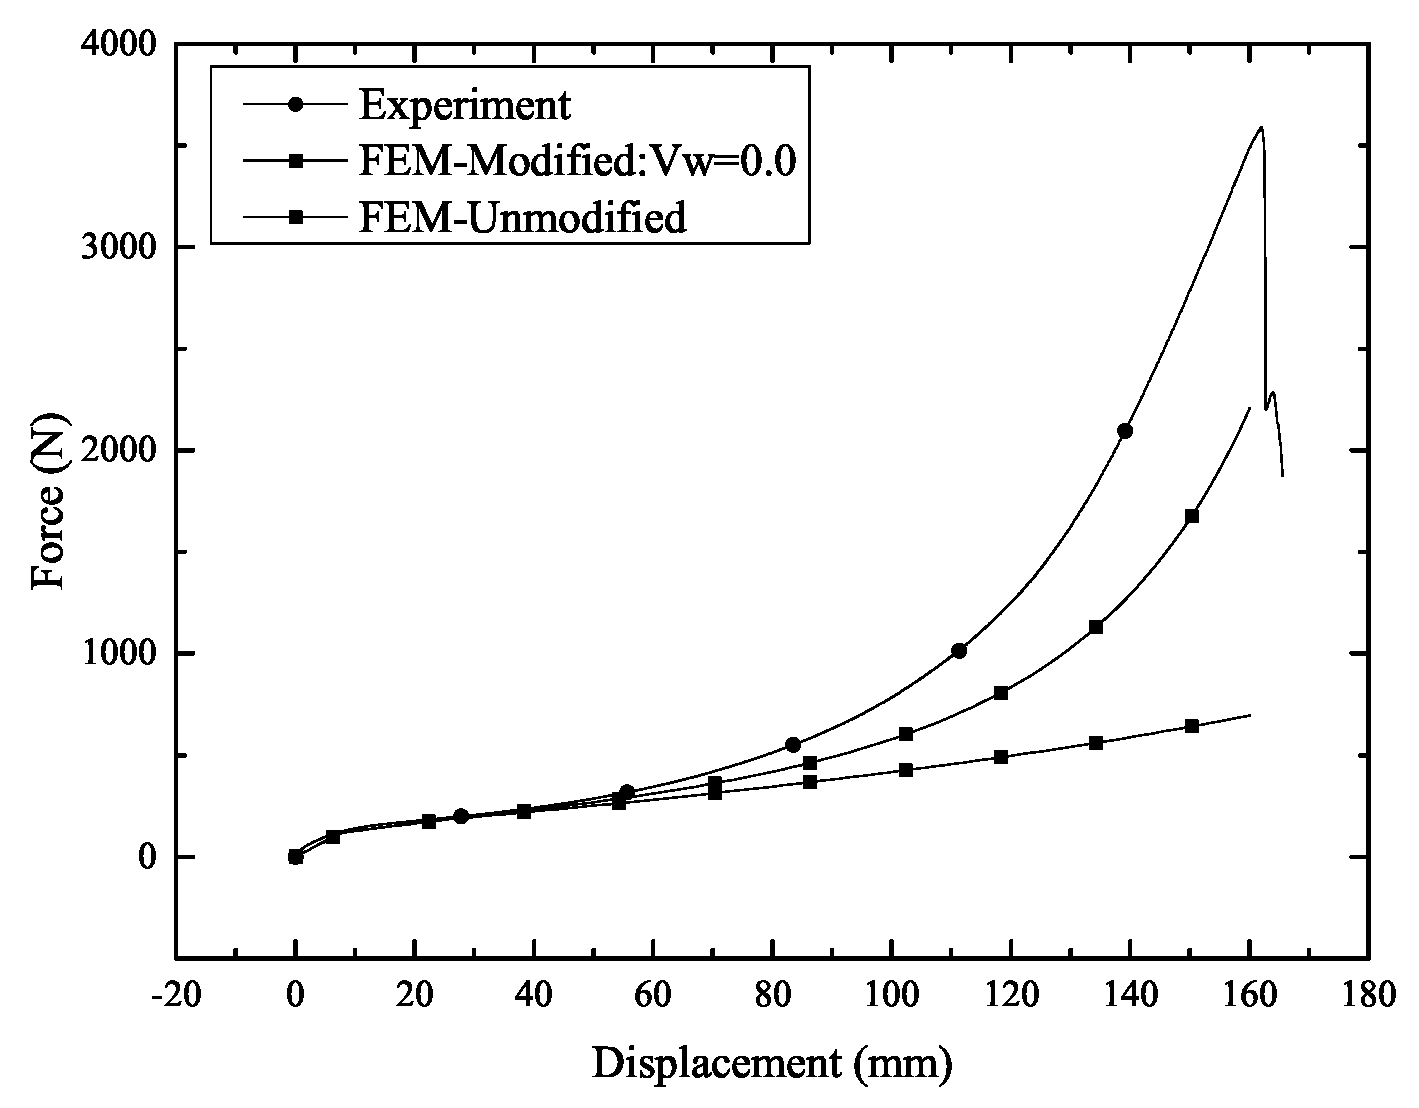
\includegraphics[width=0.45\linewidth]{figure/chap5/sp2/RUC-MOD}
	}
\fcaption{修正编织角理论有限元试算结果}{}
\label{fig:RUC-MOD}
\end{figure*}






\section{三维线型修正}

实际上,仅仅把纤维简化为平面2D的特征单元是不够的,实际如\ref{fig:3d-wire-3}所示,对于$ 2\times 2 $编织形式的非金属纤维编织层,至少$ 50 \% $的纤维处于斜穿状态。

\subsection{斜穿纤维角度的计算}
一般高密度编织层中,纤维相互紧贴,截面编织密度$ {\xi _{section}} \approx 1 $,根据式\ref{eq:section-epsilon}可得编织层厚度,也就是斜穿纤维厚度方向上传过的距离为:


\begin{equation}
\tau \phi  = D - \sqrt {{D^2} - \frac{{{N_S}{N_W}{\phi ^2}}}{{\cos \alpha }}} 
\end{equation}

如图\ref{fig:3d-wire-3}所示,斜穿的纤维,投影在编织平面内的头投影的长度为:
\begin{equation}
\frac{{{N_W}\phi }}{{\sin 2\alpha }}
\end{equation}
则斜穿纤维偏离平面的角度为
\begin{equation}
\frac{\pi }{2} - \varphi  = \arctan \frac{{\tau \phi}}{{{N_W}\phi }}
\end{equation}

以\shii 为例,将其参数代入可得纤维偏离平面的角度$ \frac{\pi }{2} - \varphi  $为$ 26.9\textdegree $。



\subsection{考虑斜穿纤维的刚度计算}

对于金属纤维的编织层,金属纤维由于刚度较高,会保持类似于正弦函数图像的线型。如图\ref{fig:sin-xianxing}所示。这也导致了一层金属编织层的厚度一般大于两层缠绕成。针对这种弯曲纤维,\citeauthor{russia1970}\cite{russia1970}提出了一种处理方法:

\begin{figure*}[!htb]
\centering
\subfigure[]{
	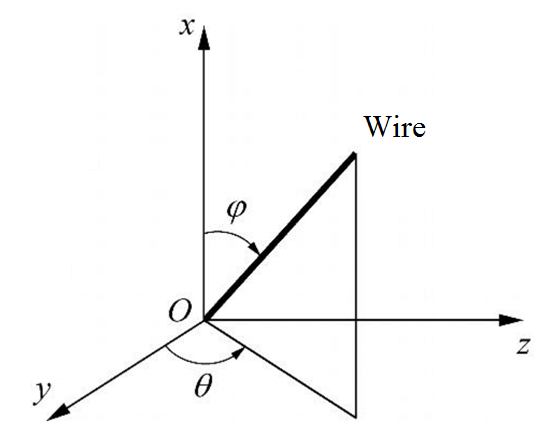
\includegraphics[height=0.2\textheight]{figure/chap5/3d-wire}
	}
\hspace{0.5cm}
\subfigure[]{
	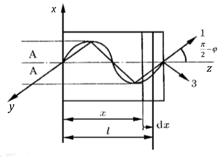
\includegraphics[height=0.2\textheight]{figure/chap5/3d-wire-2}
	\label{fig:sin-xianxing}
	}
\fcaption{编织层中斜穿的纤维}{}
\label{fig:3d-wire}
\end{figure*}






假设图	\ref{fig:sin-xianxing}中的纤维轨迹服从函数 $  f\left( x \right)$ 的规律,与平面的夹角$ \theta $可表示成:

\begin{equation}
\frac{\pi }{2} - \varphi   =  - \arccos \frac{1}{{\sqrt {1 + {{\left( {A\frac{{df\left( x \right)}}{{dx}}} \right)}^2}} }}
\end{equation}

结合修正基体法根据单向纤维复合材料微段$ dx $的柔度系数$ {{S_{ij}}^*\left( \frac{\pi }{2} - \varphi  \right)} $,通过曲线积分求得相应编织材料的有效性能为:

\begin{equation}
{S_{ij}} = \frac{1}{l}\int\limits_0^l {{S_{ij}}^*\left( \frac{\pi }{2} - \varphi \right)dx} 
\end{equation}

但这种处理方相对较为繁琐,本文选择较为类似的一种处理方法。$ 2\times 2 $编织形式可以近似看作图\ref{fig:3d-wire-3}中的形式,将编织层分为间隔交替的两种纤维分布形式。


\begin{figure*}[!htp]
	\centering
	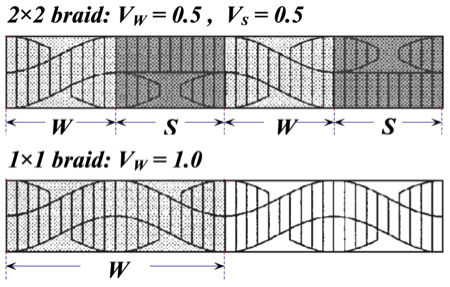
\includegraphics[height=0.2\textheight]{figure/chap5/3d-wire-3}
	\label{fig:3d-wire-3}
	\fcaption{不同编织形式中斜穿纤维的分布}{}
\end{figure*}

其中$ V_W $为斜穿纤维的体积比例;$ V_S $为平面内纤维的体积比例,纤维编织层整体的刚度矩阵为

\begin{equation}
{C_f} = {V_S} \cdot {C_{f,ijkl}}^S + {V_W} \cdot {C_{f,ijkl}}^W
\end{equation}

其中,$ {C_{f,ijkl}}^S $为平面内钢丝的刚度矩阵;为斜穿纤维部分的刚度矩阵,需要额外考虑纤维的取向,如图\ref{fig:3d-wire}所示,则有:

\begin{equation}
\left\{ \begin{array}{l}
{n_1} = \cos \varphi \\
{n_2} = sin\varphi \sin \theta \\
{n_3} = sin\varphi \cos \theta 
\end{array} \right.
\end{equation}

那么斜穿部分纤维的刚度矩阵$ {C_{f,ijkl}}^W $为:

\begin{equation}\small
E\xi  \cdot \left[ {\tiny \begin{array}{*{20}{c}}
{{{\cos }^4}\varphi }&{{{\cos }^2}\varphi {{\cos }^2}\theta }&{{{\cos }^2}\varphi {{\sin }^2}\theta }&{{{\cos }^3}\varphi \cos \theta }&0&0\\
{{{\cos }^2}\varphi {{\cos }^2}}&{{{\cos }^4}\theta }&{{{\cos }^2}\theta {{\sin }^2}\theta }&{\cos \varphi {{\cos }^3}\theta }&0&0\\
{{{\cos }^2}\varphi {{\sin }^2}\theta }&{{{\cos }^2}\theta {{\sin }^2}\theta }&{{{\sin }^4}\theta }&{\cos \varphi \cos \theta {{\sin }^2}\theta }&0&0\\
{{{\cos }^3}\varphi \cos \theta }&{\cos \varphi {{\cos }^3}\theta }&{\cos \varphi \cos \theta {{\sin }^2}\theta }&{{{\cos }^2}\varphi {{\cos }^2}\theta }&0&0\\
0&0&0&0&{{{\cos }^2}\varphi {{\sin }^2}\theta }&{\cos \varphi \cos \theta {{\sin }^2}\theta }\\
0&0&0&0&{\cos \varphi \cos \theta {{\sin }^2}\theta }&{{{\cos }^2}\theta {{\sin }^2}\theta }
\end{array}} \right]
\end{equation}

\subsection{斜穿纤维角度的影响}

斜穿纤维偏离编织层平面的角度为$ \frac{\pi }{2} - \varphi  $,图\ref{fig:phi-MOD}中分别为$ \frac{\pi }{2} - \varphi  = 0\textdegree/20\textdegree/40\textdegree/60\textdegree$的力位移曲线。该角度减小时,编织层整体在拉伸的过程中会体现更强的非线性,整体的刚度也会加强。
\begin{figure*}[!htp]
	\centering
	\subfigure[试验试件-1]{
		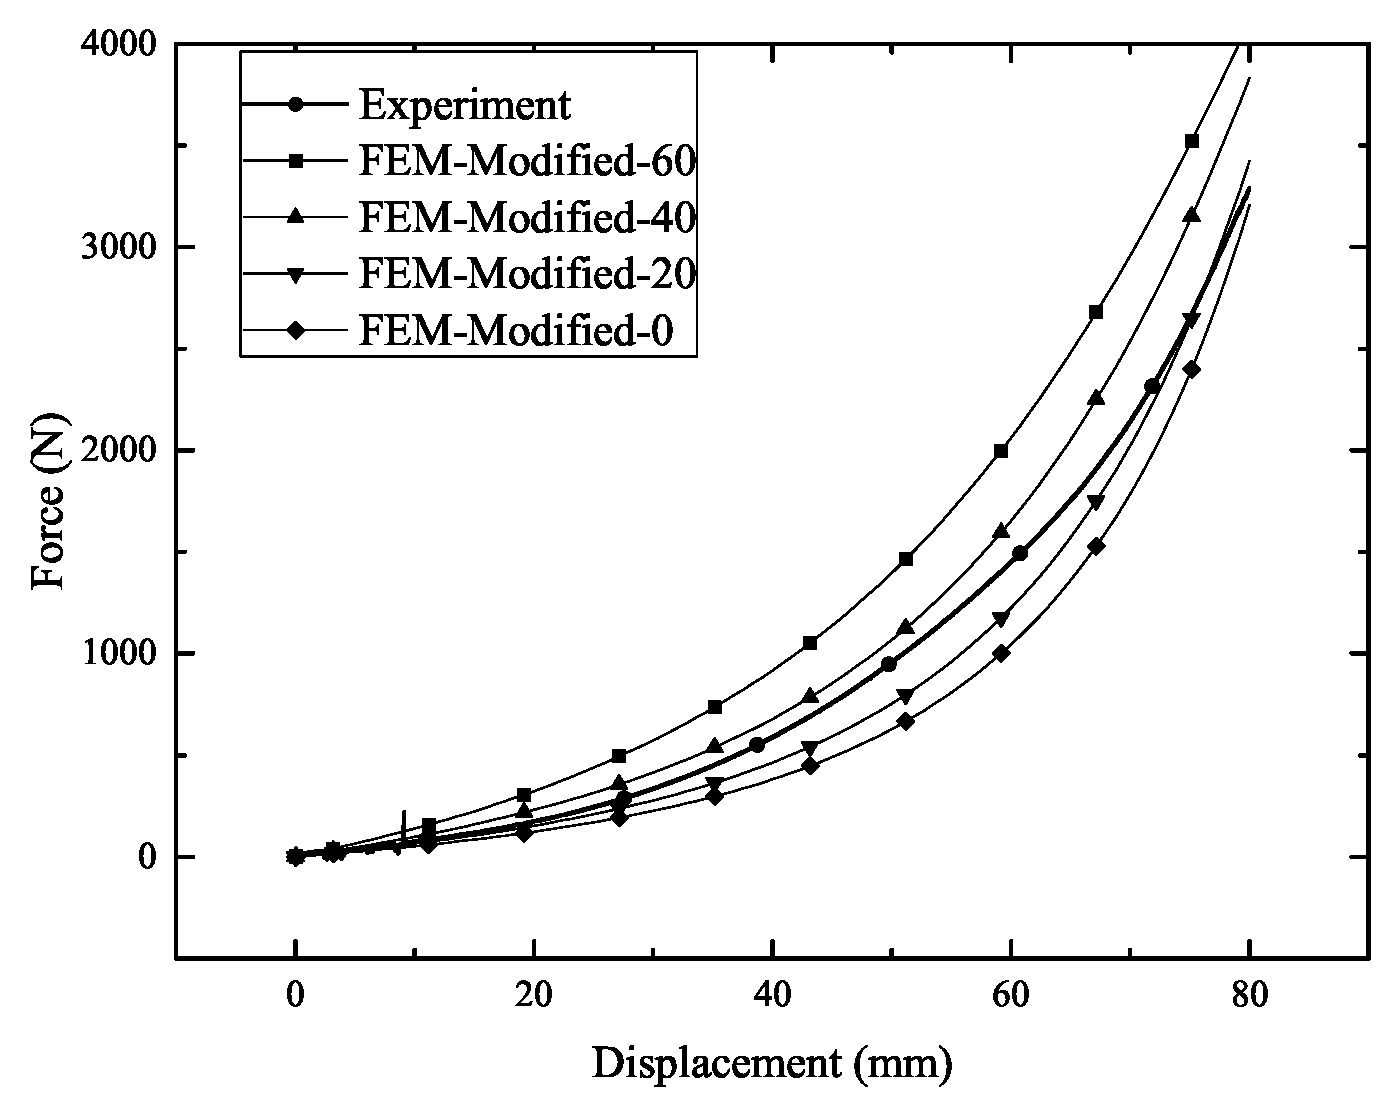
\includegraphics[height=0.35\textheight]{figure/chap5/sp1/phi-mod}
		}
		
	\subfigure[试验试件-2]{
		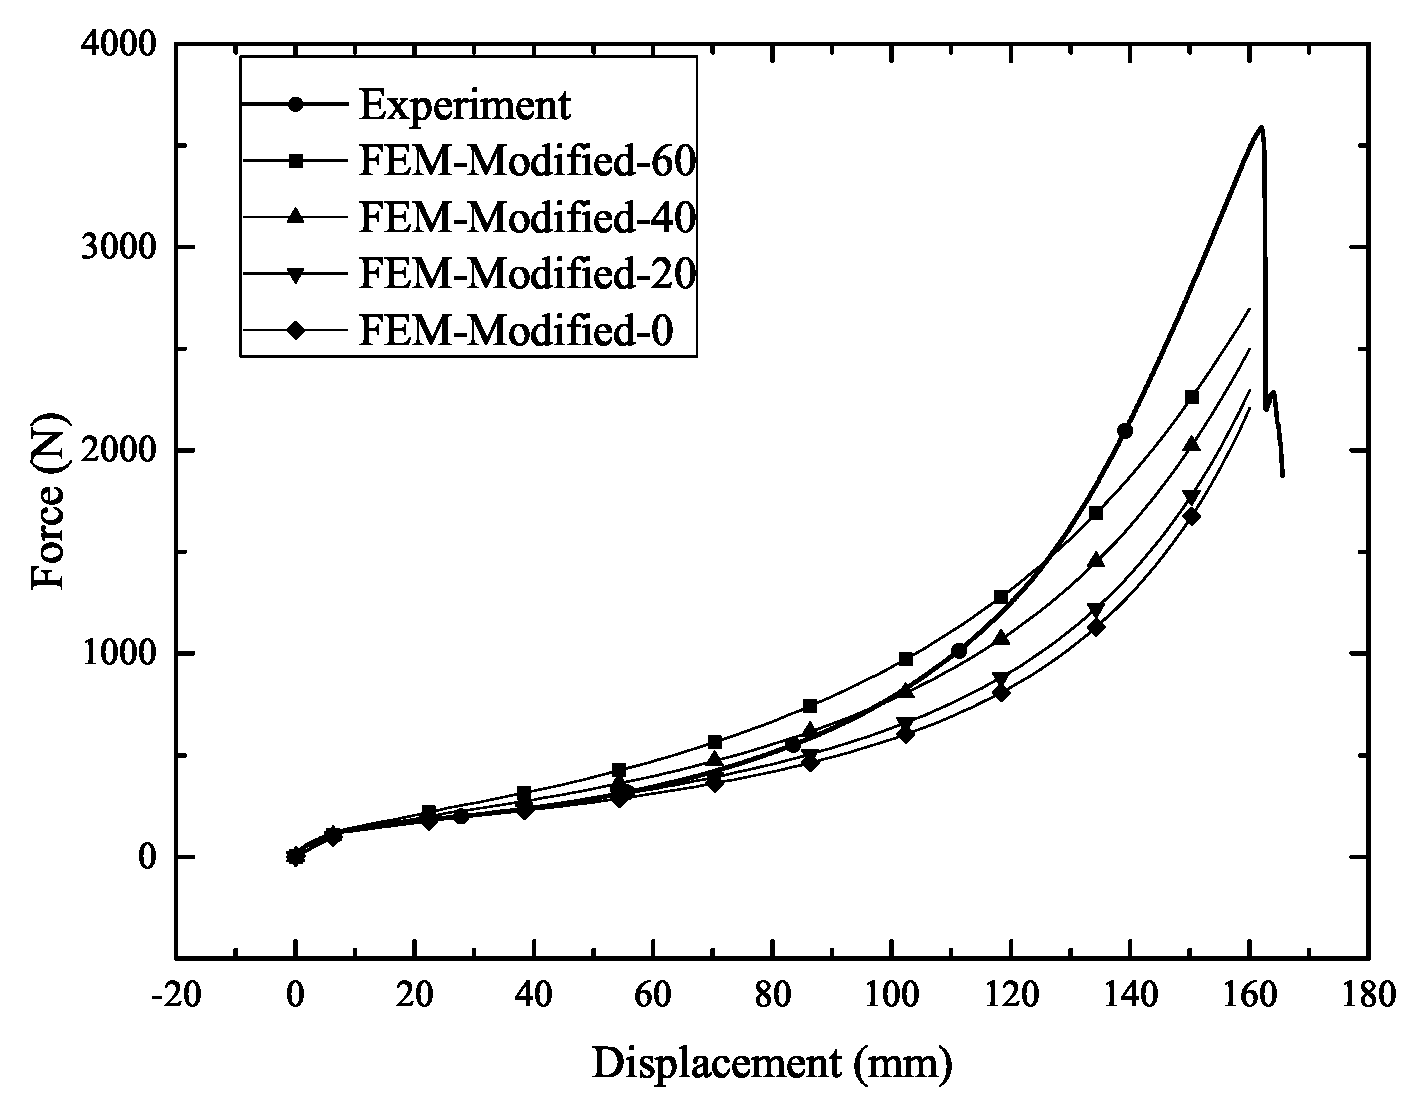
\includegraphics[height=0.35\textheight]{figure/chap5/sp2/phi-MOD}
		}
	\fcaption{纤维偏离角度的影响}{}
	\label{fig:phi-MOD}
\end{figure*}






\subsection{斜穿纤维体积比例对总体刚度的影响}

对于金属编织层,并不像复合材料编织层可以明确,因为金属纤维刚度较大,倾向于保持斜穿的状态。图\ref{fig:Vw-MOD}中为假设斜穿纤维体积分数从0到1的4中情况,$ V_W $为$ 0 $时,所有纤维都在编织层平面内。$ V_W=1.0  $时,所有纤维都是斜穿纤维。如图\ref{fig:Vw-MOD}中所示,斜穿纤维体积比例对总体刚度的影响不如纤维偏离角度的影响大。


\begin{figure*}[!htp]
\centering
\subfigure[实验试件-1]{
	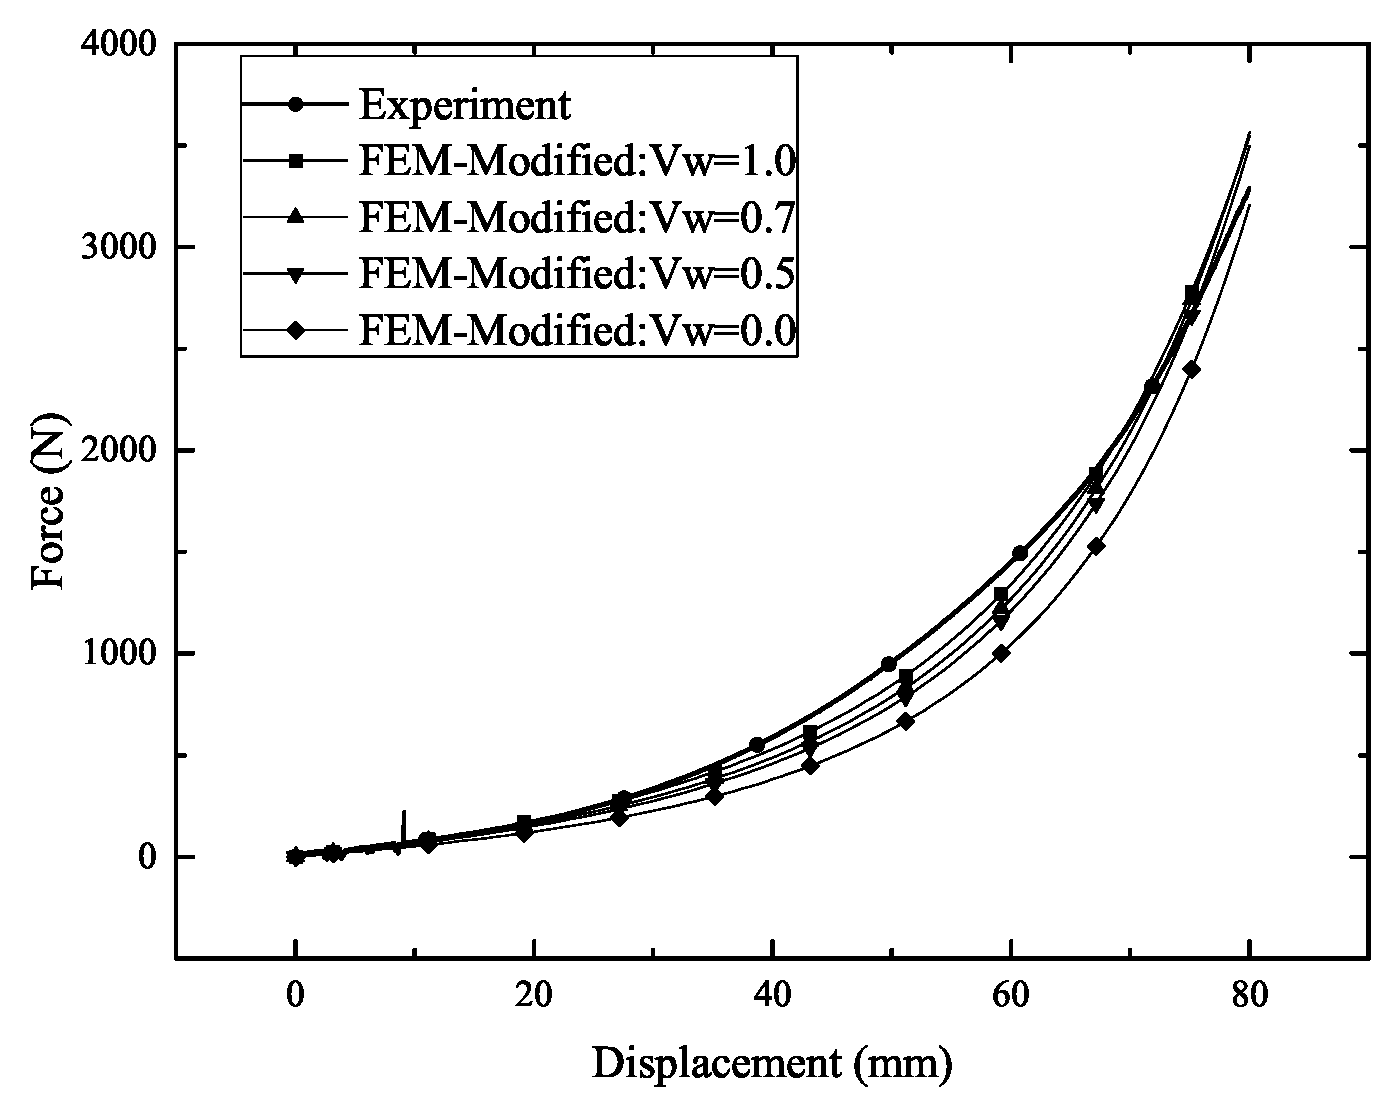
\includegraphics[width=0.6\linewidth]{figure/chap5/sp1/Vw-mod}
	}
\subfigure[实验试件-2]{
	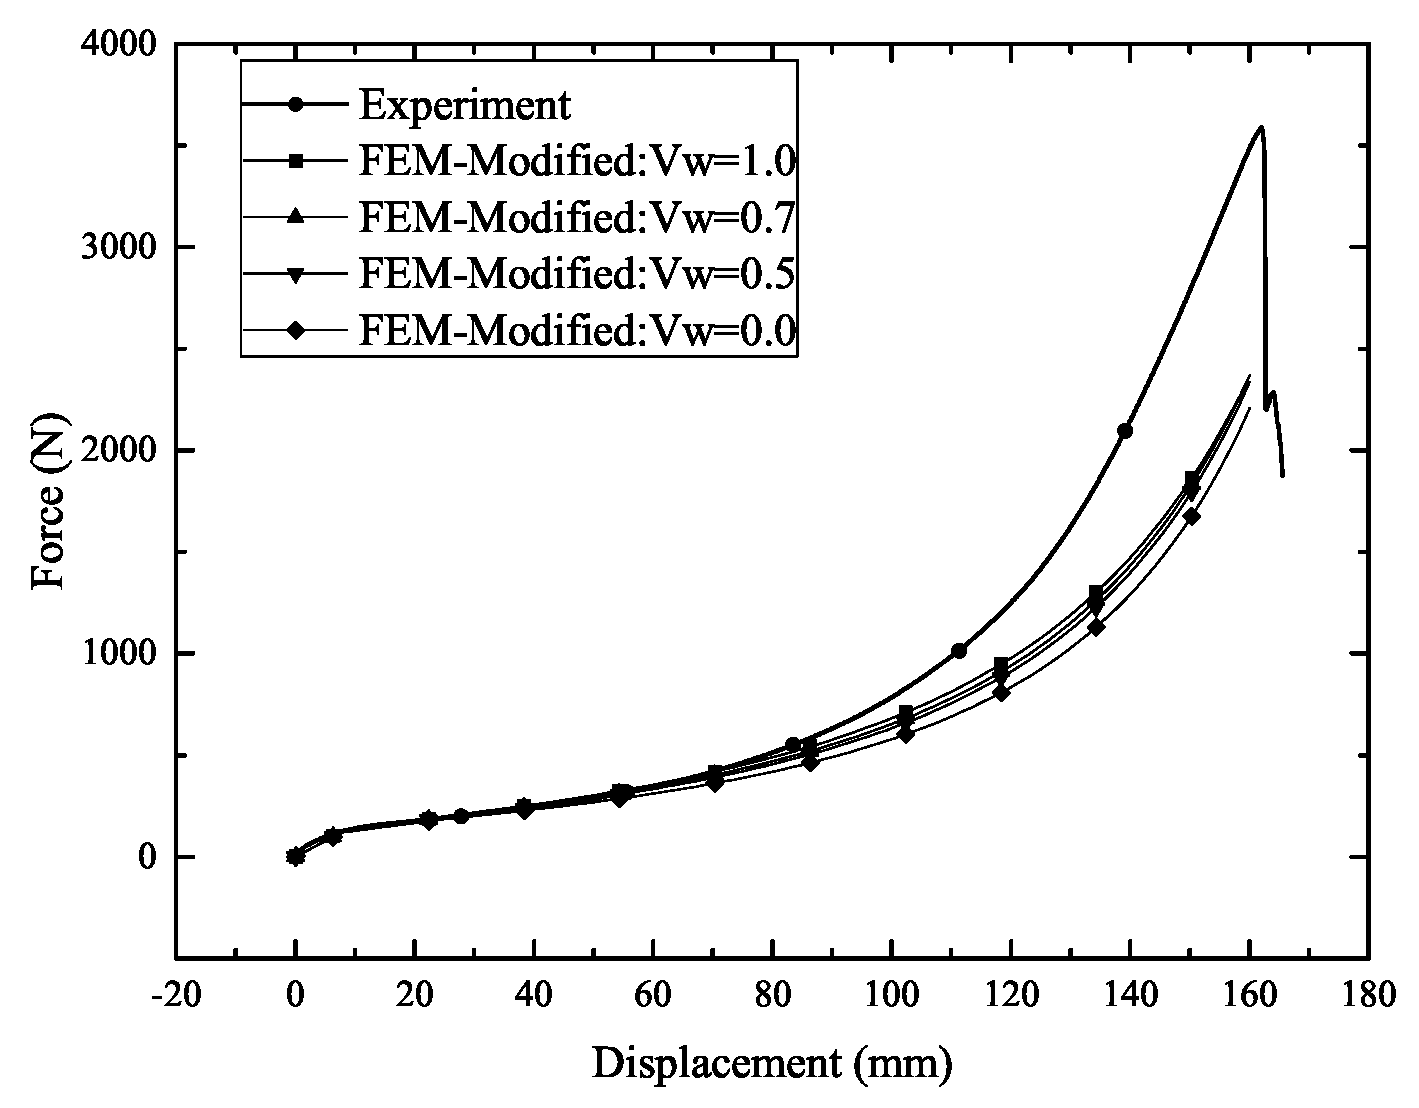
\includegraphics[width=0.6\linewidth]{figure/chap5/sp2/Vw-MOD}
	}
\fcaption{斜穿纤维体积比例对总体刚度的影响}{}
\label{fig:Vw-MOD}
\end{figure*}






\section{综合修正结果}

考虑以上所有的影响因素的编织层结构非线性行为的影响后,仿真结果的力位移曲线与实验结果仍有一定差距,这部分的差距可以通过编织角加速系数进行修正。如图\ref{fig:k-MOD}所示,基本可以确定$ k\in\left[ 1.10,1.15\right]  $





\begin{figure*}[!htp]
\centering
\subfigure[实验试件-1]{
	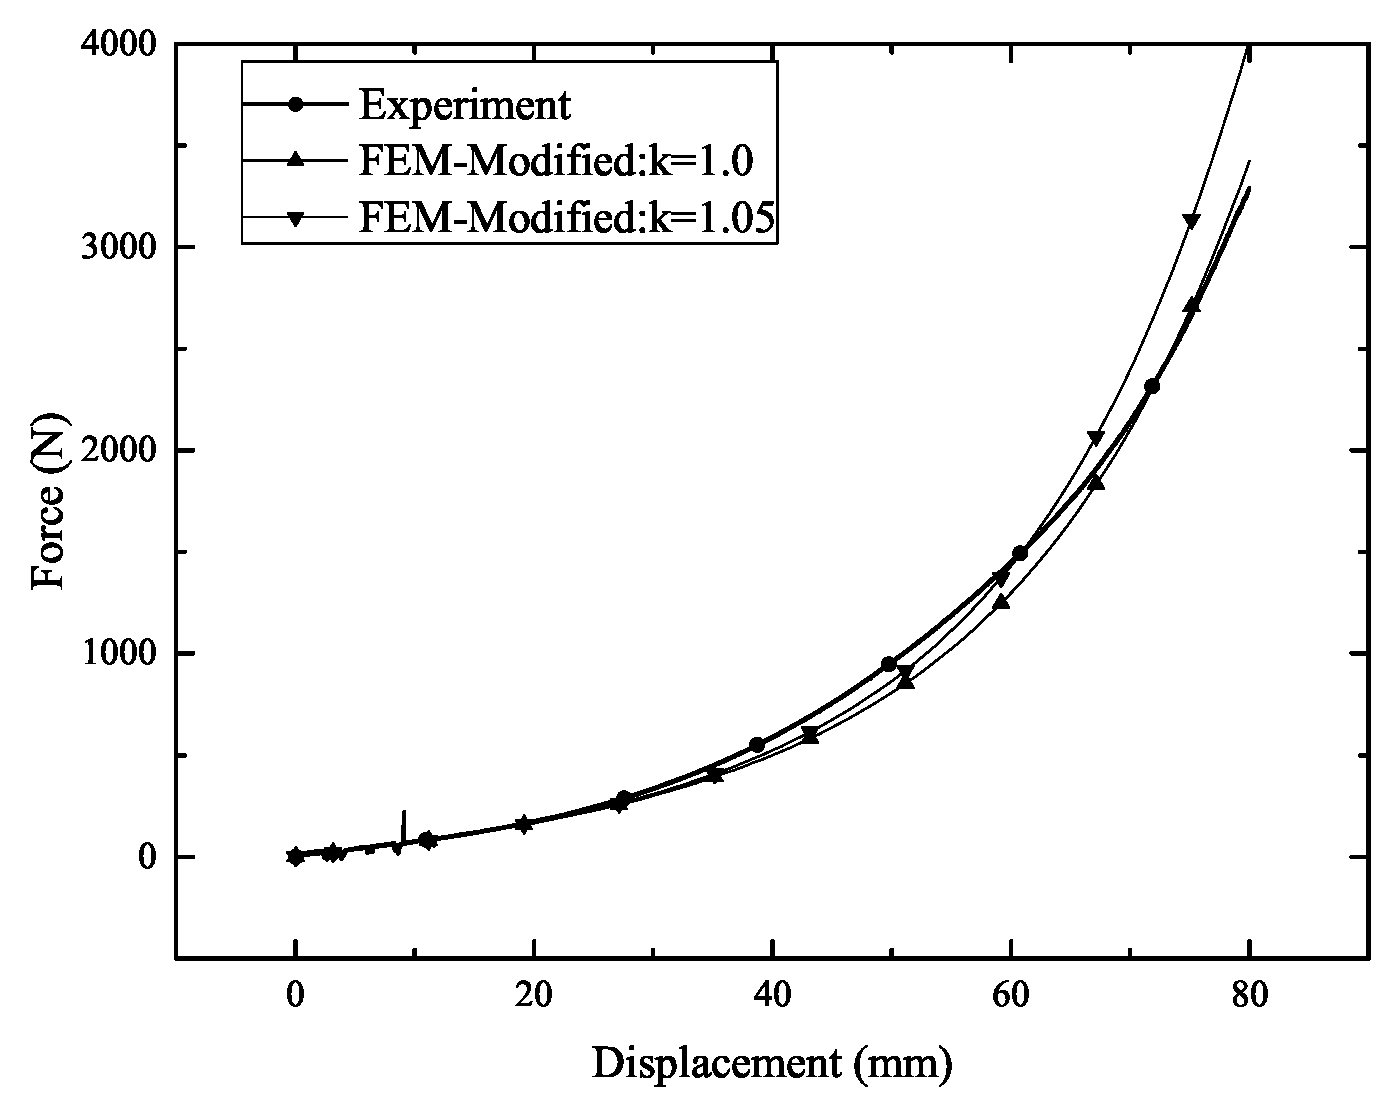
\includegraphics[width=0.7\linewidth]{figure/chap5/sp1/k-mod}
	}
\subfigure[实验试件-2]{
	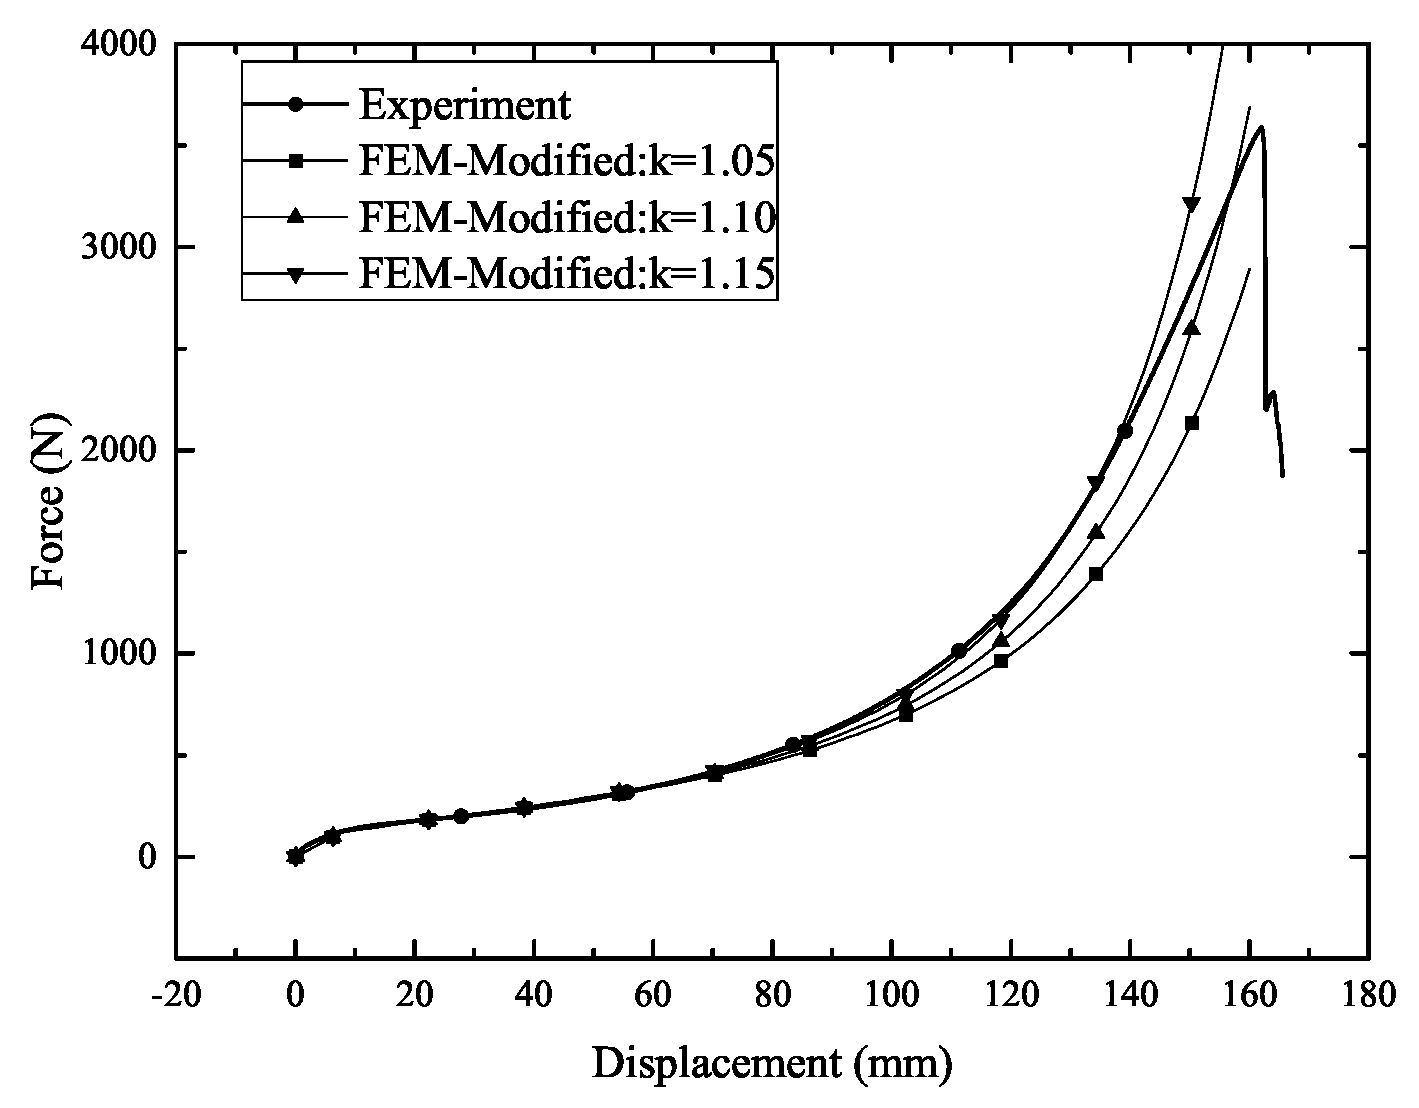
\includegraphics[width=0.7\linewidth]{figure/chap5/sp2/k-MOD}
	}
\fcaption{不同编织角加速系数的影响}{}
\label{fig:k-MOD}
\end{figure*}

综合调整其他参数,实验试件-1取$ V_W=1.0$,$ k=1 $;实验试件-2取$ V_W=0.7 $,$ k=1.12 $,仿真结果如\ref{fig:final}所示。

相比 未修正的\ha 基本理论,综合各项影响因素的修正理论基本上可以完全拟合拉伸实验所得到的力位移曲线。所得到的本构理论,从刚度上来说是可信的。从有限元仿真的角度来说,可以较简便地应用于内压爆破实验的仿真。 

\begin{figure*}[!htbp]
\centering
\subfigure[实验试件-1]{
	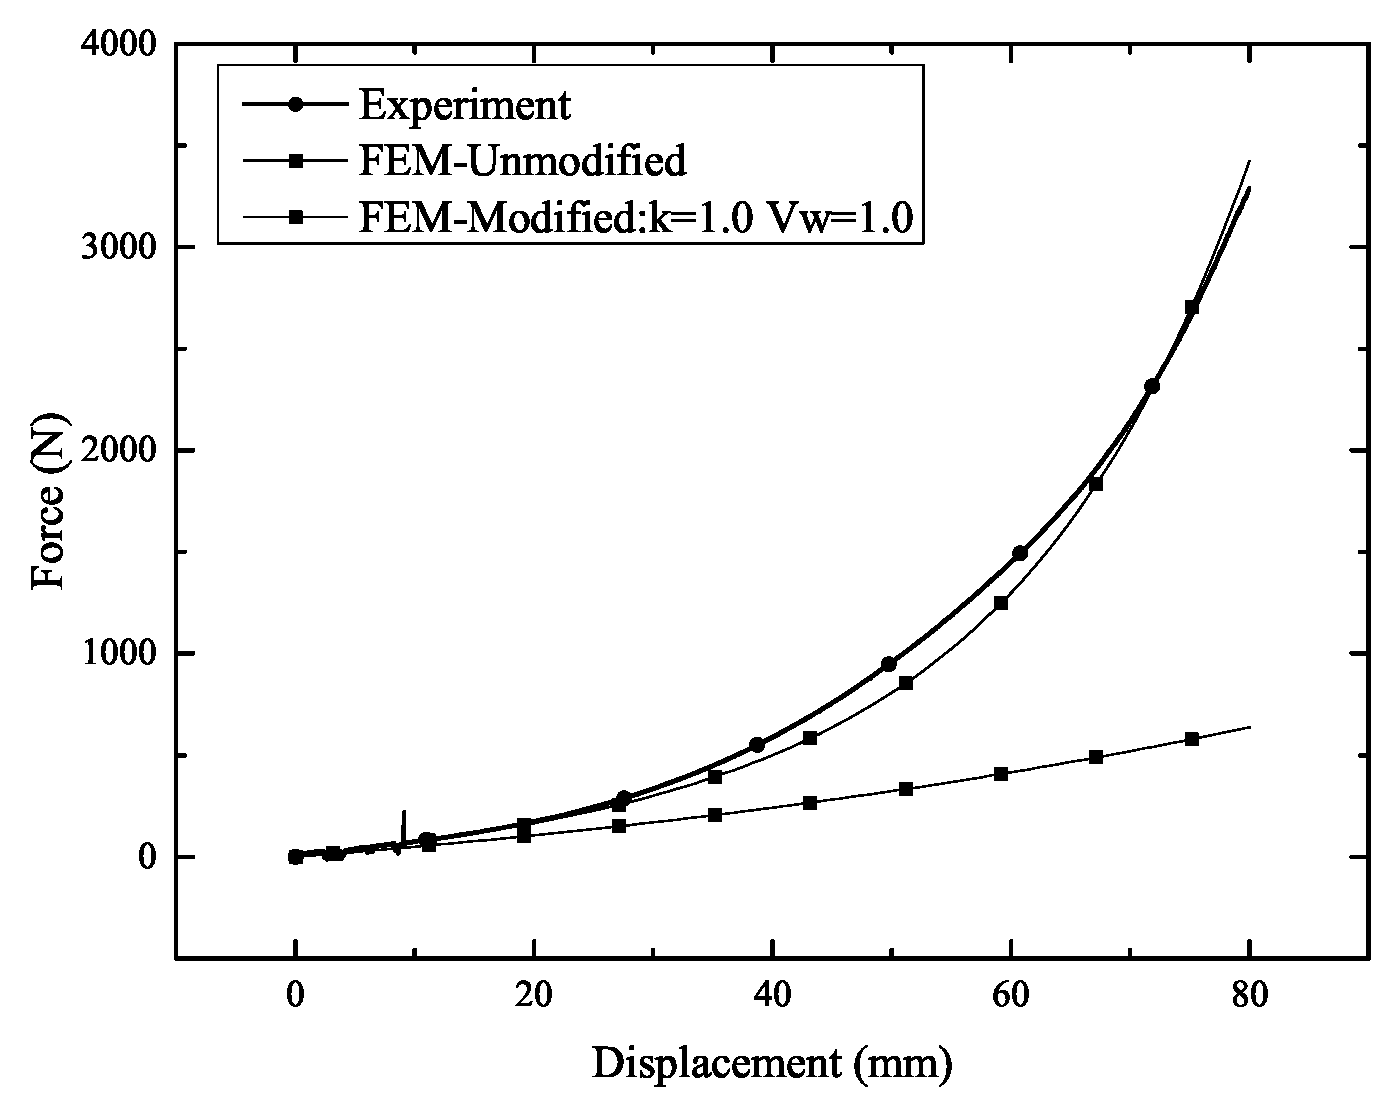
\includegraphics[width=0.7\linewidth]{figure/chap5/sp1/final}
;}
\subfigure[实验试件-2]{
	\includegraphics[width=0.7\linewidth]{figure/chap5/sp2/final}
}
\fcaption{综合修正有限元仿真结果}{}
\label{fig:final}
\end{figure*}





%%==================================================
%% chapter03.tex for TJU Master Thesis
%% Encoding: UTF-8
%%==================================================

\chapter{编织层准静态强度及内压爆破实验仿真}


\section{引言}

前面一章针对编层的非线性力学行为,进行了理论体系的修正和拓展,取得了较好的效果,本章则是对该理论模型在内压荷载的应用。
首先,本章要明确该理论体系如何确定特征单元的应力应变状态与编织层纤维应力应变状态,这实际上是与前一章中“平均化”相反的过程。
其次,本章要明确如何将理论结果应用到内压爆破试验中去。因为内压爆破试验是一个动态加载的过程,而前一章中得到的理论体系实际上是在准静态的条件下得到的。

\section{准静态强度判定}

编织层特征单元的应力应变状态可以通过特征单元的几何关系推导出编织层纤维的伸长量。而纤维本身的额定破坏应力的大小决定了纤维的最大伸长率。可以以此作为判断编织层是否发生破坏的准则:

\begin{equation}
{\sigma _f} = {\varepsilon _f} \cdot E \le \left[ {{\sigma _u}} \right]
\end{equation}

根据特征单元的几何关系,如图\ref{fig:unit-cell-chap6}所示,编织层纤维的纤维向应变$  \sigma _f$为:


\begin{figure*}[!htb]
	\centering
	\includegraphics[height=0.25\textheight]{figure/chap5/unit-cell-3}
	\fcaption{特征单元的纤维方向伸长}{elongation of the representative unit cell in fiber direction}
	\label{fig:unit-cell-chap6}
\end{figure*}


\begin{equation}
\label{eq:fiber-elongation}
{\varepsilon _f} = \sqrt {\frac{{{{\left( {{\varepsilon _{22}} + 1} \right)}^2} + \tan {\alpha ^2}{{\left( {1 - {\varepsilon _{33}}} \right)}^2}}}{{1 + \tan {\alpha ^2}}}}  - 1
\end{equation}



\subsection{拉伸实验仿真结果对比}

对比数值模拟的拉伸实验仿真结果,接头颈缩处为纤维伸长量最大处(图\ref{fig:strength}云图中红色区域)与实验结果吻合,应力大小为2000MPa,与实验金属纤维的额定模量一致。可以认为该理论对于准静态的加载状态有效。

\begin{figure*}[!htb]
\centering
\emph{}\includegraphics[height=0.25\textheight]{figure/chap6/strength}
\fcaption{修正模型仿真拉伸实验纤维应力分布云图}{stress in fiber direction with modified model}
\label{fig:strength}
\end{figure*}

\ha 基本理论事实上并没有考虑编织层强度的算法,但根据其特征单元同样可以求出纤维也可以推得的纤维向应变 ,

\[{\varepsilon _f} = \sqrt {\frac{{{{\left( {{\varepsilon _{22}} + 1} \right)}^2} + \tan {\alpha ^2}}}{{1 + \tan {\alpha ^2}}}}  - 1\]

\begin{equation}
= \cos \left( {\alpha  - d\alpha } \right)\cos \alpha  \cdot {\varepsilon _{22}} - \frac{{{{\left( {d\alpha } \right)}^2}}}{2}
\end{equation}

上式基于未修正的特征单元几何模型,在特征单元的层面上,并没有考虑管径变化对纤维应变的影响。而从钢绞线理论出发,研究发现是很难回归到纤维方向的应变上的。
利用该式得到的纤维向应力云图\ref{fig:hose-strength002}, 
并不能得到正确的应力分布,发生断裂的接头处纤维的反而是应力最小处,显然不能将该理论应用于编织层的设计。
\begin{figure*}[!htp]
	\centering
	\includegraphics[height=0.26\textheight]{figure/chap6/hose-strength002}
	\fcaption{未修正拉伸试验纤维应力分布}{ stress in fiber direction with Hachemi's model}
	\label{fig:hose-strength002}
\end{figure*}

 






\section{内压爆破强度判定}

由于内压爆破实验的加载过程升压速率非常快,不能视为准静态过程。但是该过程的振动、激励不是研究的重要对象,仅仅需要研究金属纤维最终是否会断裂。因此这里通过材料力学中的突加荷载的方法,利用荷载系数修正准静态加载的结果,将准静态的应力应变状态乘以突加荷载系数2,就可以得到爆破内压实验荷载下编织层纤维的应力应变状态。当然,该系数是偏安全的。

\begin{equation}
2\sigma _{static}= \sigma _{burst}
\end{equation}

因此,利用本文修正后的理论,可以采用准静态的方法对软管组件内压爆破实验进行仿真分析。在准静态的分析中,只要满足:
\begin{equation}
{\sigma _f^{static}}  \le \frac{1}{2} \left[ {{\sigma _u}} \right]
\end{equation}

就可以认为纤维尚未发生断裂,该压力下软管组件安全。$ {\sigma _f^{static}} $为准静态分析中纤维上的应力。


\subsection{内压爆破仿真}

进行内压实验的有限元仿真,同样采用\uma 导入本文的理论模型。首先根据确定的软管组件的规格进行完整的几何建模,然后逐步开始施加内压荷载。当发现纤维方向的应变$ \varepsilon_f $达到极限应力对应的应变的二分之一时,停止增加内压荷载,此时内压荷载的大小就是该规格软管组件的爆破压力值。图\ref{fig:chap6-hose-burst}为不同规格软管组件受内压荷载是的状态。



本文首先对Φ5(10.5MPa)软管组件进行了内压爆破的仿真\footnote{内压爆破实验数据由上海市塑料研究所提供},验证修正非线性段软管组件的本构修正对内压爆破荷载仿真效果的影响。因其经过拉伸实验验证,可以对比拉伸力位移曲线的拟合程度对爆破压力仿真值的影响。仿真结果的纤维向应力值由式\ref{eq:fiber-elongation}求得。


\begin{table}[!htbp]
	\centering
	\tcaption{ Φ5(10.5MPa)软管组件内压模型修正效果}{Φ5(10.5MPa)hose modified FEM results contrast}
	\label{tab:strength-of-hose-results}
	\begin{tabular}{@{\extracolsep{\fill}}>{\hspace{0.5cm}}clcccc}
		\toprule
		&平面内纤维&斜穿纤维&加速系数&爆破压力&相对误差\\\midrule
		修正-1&0.5&0.5&1.15&96.7MPa&0.31\%\\
		修正-2&0.5&0.5&1&94.9MPa&-1.56\%\\
		未修正&1&0&1&84.5MPa&-12.34\%\\
		\bottomrule
	\end{tabular} 
\end{table}  


表\ref{tab:strength-of-hose-results}给出了不同修正参数求得的爆压力值,而各组修正参数对应的拉伸力位移曲线如图\ref{fig:strength-elongation}所示。


\begin{figure*}[!htp]
	\centering
	\subfigure[不同修正参数软管拉伸力位移曲线]{
		\includegraphics[width=0.5\linewidth]{figure/chap6/Graph152}	
		\label{fig:strength-elongation}
	}
	\hspace{0.5cm}
	\subfigure[软管受内压荷载变形]{
		\includegraphics[width=0.25\linewidth]{figure/chap6/stress}
	}
	\fcaption{内压爆破试验仿真效果}{burst pressure simulation results}
	\label{fig:stress}
\end{figure*}


根据表\ref{tab:strength-of-hose-results}给出的仿真结果,可以发现,\ha 理论计算的爆破压力值,对比修正模型,误差较大。
分析认为:\ha 理论在只在线性段拟合的比较好,而内压爆破荷载下软管的变形,大部分发生在线性段,小部分发生在非线性段,并不像拉伸实验那么明显,因而\ha 未修正的仿真结果大致正确 。








\begin{table}[!htb]
	\centering
	\tcaption{ 不同规格软管组件实验及有限元爆破压力}{exprimental and FEM caculated burst pressure of hoses}
	\label{tab:strength-of-hose}
	\begin{tabular}{@{\extracolsep{\fill}}>{\hspace{0.5cm}}clcccc}
		\toprule
		序号 &    规格     & \tabincell{c}{编织形式\\/mm×根 }& \tabincell{c}{实际\\爆破值/MPa }& \tabincell{c}{计算\\爆破值/MPa}& \tabincell{c}{偏差\\百分比}  \\ \midrule
		1  & Φ5(10.5MPa)  & Φ0.2×6  &   96.4    & 96.7          & 0.31\% \\
		2  & Φ8(10.5MPa)  & Φ0.3×5  &   83.5    & 83          & -0.60\% \\
		3  & Φ12(10.5MPa) & Φ0.3×6  &   63.5    & 66          & 3.94\%  \\
		4  & Φ16(5.0MPa)  & Φ0.3×6  &   47.1    & 51          & 8.28\% \\ \bottomrule
	\end{tabular} 
	\end{table}  

修正后的理论模型可以考虑非线性段的影响,仿真求得的爆破压力值更接近大量实验的统计值。对不同规格的软管组件采用$ V_w=0.5,V_s=0.5,k=1.0 $的修正参数对编制层的刚度进行修正。仿真爆破压力值如表\ref{tab:strength-of-hose}所示。

\begin{figure*}[!htp]
	\centering
	
	\subfigure[]{
		\includegraphics[height=0.33\textheight]{figure/chap6/1}
		\label{fig:chap6-1}
	}
	\subfigure[]{
		\includegraphics[height=0.33\textheight]{figure/chap6/2}
		\label{fig:chap6-2}
	}
	\fcaption{不同规格软管组件内压爆破实验仿真}{deformation of hose under burst pressure with modified model}
	\label{fig:chap6-hose-burst}
\end{figure*}


几组软管的爆破压力值计算误差都在$ 10\% $以内,可以认为该算法稳定有效。


\section{小 ~ 结}

本章主要利用前文修正的纤维编织层本构模型,对内压爆破实验进行了仿真,对比了爆破实验的数据,验证了通过拉伸实验修正的理论可以应用与不同工况的仿真。

在进行内压爆破的仿真之前,本章推导了修正理论模型在纤维方向上的应变的计算方法,对拉伸实验进行了强度的验证。

然后,本章利用材料力学突加荷载理论,利用准静态的仿真,等效模拟内压爆破荷载的工况,并提出了强度换算的方法。

%%==================================================
%% conclusion.tex for SJTU Master Thesis
%% based on CASthesis
%% modified by wei.jianwen@gmail.com
%% version: 0.3a
%% Encoding: UTF-8
%% last update: Dec 5th, 2010
%%==================================================

\chapter*{全文总结\markboth{全文总结}{}}
\addcontentsline{toc}{chapter}{全文总结}

这里是全文总结内容。





\appendix	% 使用英文字母对附录编号,重新定义附录中的公式、图图表编号样式
\renewcommand\theequation{\Alph{chapter}--\arabic{equation}}	
\renewcommand\thefigure{\Alph{chapter}--\arabic{figure}}
\renewcommand\thetable{\Alph{chapter}--\arabic{table}}


%%==================================================
%% Encoding: UTF-8
%%==================================================

\chapter{模板更新记录}
\label{chap:updatelog}



\backmatter	% 文后无编号部分 

%% 参考资料
\bibliography{bib/preference}



%% 致谢、发表论文、参与项目、简历
%%==================================================
%% thanks.tex for SJTU Master Thesis
%% based on CASthesis
%% modified by wei.jianwen@gmail.com
%% version: 0.3a
%% Encoding: UTF-8
%% last update: Dec 5th, 2010
%%==================================================

\begin{thanks}

  感谢所有测试和使用交大学位论文 \LaTeX 模板的同学!

  感谢那位最先制作出博士学位论文 \LaTeX 模板的交大物理系同学!

  感谢~William Wang~同学对模板移植做出的巨大贡献!

\end{thanks}
 	%% 致谢
%%==================================================
%% pub.tex for SJTU Master Thesis
%% based on CASthesis
%% modified by wei.jianwen@gmail.com
%% version: 0.3a
%% Encoding: UTF-8
%% last update: Dec 5th, 2010
%%==================================================

\begin{publications}{99}



\item {\bf 胡牧原}, 郑百林, 贺鹏飞等. 基于非线性本构关系的软管编织增强层等效刚度修正方法研究[J]  力学季刊, 2015,V36(1): 70-   (国内核心)
	
\item {\bf 胡牧原}, 郑百林, 贺鹏飞等. 基于非线性本构关系的软管编织增强层等效刚度修正方法研究[J]  力学季刊, 2015,V36(1): 70-   (国内核心)


\item Hu T Y, Zheng B L, {\bf Hu M Y}, et al. Molecular dynamics simulation of incipient plasticity of nickel substrates of different surface orientations during nanoindentation[J]. Materials Science and Technology, 2015, 31(3): 325-331.(SCI)

\item 冯敏, \textbf{胡牧原}, 郑百林, 等. 基于 Abaqus 二次开发用户白定义场的功能梯度材料人体骨骼建模[J]. 计算机辅助工程, 2013, 22(5): 112-116.


\item 胡腾越, 郑百林, \textbf{胡牧原}, 等. 纳米压痕中位错运动的原子模拟[J]. 力学季刊, 2014, 2: 006.	
    
\end{publications}

\textbf{个人简历\LARGE}


胡牧原,男1989年4月生

2012年7月,毕业于长安大学理学院,工程力学专业,获工学学士学位。

2012年9月,开始攻读同济大学航空航天与力学学院硕士学位。	%% 发表论文
%%==================================================
%% projects.tex for SJTU Master Thesis
%% based on CASthesis
%% modified by wei.jianwen@gmail.com
%% version: 0.3a
%% Encoding: UTF-8
%% last update: Dec 5th, 2010
%%==================================================

\begin{projects}{99}

    \item 973项目“XXX”
    \item 自然基金项目“XXX”
    \item 国防项目“XXX”
    
\end{projects}
  %% 参与的项目
% \include{backmatter/resume}

\end{document}
